\documentclass[12pt,a4paper]{report}
\usepackage{Bath-CS-Dissertation}
\graphicspath{{./}}
\title{\bf Flower Species Recognition on a Smartphone}
\author{Saahil Shihaz}
\date{Bachelor of Science in Computer Science\\
    The University of Bath\\
    2021-2022}
\begin{document}
\hypersetup{pageanchor=false}
\setcounter{page}{0}
\pagenumbering{roman}
\maketitle
\newpage
\consultation{0}
\newpage
\declaration{Flower Species Recognition on a Smartphone}
{Saahil Shihaz}
\newpage
\hypersetup{pageanchor=true}
\begin{abstract}

    The evolution of smartphones over time has made them more capable of complex tasks. One such task is image 
    classification. This is where a computer attempts to identify an object or many objects within an image and give 
    them a label. Classifiers can be built using machine learning (ML) by training models with example data so that they 
    can attempt to recognise new data it hasn't seen before. 
    
    \par
    
    Deep learning (DL) is a part of ML and has undergone large advancements in
    recent years. Recently, libraries like TensorFlow allow developers to implement DL models within 
    smartphones. The state of the art will be highlighted within the project to provide a deep understanding of the 
    context. Then an investigation is conducted to compare classification approaches for recognising flower species. The
    Inception V3 model is demonstrated to be very effective in identifying flowers within the Oxford Flowers 102 
    dataset, with an accuracy of 95.7\%. An Android app will then be designed and developed using the latest available 
    APIs to demonstrate the capabilities of the DL model within a smartphone by analysing how well the classifier 
    performs. 

\end{abstract}
\clearpage
\tableofcontents
\clearpage
\listoffigures
\listoftables
\clearpage
\chapter*{Acknowledgements}

I would like to thank my supervisor, Hongping Cai, for their valuable feedback and insight which helped improve the 
quality of the project. They provided me with great resources to help my understanding of the research topic and
supported me through the entire year.

\par

I would also like to thank my fellow coursemates for providing me with their support throughout the year. They
really helped motivate me.

\par

Finally, I would like to thank my friends and family as they would happily listen to me discuss my project and allow me
to test my app on some of their flowers.

\clearpage
\pagenumbering{arabic}
\chapter{Introduction}

This chapter will outline the overall plan for this dissertation, starting with an in-depth look at the problem and a 
brief look at the domain.

\section{Problem Description}

The technological era that we live in has introduced many groundbreaking achievements that constantly push the barrier 
of what is possible as well as introduce many new challenges that require complex solutions. One such challenge is big 
data processing, specifically, recognising patterns in data and drawing conclusions. Unfortunately, machines don't have 
the ability to understand data the way that humans do and humans don't have the processing capabilities of modern 
machines. Due to obvious ethical and biological barriers, humans cannot fill the role of computers that compute 
data on a large scale therefore, the alternative must be explored; making computers as smart as humans. This is where 
Machine Learning (ML) steps in. What this project will focus on in particular,
is granting the advanced capabilities of ML to smartphones.

\par

This project aims to investigate the application of ML techniques to recognize images of flower species 
on smartphones. This will be done by implementing classical ML algorithms that are effective in image 
classification as well as Deep Learning (DL) algorithms which are stated to be more effective in carrying out the same 
task. It will be interesting to compare both types of implementations in terms of accuracy and speed.

\par

Smartphones have the advantage of portability and flexibility compared to PCs at the expense of pure processing 
power, storage and battery life. Advancements in ML can boost the abilities of smartphones by allowing 
them to make informed decisions to aid the user. Traditional algorithms can't answer questions
like “What is this flower?”
without being cumbersome and inaccurate, that's why ML is required.
Smartphones and tablets are packed with more powerful technology than they've ever had like advanced
cameras, sensors, displays and processors. Each of these are resources that an ML model can take advantage of.

\par

Traditionally, smartphones as well as similar devices do some light pre-processing of data, then they 
send it to the cloud which can handle actions that require intensive processing, this introduces some level of latency 
because of the communication between the device and the cloud \citep[p. 3]{olascoaga2021hardware}. 
Latency is important to consider in some use cases such as autonomous vehicles \citep[pp. 3-4]{olascoaga2021hardware} 
where it may be important for a vehicle to make quick decisions about potential obstacles.

\par

With some raw information, a classical ML process can identify features, these could be used by a 
classifier that can make predictions given a set of data it hasn't seen before \citep{lecun2015deep}. Features are 
sourced from the representation of an object, in turn, the representation is defined by the 
data input. An example of a feature would be the presence or absence of thorns on the stem of a flower 
\citep[p. 22]{goodfellow2016deep}. Traditional ML practices incorporated 
feature engineering that required designing custom algorithms for a particular task which can be time-consuming 
\citep{liu2020representation}. There is also difficulty in understanding what features should be extracted, 
for example, it may be hard to represent flower petal shapes properly from raw pixel values if there are shadows being 
cast on them \citep[p. 23]{goodfellow2016deep}. Representation learning is a method that 
can fix such issues by providing mappings, not from just the representation of data to the output, but from 
representation to representation \citep[p. 24]{goodfellow2016deep}. There are, however, 
still hurdles to overcome, these are described as “factors of variation” where external factors might affect the source 
data, such as the age of a flower, which could affect the petal shape and the season which may affect a flower's 
appearance. Factors like this make it difficult to get representations in the first place 
\citep[p. 24]{goodfellow2016deep}.

\par

DL is a part of ML that aims to overcome the limitations of classical ML techniques 
by expanding upon representation learning. DL can be split into two unique parts:

\begin{itemize}
    \item \textbf{Distributed Representation:} These are used to represent objects in a more compact and dense manner.
Instead of having representations for each type of object, for example, a collection of words in a sentence, one could 
store the frequency of each word like the bag-of-words problem \citep{liu2020representation}. This is a sparse
representation and introduces problems with space and time complexity. Therefore, distributed representations aim to 
tackle the sparsity problem as they are harder to model \citep{Brownlee2017}.
    \item \textbf{Deep Architecture:} The idea of layering to represent neurons in a human brain. It can be imagined 
    as a map of 
nodes that takes an input and then processes it through the different layers where at each step, a set of units calculate a 
weighted sum of their inputs from the previous layer to then pass the result to the next layer until it gets to output units
that generate a result. This is an example of a feedforward neural network \citep{lecun2015deep}.
\end{itemize}

\par

Input into a DL algorithm starts at the visible layer, which contains a set of input pixels that can be
directly observed. This data is passed into a network of hidden layers, each of these layers represents an abstract 
feature that can't normally be observed by looking at the input data such as locations of edges and contours 
\citep[p. 26]{goodfellow2016deep}.

\par

By making use of TensorFlow, developers can produce classification models using languages like Python, C++ or Java, then 
convert said models into small packages that an Android/IOS application can use to generate predictions based on an 
input. TensorFlow is developed by Google and provides a suite of tools to design, test and 
deploy ML solutions. The Lite version of TensorFlow will be used in this project and is designed specifically for mobile and Internet of 
Things (IoT) devices 
that may not have the support of powerful hardware. Using TensorFlow, it is possible to develop DL models like 
Convolutional Neural Networks (CNN) \citep{googleTF2}. 
There are examples that can be built specifically for flower classification within the documentation which can serve
as a starting point for the project.

\section{Main Objectives}
The main objectives serve as a plan to first, understand the domain, 
identify the key resources, experiment with approaches and then finally create a product that encapsulates 
everything that was learnt in this project. This is what I hope to achieve for this project:
\begin{itemize}
    \item Identify and review literature that will aid in understanding the problem domain.
    \item Analyse existing smartphone-based image recognition software.
    \item Investigate the advantages and disadvantages of both classical ML and DL implementations and compare the two 
using analysis tools, this will be done on PC hardware.
    \item Design and implement an Android application that can recognize images using DL.
    \item Discuss the feasibility of DL on smartphones.
    \item Explore future improvements for the Android app.
\end{itemize}

\section{Structure}

This dissertation will consist of the following chapters:
\subsubsection*{Introduction}
A look at the subject domain to outline what this dissertation will be about. The problem description and objectives are
presented here.

\subsubsection*{Literature and Technology Review}
A presentation of the background research relevant to this dissertation. Here the subjects of ML and DL will be
expanded upon. Additionally, the topic of flower classification will be elaborated on by looking at existing solutions.

\subsubsection*{Investigation}
An investigation into the classification approaches for classical ML and DL. Here, there will be two implementations that
will be presented and analysed.

\subsubsection*{Flower Classification App}
The development and implementation of a flower classification app based on the findings in the literature and 
technology review as well as the investigation.

\subsubsection*{Conclusion}
A reflection of the dissertation that includes contributions and a critical appraisal.

\clearpage
\chapter{Literature and Technology Review}

Ground-breaking achievements in technology have given developers the tools and capabilities to
tackle the key problem of image recognition. What this project aims to demonstrate is the application of DL 
within a smartphone application to recognise flowers. It will be interesting to see how it performs on smartphone 
hardware which is generally less powerful than desktop PCs and laptops. Additionally, it will be beneficial to explore 
what sort 
of optimisations need to take place in order to get a feasible smartphone-based solution. The limited computing resources 
that are available to developers when creating their solutions is what makes DL on smartphones challenging. 
Smartphones typically 
contain smaller processors, storage and batteries. These restrictions are in place to 
make them more efficient and to ensure that they last longer when not connected to a power source. In addition
to this, the subject of ML (and subsequently DL) is complex and many find the concepts challenging to understand. 
What this literature review aims to do is identify key sources of information to help break down the underlying 
subject and discuss the quality of the research available.

\section{Mobile Machine Learning}

The potential of smartphones has still not been fully realised. With advancements in ML, developers can take the 
capabilities of smartphones to the next level by leveraging the advanced hardware within them to carry out complex 
tasks. This section will identify the key milestones within smartphone technology and how it leads to integrating 
ML to make full use of the hardware.

\begin{figure}[h]\
    \centering
    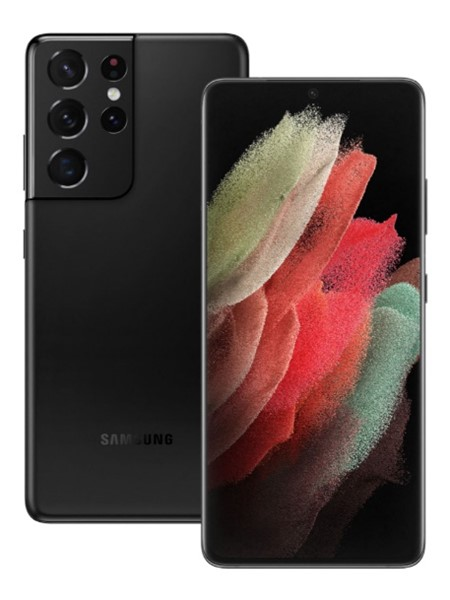
\includegraphics[width=0.3\textwidth]{s21ultra.jpg}
    \caption{Samsung Galaxy S21 Ultra 5G: Boasting an impressive array of camera sensors on the back \citep{three2021}.}
\end{figure}

\break

\subsection{Evolution}

Firstly, it is worth looking at the last 10 years of technological advancements within the smartphone space. 
With this information, some insight may be gained into how much their capabilities have evolved. To do this, some
aspects of specification data have been collected from the Samsung Galaxy flagship line of smartphones. Samsung 
currently holds the top spot in global market share at 20.8\% as of Q3 2021, this position is typically held by Apple or
Samsung and can vary from a quarter to quarter basis \citep{odea2021}.

\par

By looking at the table in Appendix \ref{sec:smartphones}, it is clear there has been an increase in 
smartphone capabilities within 
multiple categories like the processor speed, core count, 
storage, memory and camera. There are, of course, many more different areas that are not listed like sensors, 
screen size and battery life which have also seen massive improvements over the last 10 years. It is safe to
assume that improvements will continue to be seen in the near future. 
What must also be considered is price and accessibility; flagship smartphones represent the top of the line offerings from
each manufacturer and are of course priced as such. Low to mid-end smartphones are still more capable 
than their predecessors albeit their spec sheet may not be as impressive as high-end versions in the same generation. 
Developers must ensure some level of scalability within their ML processes to ensure they can run on a wide range of
devices and not just the most powerful.

\par

\citet{kulendran2014} highlights how improvements in smartphones have created a boom in the number of 
smartphone-based applications designed to aid surgeons and patients in multiple facets of the medical industry like 
plastic, orthopaedic and general surgery. They conduct an expansive review of different solutions and analyse how the 
evolution of smartphones got them to the point that makes them extremely useful as a tool to aid people. Ultimately, what 
this project aims to do is provide a robust software solution to recognise flower species on a smartphone, however it
cannot be ignored that smartphones have come a long way in the hardware and software space to allow the
conception of such a system.

\subsection{Where does this lead us to, today?}

ML and AI have become such an important part of smartphones that manufacturers now have dedicated processors for these
types of tasks. Google includes a Tensor Processing Unit (TPU) in their Pixel line of phones \citep{triggs2021}. Samsung, 
Qualcomm and Apple use their own solutions for ML by having their own bespoke processors. These 
processors are used to compute specific actions that require the decision making and accuracy capabilities of ML.
Google Tensor in particular powers tasks such as speech recognition in a way that makes it more accurate and less taxing,
therefore 
saving battery life. Tensor also applies to processing photographs and provides additional features to videos 
\citep{gupta2021}. With such a focus on smartphones, to the point that they get dedicated hardware for ML,
a huge increase in applications that integrate ML in some way should be seen, as well as the entire process of designing
and implementing such solutions being carried out more rapidly, as developers learn to leverage the hardware.

\section{Computer Vision}

Since this research heavily involves processing visual data, the area of computer vision plays a big part in this 
research. In order to identify flower species, the techniques used to analyse the incoming image data to make 
predictions using ML must be discussed.

\subsection{History}

\citet{SzeliskiRichard2011CV:A} outlines significant occurrences in each decade starting from the 70s, 
thought to be the beginning of computer vision, all the way through to the 2000s. In the early 70s, researchers sought 
to emulate human intelligence in a machine by first solving "the visual problem". It was hypothesised that if a computer 
could first recognize objects in the real world that it could then move on to the next step of using reasoning and 
problem-solving at a high level. The first processes conducted to understand the 3D world were to extract edges to 
recognize 3D objects from 2D lines in an image.

\par

The 80s were described to have a lot more focus on mathematical techniques for analysing scenes. Various algorithms 
and models were conceived as well as improvements in the contour and edge detection space. Researchers found that a 
lot of these algorithms could be thought of as “optimization problems” when they were described using the same 
mathematical framework.

\par

Some more improvements can be observed in the field during the 90s including the production of 3D surfaces, tracking 
and image 
segmentation. However, what is probably more relevant to this project is statistical learning techniques that also 
started to appear during this decade. In 1991, a paper by \citet{turk1991face} describes
the concept of “eigenfaces”. These are the product of converting images of faces into feature images. These feature 
images are essentially the training set. Recognition occurs “by projecting a new image into the subspace spanned by 
the eigenfaces”. The new face is then classified by comparing its position relative to the known set of faces. 
Emphasis was placed on limiting the scope of the allowed images, as such the system was trained and ready to 
accept profile straight-on images of the subject. In addition, they aimed to have the system compute a result
in a reasonable time. This is one of the goals of this project, as it would be counter-intuitive to have an ML algorithm 
that takes a significant amount of time to compute an answer.
The research hoped to improve on its 
predecessors that used at the time, traditional methods of recognising features such as eyes, noses and mouths and 
their relative position to each other. The work done with eigenfaces shows great similarities with the ML
techniques seen today, by essentially creating feature vectors and comparing the distance of known 
vectors in the same space.

\par

\citet{SzeliskiRichard2011CV:A} continues with their insight into the 2000s, where they outline the various 
improvements like more efficient algorithms and what finally dominates the latter half of the 2000s; applying ML 
techniques to computer vision to aid visual recognition research.

\section{Machine Learning}

This project will aim to produce ML algorithms to compare efficiency and accuracy to the more evolved DL. 
Firstly, the building blocks of ML must be looked at to get a deeper understanding. 
\citet{CamastraFrancescoMLfA} summarise this area and broke down ML development around three primary research 
points:

\begin{itemize}
    \item \textbf{Task-Oriented Studies}: Improving the performance of learning systems in a predetermined set of tasks.
    \item \textbf{Cognitive Simulation}: Emulating the human brain and designing processes around the human thought process.
    \item \textbf{Theoretical Analysis}: “The theoretical investigation of possible learning methods and algorithms 
    independently of application domain”.
\end{itemize}

They also produce a taxonomy to represent the balance of two entities they describe: the “teacher” and the “learner”. 
The teacher is the programmer, the one that designs the learning process and the learner is the computer system. 
The idea of inference is also introduced where a system can derive knowledge from previous observations. The taxonomy 
breaks down the amount of work that both the “learner” and the “teacher” need to do into four categories: Rote Learning,
Learning from instruction, Learning by analogy and Learning from examples.

\par

What this project will make use of is learning from examples where the “learner” infers the most out of the other 
categories in the taxonomy. The idea of the “learning problem” is introduced where the system needs to find a “general 
rule that explains the data given only a sample of limited size”. Learning techniques are broken down into four more 
categories: Supervised learning, Reinforcement learning, Unsupervised learning and Semi-supervised learning.

\par

\citet{zhu2005semi} highlights semi-supervised learning in their survey as the combination of supervised and
unsupervised 
learning where both labelled and unlabelled data is used for the training of the classifier. They point to the survey done by
\citet{seeger2000learning} in particular that provides more insight into the concept of semi-supervised 
learning. Their rationale for the concept was to produce the ability for a system to make predictions based on 
the knowledge it doesn't have. A supervised system has all labelled data to aid its training therefore its basis for making
predictions is described as a “security belt” by Seeger. The model will basically make predictions within its limited 
scope, this is called “overfitting” \citep{tom1995}. Unsupervised learning heavily relies on prior assumptions for 
its final result, this is because it doesn't have a knowledge base to rely on. By using a combination of both 
implementations, one can “balance the impact of prior assumptions”. Seeger also highlights the fact that labelling the 
data is a taxing process. Fortunately for this project, datasets already exist with labelled images for 
flower species.

\subsection{Feature Extraction}

\citet{dishaa2021} provides an introductory guide to feature extraction. They describe feature extraction 
as one of the two ways to reduce dimensionality with the other being feature selection. Extraction produces new 
features which are described as a “linear combination of the existing features”. The process aims to use fewer features to 
encapsulate the same image information.

\par

\citet{tian2013} conducts a review of image feature extraction techniques that are worth considering. They 
start by discussing extracting colour features such as histograms and colour “moments” from specific colour spaces 
such as RGB and HSV. This feature will be important as flowers come in many different colours, but it 
cannot solely be relied on as different species can share similar colours. The paper also compares different types of colour features such as outlining histograms being simple to 
compute but also having sensitivity to noise. The texture of an image can also be extracted, this is where 
groups of pixels begin to be analysed together. Texture in the 
context of images is a way to describe the perceived smoothness, roughness or bumpiness of an image through spatial 
variations in pixel intensity levels \citep{mathworks}. Lastly, the paper goes into depth about shape features and 
points to different sources that go into the subject. To summarise, shape features are 
split into two broad categories: contour and region based. This is where the features are calculated from shape 
boundaries and image regions respectively. A simple example of a shape feature is the circularity ratio where one measures 
how close a shape is to a circle by calculating the ratio of the area of a shape to the area of a circle with the same 
perimeter \citep{mingqiang2008survey}. Shape analysing will be very important in this project because flower shapes can
differ greatly and can therefore serve as a way to easily differentiate between species.

\subsection{Classification}

\citet{brownlee2020} provides an easy-to-understand breakdown of classification within ML. They describe it 
as the process of assigning “a class label to an example from the problem domain”. In the context of this project, that 
means classifying a 
flower as species A as opposed to B, C or D. They also go into detail about the different classification methods such 
as:
\begin{itemize}
    \item \textbf{Binary classification}, e.g. it's flower A or flower B.
    \item \textbf{Multi-class classification}; where there are more than two classes.
    \item \textbf{Multi-label classification}; this is where there are multiple predictions for classes based on a probability. 
    This is a path that could be taken to produce multiple predictions for a flower species and then provide 
    the likelihoods of each prediction to the user.
\end{itemize}
Next, the idea of classifiers will be introduced, which help carry out the classification stage. Fortunately, 
there is no shortage of classifiers within the ML space. \citet{MohammedMohssen2017Ml:a} covers the most popular ones in 
good detail such as Naïve Bayes, k-Nearest Neighbour (kNN) and Support Vector Machines (SVM). Starting with Naïve Bayes, this 
is a supervised classifier based on probabilities that assume all attributes are independent:
\begin{equation}
P(c|E) = \frac{P(E|c)P(C)}{P(E)}
\end{equation}

Where \(E\) is classified as the class \(C = +\) if and only if
\[BC(E) = \frac{P(C = +|E)}{P(C = -|E)} \geq 1\]
\(BC\) is our Bayesian classifier, + and - are two separate classes \citep{zhang2004optimality}.

\par

\citet{zhang2004optimality} states that Naïve Bayes is superb in classification and demonstrates the
classifier based version of it in Equation 1. They explore the optimal conditions of Naïve Bayes and propose
that it is most optimal when the dependencies among attributes cancel out since Naïve Bayes works best when each 
attribute is independent.

\par

\citet{MohammedMohssen2017Ml:a} states that kNN is one of the “simplest” of  all the 
ML algorithms. \citet{rosebook2016} discusses how to implement an image classifier using kNN where 
an image can be converted into a set of feature vectors on a graph, any new points get classified based on the "k" 
number of 
nearest neighbouring points. There's no real learning in this process, just the calculation of where the nearest points 
are, based on (usually Euclidean) distance.

\par

\citet{NobleWilliamS2006Wias} describes SVM as a way to tackle binary classifications, which means in the 
context of flower classification it answers questions like “is it Flower A or B?”. They state that one would need
to train multiple “one-versus-all” classifiers to allow for multi-label classification.

\par

These classical ML techniques are certainly not useless and can still provide results, however, the research in the 
space has evolved 
to a new level, aiming to perform better than these classifiers in all categories. This is where DL comes in.

\section{Deep Learning}

DL will be the main approach to recognizing flower species within the smartphone application. 
Where ML is basically the baseline, the DL 
implementation should hopefully highlight how much better it is compared to the classical ML approach. This section will
explore the building blocks of DL.

\subsection{Neurons and Perceptrons}

\citet{ScarpinoMatthew2018Tfd} introduces the concept of Perceptrons in their book about using TensorFlow 
to implement DL. First, the idea of neurons must be discussed and how they relate to the foundation of DL.

\begin{figure}[h]\
    \centering
    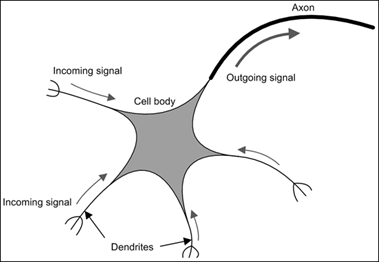
\includegraphics[width=0.6\textwidth]{neuron.png}
    \caption{Simple diagram of a neuron \citep{ScarpinoMatthew2018Tfd}.}
    \label{fig:neuron}
\end{figure}

\break

What they choose to highlight in particular are three points that describe a neuron's functionality 
(see figure \ref{fig:neuron}):

\begin{itemize}
    \item A neuron receives one or more incoming signals and produces one outgoing signal.
    \item A neuron's output can serve as the input of another neuron.
    \item Every neuron has a threshold, and it won't produce an output until the electrical signal
     exceeds the threshold.
\end{itemize}

Perceptrons emulate these features of a neuron.
This page by \citet{anonpercep} highlights a brief history of perceptrons,
serving as a starting point to learn more about the concept. Perceptrons were coined by Frank Rosenblatt in 1961  
\citep{rosenblatt1961principles}. Their research is a bit outdated for this project, therefore a more modern approach
must be identified.

\begin{figure}[h]\
    \centering
    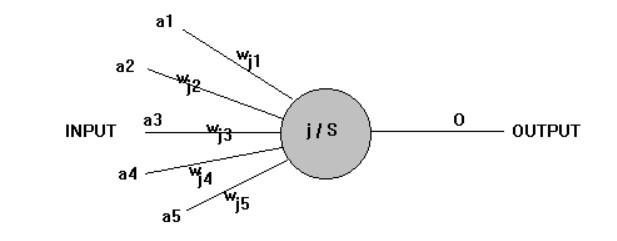
\includegraphics[width=0.7\textwidth]{perceptron.jpg}
    \caption{Diagram of a perceptron \citep{anonpercep}.}
\end{figure}

Each input on the left is weighted and then summed within the circle node. If the summation meets a certain threshold, 
the output will be 1, if it doesn't, then a 0 is outputted \citep{ScarpinoMatthew2018Tfd}. 
Scarpino highlights some 
improvements to the model that were made such as additional biases 
assigned to the incoming signals and an “activation function” that generates the output signal. Scarpino goes further 
by linking activation functions directly to in-built TensorFlow functions that carry out the same task. Making it 
quite useful to understand the link between the TensorFlow API and the underlying DL context. Once 
perceptrons start getting linked together and arranged into layers, a neural network is formed, as seen in figure
\ref{fig:network}:

\begin{figure}[h]\
    \centering
    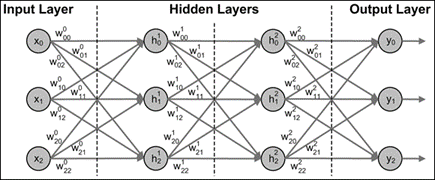
\includegraphics[width=0.7\textwidth]{network.png}
    \caption{Diagram of a layered network of perceptrons \citep{ScarpinoMatthew2018Tfd}.}
    \label{fig:network}
\end{figure}

\section{Convolutional Neural Networks}
\label{subsec:cnn}

\citet{goodfellow2016deep} as well as \citet{ScarpinoMatthew2018Tfd} go into detail about CNNs. Scarpino in particular is a
useful source on how it works with image classification in TensorFlow. However, it's useful to have 
some sort of starting point for the subject. \citet{saha2018} highlights the key features of a CNN and their
purposes such as the individual layers: convolutional (kernel),  pooling and classification (see figure \ref{fig:cnnSimple}).

\begin{figure}[h]\
    \centering
    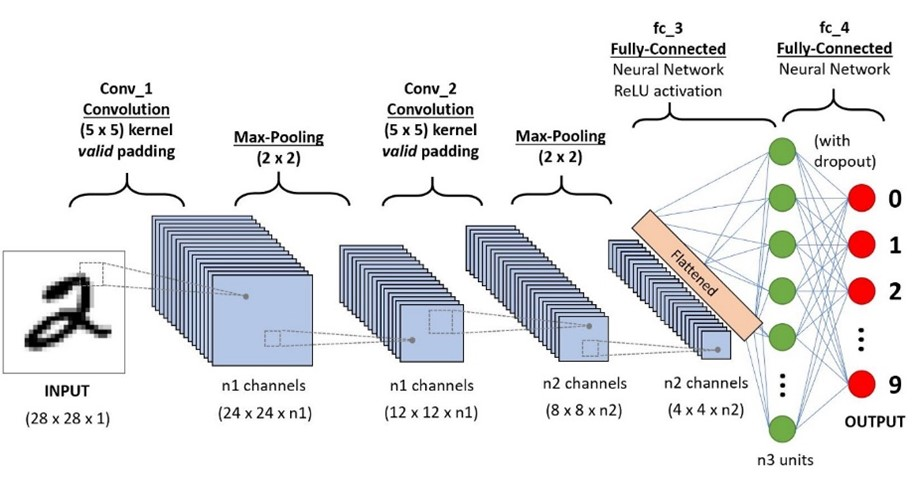
\includegraphics[width=0.7\textwidth]{saha.jpg}
    \caption{Example of a CNN process \citep{saha2018}.}
    \label{fig:cnnSimple}
\end{figure}

They also highlight a feature of CNNs that make images easier to process, where it reduces the size of images,
all while keeping the critical features that are needed for a good prediction. This helps 
with scalability when it comes to dataset sizes in particular. The ELI5 (Explain Like I'm 5) format is 
quite useful and allows us to highlight the key points of each layer \citep{saha2018}:

\begin{itemize}
    \item \textbf{Convolution}: Applying the kernel to extract high and low-level features.
    \item \textbf{Pooling}: Reduces the spatial size of the output from the convolution. Decreases the “computational power” 
    needed for data processing. Additionally, highlights features that are dominant.
    \item \textbf{Classification}: The pooling output is converted into column vectors and fed into a feed-forward neural 
    network where the model is able to distinguish between features and classify them.
\end{itemize}

\citet{saha2018} also highlights that there are actually different implementations of CCNs, therefore they may not function 
in exactly the same format. Dive into Deep Learning \citep{diveintodeeplearning} has a rundown of multiple CNN types 
starting with LeNet-5 and more modern approaches like AlexNet, VGG, NiN, GoogLeNet, etc. They also highlight how to 
implement them using TensorFlow.

\par

\citet{goodfellow2016deep} go into detail about DL from the concept of perceptrons to modern 
implementations. Something they talk about that is interesting, is the increasing dataset and model sizes over time, 
which is quite applicable to the project since smartphone hardware is relatively limited in storage. They discuss how the 
increasing capabilities of computer hardware have led to the development of larger models and that neural networks tend 
to double in size roughly every 2.4 years. They predict that the trend will continue further on in the future. 
Datasets take up storage space and they state that a DL algorithm 
(as of 2015) is expected to perform at acceptable levels with “around 5,000 labelled examples per category, and will match
or exceed human performance when trained with a dataset containing at least 10,000,000 labelled examples". That is of 
course, extremely large and is most definitely going to take up a lot of storage. Therefore, the book does reiterate 
the earlier point of making use of unlabelled data like with semi-supervised learning. \citet{goodfellow2016deep} 
dig deep into the subject of DL and explain areas from applied maths to the modern practices of DL and 
the research in the field. This can prove useful in fully understanding the various processes in place including 
optimisations and ways to increase accuracy that will need to be considered when designing a DL model for the smartphone 
application.

\subsection{ML vs DL}
\label{subsec:mlvsdl}

DL is an obvious evolution from classical ML, but it is worth highlighting the key differences for clarity. 
\citet{kav2020} breaks down how DL is different 
from classical ML. They highlight that DL takes the initiative by automating feature extraction to lessen human intervention and 
that classical ML is more reliant on humans, where they normally define the characteristics to look out for, as well as their 
priorities.

\par

\citet{8359287} go into depth about the key differences when discussing approaches to classical ML and DL in the 
context of cybersecurity. However, the same reasoning can be applied to this project. The key points they highlight 
are:

\begin{itemize}
    \item \textbf{Data dependencies}: DL performs better with larger datasets as well as
    classical ML outperforming DL with smaller datasets.
    \item \textbf{Hardware dependencies}: DL requires a lot of matrix calculations and therefore a Graphical Processing 
    Unit (GPU) can be used to optimise these processes. Note that smartphone hardware does contain GPUs but they are
    not on the same scale as the ones found in some PC hardware. Therefore, it will be interesting to see how DL 
    fares against classical ML when keeping this hardware dependency in mind.
    \item \textbf{Feature processing}: Reiterating on the point mentioned before, DL can extract features directly 
    from the data and requires less human intervention.
    \item \textbf{Execution time}: DL algorithms take a lot longer to train compared to ML, this is dependent on the amount of 
    data.
    \item \textbf{Interpretability}: Because of the complexity of DL, it is hard to determine how a DL algorithm generated a 
    result, whereas classical ML is clearer.
\end{itemize}

The key points have been summarised here, but they go into much more detail which could be helpful when
comparing the two approaches of classical ML and DL.

\section{Flower Classification}

Flower classification is a popular topic in the ML space and this project will outline the challenges and the existing solutions.

\subsection{Existing Methods}

\label{subsec:existing}

Starting with what is known as the “Hello world” of ML, Iris flower classification serves as a simple and easy to 
understand project for developers to implement. The idea is to classify between three classes: Versicolor, Setosa and 
Virginica. There are many tutorials that can be followed online, this particular one by \citet{DataFlairND}
provides additional background information about ML as well as how it will apply to the Iris project which is useful for
a deeper understanding. The tutorial uses the features of sepal length/width and petal length/width to determine the class of
a flower. By using those inputs, they use an SVM to predict the species of a flower with 96\% accuracy.

\par

\citet{Nilsback2008} demonstrate the effectiveness of a multiple kernel SVM on the Oxford Flowers 17 dataset. 
They manipulate the flower data to get key features such as the colour HSV values, the flower texture, shape and 
histogram of gradients (HOG). HOG “captures the more global spatial distribution of the flower” like where the 
petals are arranged. They achieved an accuracy of around 88.3\%. This is impressive considering the key challenges they 
highlight within flower classification. They state that flowers can share a lot of similarities between classes which 
can make it difficult to differentiate between species. Flowers are also “non-rigid objects” and therefore can appear in
many different variations. Overall, they do a good job of explaining their reasoning for their dataset, citing the 
large variety of representations for each flower. They also go into detail about how they extract features from it 
and how to build the classifier.

\par

For DL, there is an extensive study that looks at using transfer learning, which is a technique of retraining
TensorFlow models for different datasets. \citet{Xia2017} use the Inception V3 model to train a classifier for 
the Oxford-17 and Oxford-102 flower datasets. They go into detail about the steps that took place to carry out the 
transfer learning as well as how to reconfigure the last layer of the network to only have 17 and 102 outputs for each 
dataset as it defaults to 1001. They found that the models for the Oxford-17 and Oxford-102 datasets 
produced 95\% and 94\% accuracy respectively. This is a very impressive performance, and their breakdown will be helpful 
when it comes to the implementation produced in this project. 
The paper really outlines the simplicity and flexibility of Google's 
TensorFlow however, it remains to be seen if these great results will translate to a smartphone implementation 
as well.

\subsection{Existing Apps}

A large part of the project is to develop a fully functioning app that uses a
DL model for flower classification. There are existing applications that identify plants in general, as well as
provide other functionality to aid the user that is worth highlighting.

\par

Pl@ntNet is a popular tool that has more than 10 million downloads on the Google Play Store alone \citep{googleplay}. 
It relies on volunteers to validate images and a search engine to identify them. \citet{joly:hal-01182775}
go into detail about the overall experience of the app as well as provide insight into how it works.

\begin{figure}[h]\
    \centering
    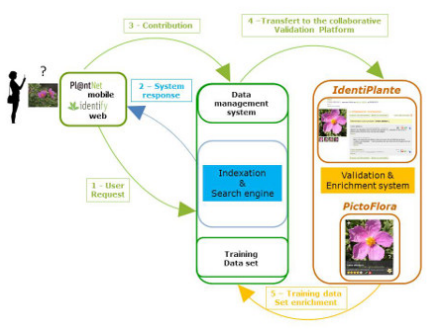
\includegraphics[width=0.7\textwidth]{plantnet.png}
    \caption{Diagram of Pl@ntnet user scenario \citep{joly:hal-01182775}.}
    \label{fig:plantnet}
\end{figure}

Figure \ref{fig:plantnet} shows clearly the type of system in place for the application. The user uses their device to 
query the search
engine and get feedback, their image is also transferred to the collaboration platform if they chose to. It can then be 
independently verified and added back to the training set. The search engine is then retrained on a nightly basis. The 
paper doesn't go into much more detail about the search engine itself apart from mentioning that progress in ML 
and computer vision should improve the performance of identification. Unfortunately, there aren't any new 
papers that provide a better look at the app, so it is hard to understand what changes have been made over the last 
several years as well as what methods they use to build the search engine. There is, however, a dataset now 
available for use that covers over a thousand plant species with over 300 thousand images 
\citep{camille_garcin_2021_5645731}. This is of course out of the scope of the project as it doesn't strictly contain 
flowers, but it does go into detail about how to use the dataset as well as how to load the data and build a model with 
it.

\begin{figure}[h]\
    \centering
    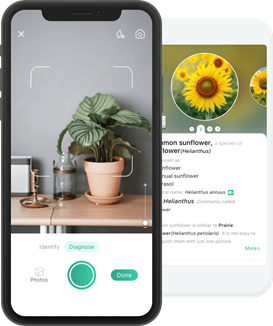
\includegraphics[width=0.4\textwidth]{picturethis.png}
    \caption{Screenshot of PictureThis app \citep{picturethis}.}
\end{figure}

\break

PictureThis is another plant identification app (shown above) that doesn't go into detail about how it works but does 
note that it requires an internet connection to function properly. This suggests that it must communicate with a server 
in order to generate a prediction for images. The app is very streamlined and has an easy-to-use UI that also contains 
useful features such as how to care for the plant and important information about it. The approach used in this project
will be different in 
the sense that any identification process will be carried out on the device however, it is still important to consider 
alternative methods and how they perform so that comparisons can be made.

\section{Evaluation}
\label{subsec:evaluation}

One of the key points of the project is having to evaluate the different classification approaches. This section will
look at the different metrics that are used to rate classifiers.

\par

\citet{10.1145/1163593.1163596} use three performance metrics to test their ML systems: accuracy, precision and recall. 
Accuracy 
is the percentage of correct decisions over the total number of test instances. Confusion matrices can help with 
representing accuracy by providing a “summary of prediction results” where the count of accurate and inaccurate 
predictions are presented per class to show which particular classes the classifier may be struggling with \citep{Brownlee2020b}. 
Precision and recall are a bit more complex. 
Fortunately, \citet{shung2018} demonstrates how these two differ to accuracy. Precision is the number of 
instances that are correctly determined over the total number of instances that are guessed.
 Recall is the number of correctly 
predicted instances over the true number of instances in the class. In addition to these evaluation methods, 
\citet{10.1145/1163593.1163596} outline measuring CPU and memory usage. Fortunately, TensorFlow
contains benchmarking tools to measure: Initialization time, inference time of warmup-state/steady-state and overall 
memory usage \citep{googleTF}. Real-world speeds and accuracy will also be assessed by analysing the app's performance 
during development. The TensorFlow guide also contains tutorials on 
how to choose the best model for the task by comparing model size, accuracy and inference time of different models.
The Lite version of TensorFlow is designed specifically for mobile and internet of things (IoT) 
hardware, so the additional tools will prove useful for the project at the evaluation stage.

\par

\citet{Chockwanich} use the same evaluation methods outlined when comparing different DL models 
implemented in TensorFlow. They also look at CPU usage percentages and processing time. They were able to make a clear 
conclusion of which model is better by evaluating all factors. A term called f1-score was also mentioned in their 
analysis. \citet{shung2018} also explains the relevancy of this metric; it is essentially a way to determine a “balance between
precision and recall”. \citet{kors2021} discusses it further by stating that its purpose is to provide a better 
accuracy statistic that accounts for “imbalanced data”. This means there isn't a good balance of data for each 
class, therefore the classifier makes inaccurate predictions heavily skewed towards classes that there is more data for. 
The f1-score is calculated by:
\[\frac{2*Precision*Recall}{Precision + Recall}\]

\section{Summary}

The review has highlighted the progression of the space from the early concepts to what is known today. 
The area will keep getting more exciting as researchers learn to develop more advanced
algorithms and make use of better hardware capabilities. DL is getting more
accessible as manufacturers allow developers access to their specialised hardware.
Overall, a solid foundation of previous research has been built and it will be interesting 
to see how the field develops in the future. The research that has been conducted will prove useful for the rest of the 
project such as the metrics outlined in section \ref{subsec:evaluation} which will be used to compare the 
two classification approaches that will be investigated.

\clearpage

\chapter{Investigation}

\label{chap:invest}

The main body of this dissertation will be split into two chapters: the first being a comparison
between classical ML and DL using the available Python libraries. The second is 
the design and development of the flower classifier app. This project will start with the investigation portion of the project,
walking through the initial hypotheses, methodology and findings. The idea is to approach this investigation from the 
perspective of a software developer that is analysing the best approach for flower classification to use in 
their product. This includes assessing the quality of the resources available and discussing the possible challenges.

\section{Hypotheses}

The main hypothesis is that a CNN will perform better at classification than a classical ML algorithm. The key metrics 
discussed in section \ref{subsec:evaluation} will be used to confirm this hypothesis. Furthermore, the processes carried
out to implement both approaches and the challenges that were faced will be described. The points outlined in section 
\ref{subsec:mlvsdl} will also be used to promote discussion. 

\section{Design of Experiments}

In this section, the implementation of the classical ML and DL classifiers will be individually described. The results 
from each
approach will then be compared to fully understand the advantages of DL. Furthermore, the development process
including the various challenges faced will be discussed. Firstly, the dataset that will be used will be described.

\subsection{Oxford Flowers 102 Dataset}

This dataset consists of 102 different flower species that occur within the UK. Each class contains between 40 and 258 
images (see figure \ref{fig:dataset_hist}). The images are described to have large variations in scale, 
pose and lighting, even within the classes
themselves. First, the dataset will be downloaded and managed by the TensorFlow Datasets module (TFDS) which will download 
the dataset to a generic directory and can directly manage the image and dataset data including filenames, class names 
and data splits. The data splits defined by TFDS consist of 6,149 images for the test set and 1,020 images for the 
train and validation sets each. This split is atypical as ideally there should be a larger number of images in the training 
set compared to the testing set. The current split is thought to be a mistake on Google's side \citep{githubissue}. As a 
result, the train and test datasets will be swapped to carry out the training process with the larger split which would be 
75\% of the dataset \citep{TFOX102}. Figure \ref{fig:ox102} below shows some of the example images in the dataset.

\begin{figure}[h]\
    \centering
    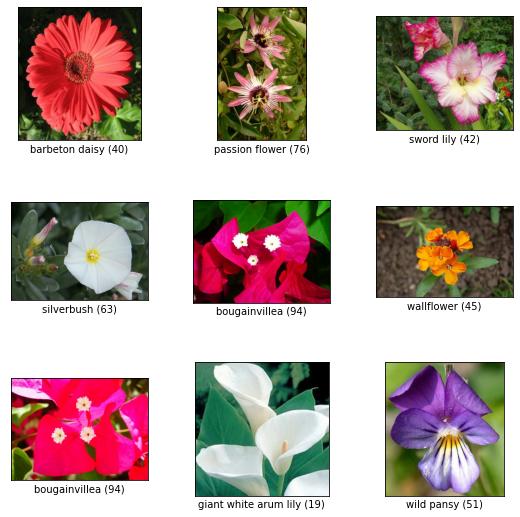
\includegraphics[width=0.7\textwidth]{ox102examples.png}
    \caption{Example images from the dataset.}
    \label{fig:ox102}
\end{figure}

\subsection{Classical Machine Learning}

For this approach, an SVM classifier will be implemented. It will take in features generated using 
“bag-of-words”, HSV (Hue, Saturation, Value) colour values and HOG values. SVM has been shown to have 
good performance with this particular dataset before as 
stated in section \ref{subsec:existing}.

\par

SVMs create a separator between two classes by first plotting data into a feature space of high dimension. The data is 
then transformed so that the separator is represented on a hyperplane. Any new data can then be placed into one of two 
chosen categories that have been separated. The kernel function of the SVM projects data into higher dimensions. 
Depending on the type of kernel chosen, the data could become more “separable” within higher dimensions 
\citep{NobleWilliamS2006Wias}. The default kernel, Radial Basis Function (RBF) will be used \citep{sckikitsvm}. 

\par

A value of 98.5\% accuracy has also been achieved by using a CNN to extract the features 
\citep{mete}. A CNN will not be used to extract the features in this approach as the purpose of this investigation is to 
evaluate both 
approaches separately instead of combining aspects from both. Bag-of-words will be used as it is simple to implement, 
but will also provide consistent information about key points found in the image, despite how the image is presented in 
terms of factors like rotation and scale \citep{mohan}.
The “words” will be produced by extracting key points using Scale Invariant Feature
Transform (SIFT) and then clustered by a K-Means trainer using 200 clusters to make up the “vocabulary”. HSV values are 
useful as they give
the relevant colour data as well as information about the 
luminance in the image \citep{chapelle1999support}. HOG values provide information about the general
shape of the object; this is useful in mapping the various shapes and sizes that flowers come in. The dataset images 
will be resized to have a height and width of 
299 pixels to match the input image conditions of the DL approach. All SVM parameters will be set to the 
default that is defined by the documentation.

\subsection{Deep Learning}

The CNN used in this approach will be Inception V3, a pre-trained network, specifically trained on the iNaturalist 
dataset, which contains 675,170 training and validation images from 5,089 categories \citep{paperswithcode}. 
This means that the model has been optimised for recognizing plants and animals which makes it the best candidate to be 
used for transfer learning to allow it to recognize flower species. It is also listed as the second-best model hosted on
TensorFlow. Inception V4 exists and has a better performance compared to V3 but there are no fine-tuneable V4 models available.   

\begin{figure}[h]\
    \centering
    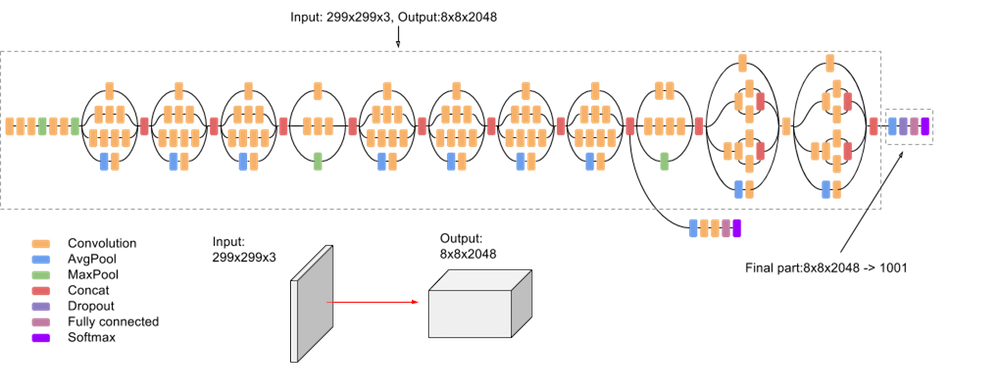
\includegraphics[width=\textwidth]{inceptionv3.png}
    \caption{The Inception V3 model diagram \citep{GoogleCloud}.}
    \label{fig:inception}
\end{figure}

Compared to the initial research of DL models presented in figure \ref{fig:cnnSimple} within the literature 
review, figure \ref{fig:inception} demonstrates how complex they can truly be. 
The terms convolution and pooling within section \ref{subsec:cnn} were already discussed however, there are additional 
layers here that were not discussed:

\begin{itemize}
    \item \textbf{Concatenate (Concat)} takes a list of tensors and outputs a single combined tensor \citep{kerasconcat}.
    \item \textbf{Fully connected layers} map all inputs in the previous layer to every “activation unit” of the layer next to it
\citep{singhsurya}.
    \item \textbf{Softmax} is where probabilities are assigned to each label based on the likelihood of the image belonging to 
that label. All probabilities add up to 1 \citep{googledevcnn}. 
    \item \textbf{Dropout} mitigates the overfitting of a dataset by randomly dropping out neurons on each pass of the network when 
    training \citep{seb}. 
\end{itemize}

The images will go through some data pre-processing such as resizing to have a width and height of 299 as that is the 
requirement of the input tensor for Inception V3. A tensor is an immutable data structure that consists of multi-dimensional
arrays that will store the image data in this case \citep{tensor}. They will also have to have their values rescaled from 0-255 to 
between 0-1. Random flips and crops will also be added as part of the pre-processing pipeline. Images will be batched 
into sets of 32, this means that 32 images will be trained per step per epoch. 

\par

Transfer Learning will be used to retrain the model for this dataset. This is where a developer can make use of the
pre-trained model's feature maps without having to retrain the whole model from the beginning. By using the 
“fine-tuning” option, re-training can be done at a larger scale within the model by unfreezing some of the top layers, 
this can make the model better at classifying images in a particular dataset. Otherwise, these layers will 
remain frozen and only the final layers will be retrained \citep{transfer}. Some additional layers will be added to the 
sequence, the 
first is a dropout layer to prevent overfitting and then a softmax dense layer to reduce the number of outputs from the default 
to 102 so it matches the number of classes in the dataset \citep{denselayer}. Each output will be the probability of an 
input image being a
certain class. Activating fine-tuning will increase the number of trainable parameters from 208,998 to 21,977,350 which 
will significantly increase training time; therefore, it is worth looking into whether this trade-off is beneficial in 
any way.

\par

Hyperparameter tuning is also 
required to try and get the best performance possible. These are the hyperparameters that will be adjusted and
their supposed effect:

\begin{itemize}
    \item \textbf{Optimiser} is used to improve the speed and performance of the model by adjusting the parameters of the 
    model during training to minimise loss and maximise accuracy \citep{maithani}. The types of optimisers that will be
    tested are Adam, Stochastic Gradient Descent (SGD) and AdaMax. There are a few more optimisers 
    available that are not listed, as they are unsuitable for this dataset.
    \item \textbf{Learning rate} is the rate at which a model learns, a larger value means that the model learns faster 
    at the expense of producing substandard weights for the model \citep{andreaperlato}. Values from 0.01-0.0001 will
    be tested, moving down a magnitude at each step. 
    \item \textbf{Dropout}, which was described earlier when discussing the Inception V3 model. Increasing this value 
    will mean a larger percentage of nodes will get removed. Values within the range 0.2-0.4, in increments of 0.1 
    will be tested.
\end{itemize}

Using a TensorFlow module called TensorBoard, the different hyperparameter combinations can be tested to produce the
performance
metrics for each combination. TensorBoard allows the developer to view how the hyperparameters affected the results. 
In an effort to decrease overall training time, some preliminary testing will be conducted to see which 
optimiser is more suitable with just baseline parameters. Once that is selected, only the different 
learning and dropout rates need to be tested using a \emph{grid search}. This is when every possible parameter combination is tested 
\citep{gridsearch}. 
When testing with a 
large number of hyperparameters, one can use other methods like random search to decrease overall tuning time by 
randomly sampling hyperparameters from a range based on a statistical distribution. This means that more effective 
hyperparameters are tested to avoid spending time on one that will not affect the overall performance that
much \citep{sayak}. 

\subsection{Environment}

\label{subsec:env}

Both approaches will be developed and run on the same machine, a custom desktop PC that contains these main components: 

\begin{itemize}
    \item An AMD Ryzen 3600 4.2Ghz 6 Core/12 Thread CPU
    \item 16GB 3200Mhz DDR4 Memory
\end{itemize}

The PC ran on Ubuntu 20.04 LTS with the relevant Python and TensorFlow libraries needed to run the Jupyter Notebooks 
locally. VS Code was used as the Integrated Development Environment (IDE) with the Python and Jupyter extensions.  It is
possible to run model training on the GPU instead of the CPU, however, only Nvidia GPUs are directly supported. As a 
result of not having access to one for this project, the CPU will be used to carry out training.

\subsection{Metrics}

The key metrics that will be analysed along with accuracy, precision, recall and f1-score are: 

\begin{itemize}
    \item \textbf{Loss}: A measure of how bad the model's predictions are \citep{googletrainloss}. 
    This metric only applies to the DL approach as it is calculated during the training process as the model 
    tries to minimise it.
    \item \textbf{Area under the receiving operating characteristic curve (AOC)}: Computed by plotting the true-positive
    rate against the false-positive rate. The area under this curve indicates how well the model performs at selecting 
    the correct prediction against all other predictions \citep{googleroc}.
\end{itemize}

\section{Results}

In this section, the results of the approaches will be presented and discussed, starting with what was found during the
initial testing phase of the DL implementation.

\subsection{Hyperparameter tuning}

Another factor to consider when carrying out training is the number of epochs. An epoch is a full pass over the training
set \citep{epoch}. Multiple passes are needed to minimise loss and fully train the model. Through preliminary testing 
of the model, 
it was found that 5 epochs are more than sufficient as the maximum accuracy is reached, as shown in figure 
\ref{fig:incep_acc}. If
the number of epochs is increased, there is a risk of overfitting \citep{geeksforgeeks}. Optimisers were tested individually to 
determine how much they would affect the results under standard conditions. SGD was found to be unsuitable for this 
task, producing accuracy results at almost half of what Adam and AdaMax were producing. Overall, Adam produced the best 
results, with AdaMax being only a percentage point behind. Therefore, it was decided to conduct any main hyperparameter 
tuning, purely using the Adam optimiser. All hyperparameter tuning is done to only the first epoch to reduce overall 
execution time. 

\begin{figure}[h]\
    \centering
    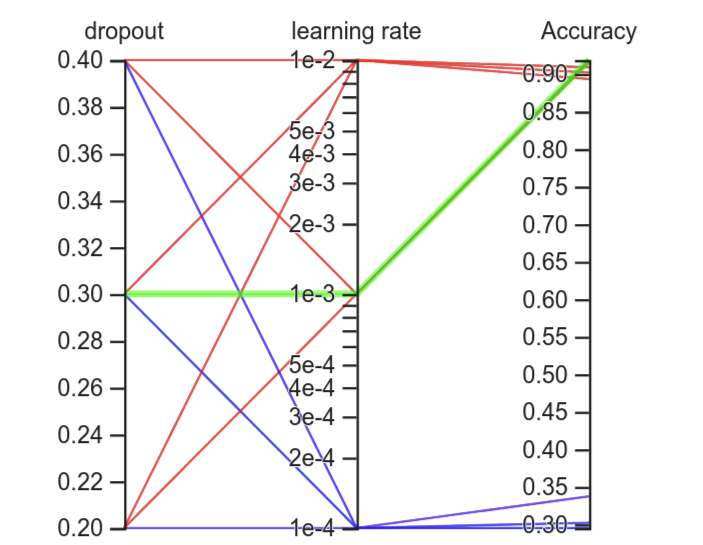
\includegraphics[width=0.6\textwidth]{cross_graph.png}
    \caption{Graph generated in TensorBoard from HP training results.}
    \label{fig:cross}
\end{figure}

\break

Figure \ref{fig:cross} above is a parallel coordinates view shown within TensorBoard that clearly outlines what accuracy 
results 
certain combinations of hyperparameters produce. Highlighted in green shows the joint first highest with a dropout of 
0.3 and a learning rate of 0.001. A dropout of 0.2 with the same learning rate produces the same result. A learning rate
of 1e-4 produces a significant reduction in first epoch performance, this is because the number of overall epochs would
need to increase to account for the slower learning rate \citep{lrate}. Ideally, it would be best to test the number of epochs along 
with the other 
hyperparameters to produce fairer results, however, that would significantly increase training time with a grid search. 
If a developer has access to more specialised hardware, suited for these tasks, this would not be too much of
an issue.

\par

Overall, the final model will use a learning rate of 0.001 and a dropout of 0.3. This was decided after considering the 
results from the hyperparameter tuning (Appendix \ref{subsec:hp}) as well as the proposed learning rate being the 
default one provided by the TensorFlow API. Fine-tuning was also considered, however after some test runs, it was
determined that increasing the number of trainable parameters, increases the memory usage of the program significantly.
As a result, the program would fail to execute as the system memory limit would be exceeded 
(see figure \ref{fig:finetuning}).

\subsection{Performance}

Here are the overall performance metrics produced from both approaches:

\begin{table}[h!]
    \centering
    \begin{tabular}{ |l|l|l| }
        \hline
        Metric & SVM (\%) & Inception V3 (\%) \\
        \hline
        \hline
        Accuracy & 24.30 & 95.69 \\
        \hline
        Loss & - & 17.95 \\
        \hline
        Precision & 29.40 & 96.14 \\
        \hline
        Recall & 24.30 & 95.69 \\
        \hline
        F1 & 26.60 & 95.91 \\
        \hline
        ROC AUC & 89.60 & 99.97 \\
        \hline
    \end{tabular}
    \caption{Results output from the classifier after predicting against the testing dataset.}
    \label{table:2}
\end{table}

\break

Precision, recall and ROC AUC values are weighted, meaning that they consider class balance as they calculate the metrics
for each class and find the average weighted by the number of correct instances for each class 
\citep{scikitprec}. This was necessary, to account for the slight imbalances in the number of images 
in each class. The DL approach clearly comes out on top with excellent results.

\par

The Inception V3 test contains additional information about accuracy (figure \ref{fig:incep_acc}) and loss 
(Appendix \ref{subsec:loss}) for the training and validation datasets 
while the model is being trained. It demonstrates how the model improves per epoch.

\begin{figure}[h]\
    \centering
    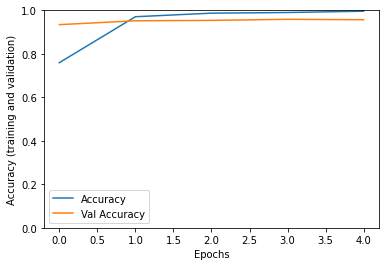
\includegraphics[width=0.6\textwidth]{Accuracy.png}
    \caption{Graph of accuracy against the number of epochs.}
    \label{fig:incep_acc}
\end{figure}

The model needs to be converted to a TensorFlow Lite file in order for it to be used in the Android 
application. Once it is converted, the model can be reloaded to run inference on it, to check if it is still effective. The 
result after doing that produces an accuracy of 100\% if it is tested on just the first batch of 32 images. Of course, 
this is not indicative of real-world performance, and additional performance profiling will be conducted
once the app is developed. 

\section{Analysis}

In this section, the results will be analysed in more detail. A comparison of both approaches will also be made here
to get a better understanding of the advantages of DL.

\subsection{Outcome}

It is clear that the DL approach is vastly superior in classifying flowers to the SVM in all aspects. The Inception V3
approach has high accuracy, meaning it can correctly identify the classes of most of the images in the test set. 
High precision indicates that a large portion of correct identifications were genuinely correct. High recall demonstrates
how well the classifier identified correct instances. One might notice that accuracy and recall are the same value for 
both classifiers, this is because they represent the same thing in non-binary classification. Recall is shown to be:

\begin{equation}
    \frac{TP}{TP+FN}
\end{equation}

Where \(TP\) is number of true-positives and \(FP\) is the number of false-negatives \citep{googledevrecall}.

\par

In this case, FN is every incorrect evaluation of a class. Therefore, by calculating the recall value for each class,
it is essentially tallying up the number of times the class has been correctly identified over the total number of 
images in the class, for every class, giving the same calculation as total accuracy. F1 gives a better indication of 
the accuracy of 
the classifier, by taking into account the precision and recall, the high f1-score indicates that even with class 
imbalance, the classifier performs well. An AUC of near 100\% means that the predictions are nearly always 
correct. The other predictions of an image are taken into account, so while the classifier might choose the incorrect 
overall label, if the true label has a high probability, the classifier is still somewhat good at 
identifying the correct label.

\par

The SVM falls behind in every aspect, therefore, it is not worth pursuing as a method for flower classification in this 
dataset. It is still possible to adjust the parameters of the SVM to get better performance or get more feature data 
from the feature extraction methods. The current implementation, specifically the histogram calculations, uses parameters
that decrease extraction and training time significantly, in exchange for outputting less information. 
\citet{Nilsback2008}
achieved an accuracy of 88.3\% with the Oxford Flowers 17 dataset, a smaller subset of the one being used here using 
very similar methods of combining SIFT, HOG and HSV. Their method is a lot more intuitive than this SVM
implementation but still doesn't reach the performance of the Inception V3 model. This doesn't mean that SVM or any 
other classical ML method is obsolete, even in being used as a classifier on smartphones. They can still
perform extremely well on smaller and less complex datasets. Therefore, if dataset complexity is not an issue, what 
else is there to consider? The ease of implementation and how easy it is to move the classifier 
into a smartphone can be looked at.

\subsection{Comparison of Development Processes}
Most of the SVM was implemented with the help of Scikit which contains easy to understand documentation on how to 
implement an SVM as well as many other ML algorithms. There is also example code that gives developers an 
idea of how to implement the algorithms in Python. Scikit provides a more extensive support library for hyperparameter 
tuning compared to TensorFlow, including in-built functions for a grid search. TensorFlow uses TensorBoard as a platform 
to display the results of tuning as well as the overall results of training, which is very useful but doesn't provide 
any additional API level support for finding the right hyperparameters. That is up to the developer to implement it 
themselves. Scikit provides additional tools to allow model persistence so that developer trained models can be saved 
and reused later. However, allowing these saved models to be used within an android application doesn't appear to be 
straightforward compared to the TensorFlow approach and there does not seem to be any documentation to help with this. 

\par

The documentation for TensorFlow is extremely robust. This is unsurprising, considering it is developed and maintained 
by Google. There is a clear-cut development process for the developer, where a beginner, can understand the basics and 
go on to develop and train their first neural network on any of the supported platforms. The Keras Python API runs on 
top of the TensorFlow platform and is designed to be easy for developers to use and produce results quickly 
\citep{kerasabout}. The approach used here involved adapting the example code provided in the TensorFlow API. This allowed
for the quick development of a working example that could be adjusted by simply searching through the API documentation. The 
documentation is easy to follow as it provides clear explanations as well as examples of how it would be used. The 
process to train models for different datasets using transfer learning is simple as well, allowing developers to adapt most
models. A model can be saved to storage so that it can be reloaded, and re-training is not required. The saved 
model can then be converted to be used as a TensorFlow Lite model, so it can be integrated into a smartphone app. 
The process for this
is simple and requires using the example code provided, to implement. The developer needs to provide the 
details to describe the model, including the shape of the input tensor, the image data type, and the number of classes. 
This data can then be used by the TensorFlow Lite interpreter within Android.

\subsection{Summary}

This investigation has been very educational and has certainly shown the capabilities of these specially made software 
libraries. It is worth going back to discuss the main differences between ML and DL discussed in section \ref{subsec:mlvsdl}
and see if they 
still hold. Data dependencies are first discussed, and it is certainly impressive how well Inception V3 handles the 
Oxford Flowers 102 dataset compared to the SVM. The model is capable of handling datasets that contain up to 1001 
classes, therefore, it is possible to push the model even further. It would've been interesting to see how effective a 
GPU would be with training so that comparisons could be made on how much of an improvement it is over just using a CPU. 
The DL approach certainly required less set-up and thought when it came to actually implementing a classifier. This is 
because the model can directly extract features and the developer doesn't have to worry about what features to extract 
as they do with an SVM. The training time is about the same for both approaches. When increasing the number of 
features produced from the bag of words, HSV and HOG extractors, the training time would also increase significantly. 
Similarly, with the DL model, when decreasing the learning rate and adding more epochs.
Therefore, that comparison is situational. When it comes to understanding the functionality of the two approaches, it 
was certainly a requirement to understand the SVM approach relatively in-depth compared to the DL approach. This is 
mainly because of the feature extraction process, where developers can clearly see what exactly is being analysed and 
the exact format of the input data. Whereas, with DL, it appears to be more like a black box, where the complexity of 
the model is abstracted away from the developer. Therefore, the only requirements were to provide the data in the format
expected for the model to function properly to get results. TensorFlow has shown itself to be a 
very capable library that allows developers to easily implement DL for many use cases and it is exciting to see
how it will improve in the future. 


\clearpage

\chapter{Flower Classification App}

The second part of the main body involves designing, implementing and testing an Android app that can recognise flower
species. The TensorFlow library will be used to seamlessly integrate the DL model developed in chapter
\ref{chap:invest} into an app. Then, the various processes that will take place, challenges faced and real-world 
performance of the final product will be discussed.

\section{Requirements and Specification}

\label{subsec:req}

Requirements were defined based on the findings produced in the literature review. This includes the background research 
related to the goals of DL and the findings from the review of the existing solutions. The 
guidelines produced by Google when it comes to TensorFlow integration, Material You design and Android development will be used. 
These are useful in designing and developing applications that conform to the general Google standards. As there is
no defined client or target market, there are no requirements based on questionnaires and interviews. 
Therefore, the aim is to describe the development process and test the performance of the app so that the feasibility of 
using DL within a smartphone can be assessed. 

\subsection{Literature and Technology Survey Findings}

The Literature and Technology review walked through the evolution of the domain and how DL was the product of many years
of research and development. It is important, to re-iterate the reason why there is a large number of resources 
dedicated to the progress of this space. The goal is to imitate human-like decision making within a computer. In the 
context of flowers, this means the ability for a computer to recognise different flower species accurately and 
efficiently. This means that the system must be able to recognise the flowers correctly and in a timely manner.

\par

Pl@ntNet is the most robust existing solution reviewed in this project with a system that can identify a large number of 
different plant species. Due to the many different categories of plant life that the app supports, the user interface 
uses additional settings to narrow the search. The process of taking a picture and then getting the results is quite 
simple however, they are carried out within separate views.  This means that taking a picture, viewing the picture that 
was taken afterwards and then getting the results, all occur in different views. This process can be simplified
by keeping this three-step process within a single view. The app also shows the different percentages for the 
different estimates it has on the results page. This is a useful feature as it can show the user alternative 
guesses if the classifier makes an inaccurate or unsure suggestion. To summarise, the system should contain a
simple classification process that provides adequate result information to the front end such as the probability 
percentages. 

Different types of implementations were also discussed within the review such as cloud-based or on-device. 
The PictureThis app used a cloud-based implementation that requires network connectivity in order to function. 
The obvious downside to this is that it won't work offline, and network latency will have to be taken into account when 
the classification process occurs. The flower classification app aims to be fully functional offline by having the model
stored on the device. Fortunately, because of the advancements in smartphone hardware, model sizes that may be over 100MB 
in size are acceptable, which means more accurate models can be stored.

\subsection{Google Developer Practices}

\subsubsection{TensorFlow}

The guidelines to transfer a saved model will be followed. This involves training using the TensorFlow API and then
converting it into a TensorFlow Lite model, 
designed for usage on a smartphone. The Inception V3 model that has been trained and tested in chapter \ref{chap:invest}
is a 
floating-point model, which means that GPU acceleration can be used in order to decrease inference time 
\citep{TFGPU}. The documentation also provides additional advice on tuning the interpreter to get the best 
performance. Android Studio, the main IDE used by Android App Developers has tools that can help analyse the 
real-world performance of the interpreter, which will be key during the development process. By following the advice 
given by the documentation, key areas of optimisation within the app can be identified. 
Areas that will be considered are performance on the GPU and the performance using the CPU with varying numbers of threads.

\subsubsection{Android Developers}

Apart from general UI interactions like button presses and UI updates, the only additional library support that needs to 
be considered from the Android platform is the camera API. The camera plays a big part in the classification process as it 
provides the input image information for the model. The application will make use of the newest CameraX API which is 
designed to be easy to use and have support for the majority of Android devices including legacy devices down to Android 5 
\citep{ADCameraX}. Using this API, developers can control the input image dimensions and provide image previews to the 
user.

\subsubsection{Material You}

This is a secondary objective, but conforming to the latest Google UI standards may prove beneficial in creating 
an easy-to-use UI. Material You is the latest iteration of Android's design language with an emphasis on helping “make 
technology simple and beautiful for everyone” \citep{material}. Since the app revolves around capturing flowers, widely 
regarded as beautiful objects, having a simple and pleasing UI seems appropriate. 

\subsection{Functional Requirements}

The requirements table can be seen in Appendix \ref{subsec:funcreq}. It is worth elaborating on them to get a clearer 
picture of how the final product will function. 

\par

Firstly, the app must run on Android devices of minimum API level 26. This is Android version 8.0 and 
consists of approximately 82.7\% of devices (Appendix \ref{subsec:sdk}). 
There are possible ways to make an app that works for iPhone by using Google's Flutter development kit that allows 
for deployment to both ecosystems and compatibility with TensorFlow. However, due to the inability to access an iPhone 
to test the app, it is best to proceed with an Android-only implementation.

\par

Through the use of the CameraX API, the app must be able to capture and display images. The camera viewfinder will be 
visible to the user. When a picture is captured, the view will transition to showing the image that was captured so 
that the user can clearly see the quality of the image they have captured and whether the subject of the image is in 
full view.

\par

The app must integrate the Inception V3 model trained in chapter \ref{chap:invest}. 
This model will allow for the classification of 
images captured in the app. The output information which includes the classification results and their percentage 
probabilities, will be parsed and outputted to the front end.

\par

Results produced by the app must be shown in an acceptable time frame after capturing the image. It is not ideal for 
the user to have to wait for a long period of time to get the results. An inference time of less than 
half a second should be acceptable. This falls in line with the estimated times defined on the TensorFlow site which can also 
be seen in Appendix \ref{subsec:models}. Within this time period, the app must also display the top three predictions 
to the front end. 
If the classifier is unsure about the label of the input image, the user can at least see what other possible labels it 
could be. The predictions will be shown in a clear order from best to third-best prediction. A small thumbnail image of 
the flower should also accompany the label in the UI so that the user can see if the flower they have captured matches 
up with the prediction, in case they're not sure of whether the predicted label is correct. 

\par

To track if the classifier is recognising images in an acceptable time, an element will be shown within the UI that outputs 
how long it took from the picture being taken to the image being classified.

\subsection{Non-functional Requirements}

A table of non-functional requirements is also defined in Appendix \ref{subsec:nonreq}.

\par

The app should function with minimal bugs so that the overall experience of using the app is not hindered by unintended 
behaviour or crashes. It will also make sure testing of the app's performance goes smoother. If there are crashes or 
bugs it will mean the testing results are less reliable.

\par

The app will be designed around the Material You design specification which involves producing simple and intuitive user
interfaces that conform to the latest Google standards. The aim is to make the app simple to use and not involve too 
many background UI processes so that the classification process is not hindered in any way. 

\par

\section{Design and Implementation}

This section will consist of the design and implementation process of developing the flower classifier app. 
The objective is to follow the requirements outlined in section \ref{subsec:req} to produce the app, but first, a plan 
must be outlined to ensure development goes smoothly.
 
\begin{figure}[h]
    \centering
    \begin{tikzpicture}
        \node[draw,
        rounded rectangle,
        minimum width=2.5cm,
        minimum height=1cm] (block1) {START};

        \node[draw,
        minimum width=1cm,
        minimum height=1cm,
        right= of block1] (block2) {Locate flower};

        \node[draw,
        trapezium, 
        trapezium left angle = 65,
        trapezium right angle = 115,
        trapezium stretches,
        right=of block2,
        minimum width=3.5cm,
        minimum height=1cm
        ] (block3) { Capture image };

        \node[draw,
        minimum width=1cm,
        minimum height=1cm,
        right= of block3] (block4) {Classification};

        \node[draw,
        trapezium, 
        trapezium left angle = 65,
        trapezium right angle = 115,
        trapezium stretches,
        below=of block4,
        minimum width=3.5cm,
        minimum height=1cm
        ] (block5) { Results };

        \node[draw,
        diamond,
        below=of block2,
        minimum width=3cm,
        inner sep=0] (block6) { Clear image? };

        \node[draw,
        rounded rectangle,
        minimum width=2.5cm,
        minimum height=1cm,
        left= of block6] (block7) {END};

        \draw[-latex] (block1) edge (block2);

        \draw[-latex] (block2) edge (block3);

        \draw[-latex] (block3) edge (block4);

        \draw[-latex] (block4) edge (block5);

        \draw[-latex] (block5) |- (block6);

        \draw[-latex] (block6) edge node[pos=0.45,fill=white,inner sep=2pt]{No}(block7)
        (block6) edge 
            node[pos=0.4,fill=white,inner sep=0]{Yes}(block2);


    \end{tikzpicture}
    \caption{Flowchart that shows the actions that need to take place to classify a flower in the app.}
    \label{fig:flow}
\end{figure}

\par

\subsection{Classifier}

The Inception V3 model has a set of requirements that need to be filled in order to function. This is where using the 
TensorFlow and CameraX guidelines is important as it needs to be determined if these pieces can work together. 
The classifier expects 
an object named \emph{TensorImage}. This object requires the loading of a bitmap image in order to be valid. This means that
some pre-processing must be carried out to convert an image into a bitmap, to then load the bitmap into a \emph{TensorImage} so it can 
 be resized to have a height and width of 299 by 299 as required by the model.  The image may also need to be rotated
as the raw image from the camera sensor is not normally in the orientation a user would expect.
Figure \ref{fig:classify} outlines the full process that needs to be carried out to classify a raw image.

\begin{figure}[h]
    \centering

    \begin{tikzpicture}

        \node[draw,
            minimum width=1cm,
            minimum height=1cm,
            ] (block1) {Raw Image};

        \node[draw,
            minimum width=1cm,
            minimum height=1cm,
            right=of block1
            ] (block2) {Bitmap};

        \node[draw,
            minimum width=1cm,
            minimum height=1cm,
            right=of block2
            ] (block3) {Tensor Image};
        
        \node[draw,
            minimum width=1cm,
            minimum height=1cm,
            right=of block3
            ] (block4) {Resized and Rotated};

        \node[draw,
            minimum width=1cm,
            minimum height=1cm,
            right=of block4
            ] (block5) {Classifier};

        \draw[-latex] (block1) edge (block2);

        \draw[-latex] (block2) edge (block3);

        \draw[-latex] (block3) edge (block4);

        \draw[-latex] (block4) edge (block5);

    \end{tikzpicture}
    \caption{Diagram that shows the processing an image has to go through until it gets fed to the classifier.}
    \label{fig:classify}
\end{figure}

\subsection{Implementation Process}

The environment is the same as what was described in section \ref{subsec:env}. The key difference is that the Android 
Studio IDE will be used for the development of the app. Testing will take place directly on a Samsung Galaxy S20 5G. 
This device is one of the flagship Samsung phones released in the year 2020 and has decent specifications for a 
smartphone. The exact specifications can be seen in Appendix \ref{subsec:phone_spec}. Android Studio has an in-built 
tool that can easily process TensorFlow Lite files that have the extension “.tflite”. By using the tool, the relevant 
app directories are created for the developer, as well as the library dependencies to use TensorFlow.

\subsection{User Interface Design}

While this is not relevant to the base functionality of the application. It is still important to plan a user interface 
that will allow the user to carry out the simple operation of classifying flowers on their device. Therefore, some rough
sketches were produced to plan out the single view that will encompass everything, including the camera and results interface as 
seen in figure \ref{fig:sketch_main}. There is also an additional view as seen in figure \ref{fig:sketch_info} that outlines a description page for the 
flowers.

\begin{figure}[h]\
    \centering
    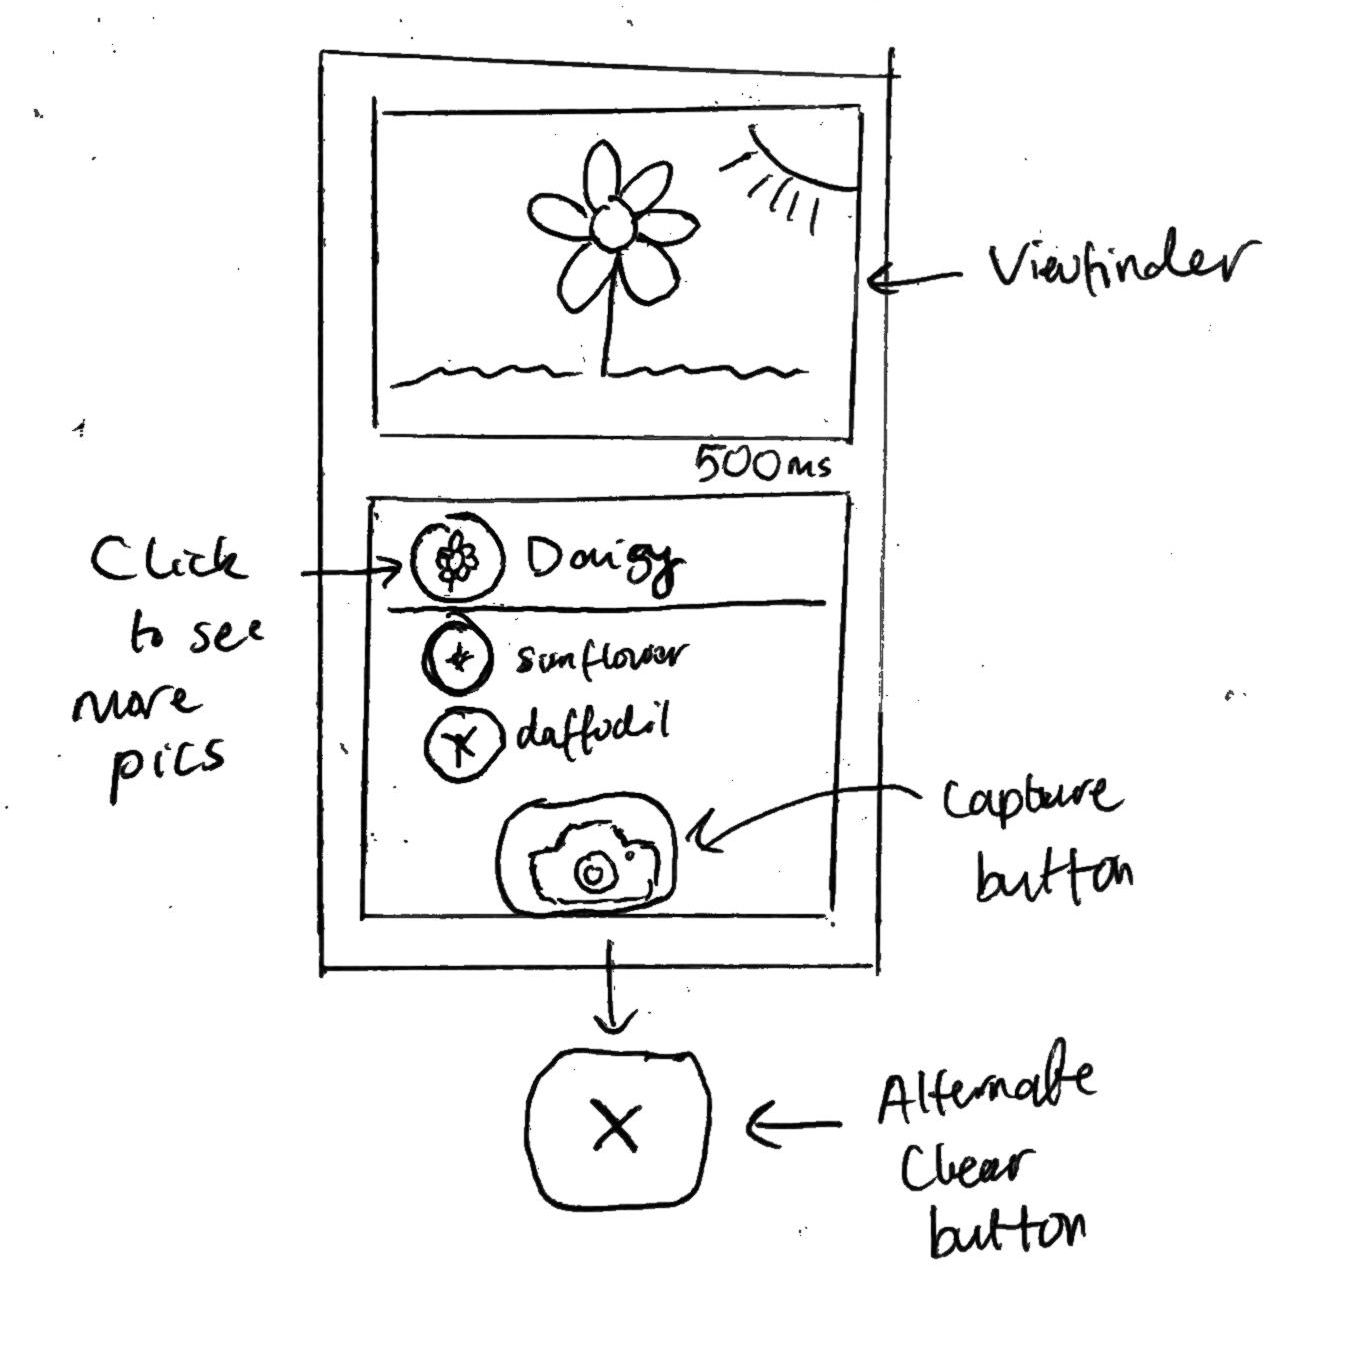
\includegraphics[width=0.6\textwidth]{Main_Sketch.jpg}
    \caption{Sketch of the home page.}
    \label{fig:sketch_main}
\end{figure}

The home page's main purpose is to capture the flower image and provide the results to the user. The sketch provides 
that simple outline to follow when designing the interface within the IDE. The viewfinder box at the top should take no 
more than half the screen to leave enough room for the classification results. There are three rows for the top three 
results however, the top row is slightly bigger to highlight the top result more than the others. Images for each result
are included to help the user see what the predicted flowers actually look like.

\begin{figure}[h]\
    \centering
    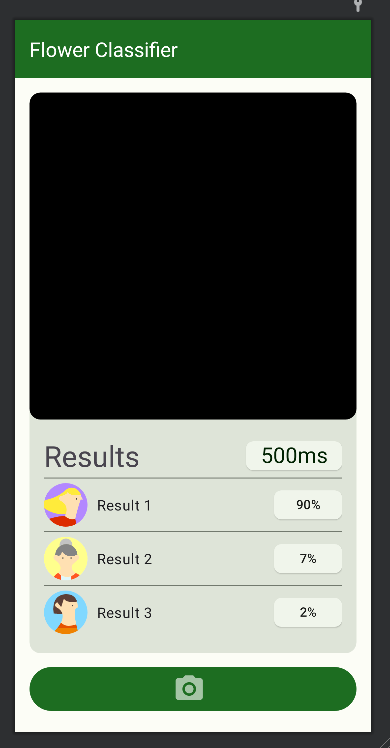
\includegraphics[width=0.3\textwidth]{IDE_Ver.png}
    \caption{IDE preview of the home page.}
    \label{fig:final_des}
\end{figure}

\break

Figure \ref{fig:final_des} shows the final version of the design that was made within the IDE. It follows the general 
layout given by 
the sketch. There are some minor changes with the sizing of some elements to make them stand out more like the camera 
button. Also, the result elements are all uniform in size to make the image icons clearer. Overall, the design consists 
of all Material You elements which were located and sized based on the guidelines given by Google. 


\section{System Testing}

There are two main aims for the testing portion of this section. The first aim is to ensure the base 
functionality is working as intended through functionality testing. To show this, some real-world examples of the app 
identifying various flowers will be demonstrated. Once, the app is established to be working as intended, the next step will be to carry out 
performance testing to see how the classifier is performing within the app. By using performance profiling, there can be a focus
on specific work threads where the classifier is carrying out the identification process. Certain factors 
like whether to use the GPU or CPU as well as the number of threads to dedicate to the classifier will be altered. Then,
the results will be discussed. Before testing takes place, the phone will use the in-built system clean up tool that 
clears any unnecessary background apps and processes.

\subsection{Functionality Testing}

This will be split into two formats. The first is to try and identify as many different flowers that are available 
and report the probabilities for the top three labels as well as the inference time when the app is working on the GPU. 
The second format is to analyse how the app performs using the same metrics but with the same flower, shot at different 
angles.

Appendix \ref{subsec:functionality} contains the results of identifying eight different flower species found in the 
vicinity. All of them bar 
one have a confirmed species. There are also screenshots that go with each result within the Appendix where one can view 
the exact angles and lighting conditions the photos were taken in as well as what the other predictions are, for that 
flower. The results show that six of the species have been correctly identified by the classifier. There are five 
species within that selection that have probabilities of 88\% and above, each of these flowers are very common in 
the UK and have distinctive shapes and colours. This suggests the classifier performs very well with these unique 
flowers, most likely as they don't have too much of a shape and colour crossover with other species. The classifier also
works well in identifying the two different dandelion types. These flowers are very different in appearance but are 
still both dandelions. In the case of the flower identified as a Columbine, it is unconfirmed whether the subject 
flower is in fact a Columbine, but by looking at some of the example flowers in the dataset, it is clear why the 
classifier came to that conclusion. The orchid that is incorrectly identified as a Cyclamen has a second guess of 
Sweat Pea that is also 47\%. This suggests that the classifier cannot make a definitive decision of what the flower is,
likely due to a lack of orchids within the dataset. Moon orchids are a class within the dataset and are not too 
dissimilar in appearance to this orchid \citep{PlantsState}. Therefore, it is unclear as to why that class was not 
suggested over the other classes. Subsequent classification attempts on this same plant yielded consistent high 
probabilities for the Cyclamen class, suggesting it didn't matter what angle the picture was taken in. The inference 
times seem consistent using the GPU. It will be interesting to see what the performance will be like when using the
different hardware configuration types.

Some additional testing was carried out on the same rose to see how the classifier dealt with different angles and 
lighting conditions. The first set of tests will include classifying with different camera distances and angles with 
estimated measurements. The first was the distance test where multiple shots of the same rose were taken. The camera
was angled to have the centre of the rose in the middle of the viewfinder. The rose was always in the same position and 
location to keep the lighting consistent. The results from this experiment are presented in Appendix 
\ref{subsec:distance}. The distance appears to have an effect on the classification accuracy. The prediction at 4cm has a 
low probability of 39\% but still,
ranks rose as the most likely. This indicates that there are not enough unique features that the classifier can pick up 
on because the rose is too close to the sensor. When the rose is in full view at 15cm, the entirety of the flower can be
seen including its general shape and petal arrangement. As a result, the probability increases by 39\%. At 35cm 
and above, the rose drops below the top 3 predictions, showing that the classifier struggles once more of the 
background can be seen and there is less data on the subject.

\par

Angles testing was carried out using arbitrary angles of the rose. Images were taken of the rose that did not have the camera
angled directly at the centre of the flower still ranked rose as the highest prediction as seen in figures \ref{fig:rose_left} and 
\ref{fig:rose_right} within the Appendix. However, the probability decreased to 19\% with a side angle of the flower, where the centre of
it cannot be seen (see figure \ref{fig:rose_side}).

\par

Next, lighting testing was carried out to see how the classifier performed under different conditions. 
The full results can be seen in Appendix 
\ref{subsec:lighting}. Lighting was measured using the lighting 
sensor within the camera sensor. A free Android app named DevCheck \citep{GooglePlayDevCheck} has access to all sensor 
readings on the device and was used to measure the light hitting the sensor in lux.

The low light performance of the classifier is better than expected. Initially, an inaccurate result was predicted as it
would be difficult to make out the features of the flower with less light. The reason why it may have resulted in a 
decent prediction is likely due to the great low-light performance of the camera sensor. When the sensor detects these 
conditions, it can alter the sensor to let in more light or use software tricks to boost the image clarity. Another 
unexpected result was the outdoor lighting conditions. These conditions resulted in inaccurate results for the rose, 
this may be likely due to the colour of the rose becoming whiter in the outdoors which could make it similar to other 
flowers other than the rose. Additionally, there appear to be fewer shadows cast within the structure of the rose, 
which suggests the classifier is having a difficult time making out the edges of the petals due to the flatter look. 
However, subsequent tests that changed the angle of the flower relative to the direction of sunlight to produce more 
shadows still resulted in inaccurate results. 

\subsection{Performance Testing}

In this section, the different hardware settings will be tested to see which component is best to carry out the 
calculations within each layer of the model. The profiler tool within Android Studio will be used to get a detailed 
report of what is going on, internally. As the profiler pulls in information about all processes going on within the 
phone, the recording feature will be used to capture specific sections of the profiler output. During the recording, 
the capture button will be pressed 5 times in a row, the tool will then automatically calculate the average, max, min 
and standard deviation of the events in milliseconds.

\begin{table}[h!]
    \centering
    \begin{tabular}{ |l|l|l|l|l| }
        \hline
        Type & Avg. & Min & Max & SD \\
        \hline
        \hline
        CPU (1T) & 86.3 & 79.0 & 106.8 & 10.4 \\
        \hline
        CPU (2T) & 60.4 & 50.7 & 78.1 & 11.5 \\
        \hline
        CPU (4T) & 58.6 & 44.0 & 87.2 & 16.0 \\
        \hline
        CPU (8T) & 211.2 & 191.8 & 241.2 & 17.2 \\
        \hline
        GPU & 313.1 & 269.4 & 313.1 & 26.8 \\
        \hline

        
    \end{tabular}
    \caption{Results from inference timings for each hardware delegate configuration. T means thread.}
    \label{table:timings}
\end{table}

The full results can be seen in Appendix \ref{subsec:perf_timings} which has the timings of the individual events. 
Table \ref{table:timings} 
summarises each test with just the calculated statistics from the profiling tool. It shows that using the CPU with four 
threads has the shortest inference time out of all the test runs. It is surprising to see that the GPU is out-performed 
by the CPU especially since the GPU can carry out parallelised workloads better than the CPU and should theoretically 
execute the layer operations quicker. It may still be worth using the GPU over the CPU simply because of the added 
benefits of accuracy in doing floating-point calculations. GPUs are also more energy efficient as they can carry out the
same tasks as the CPU while using less power \citep{TFGPU}. Using eight threads does not seem ideal as the average time shoots up. 
This may be because the scheduling overhead becomes too large due to the lack of CPU resources available. 
Standard deviation also gets larger as more threads are used, indicating that the inference timings become less 
consistent, likely due to the state of the CPU at that current time as it juggles other tasks. It may be best to keep 
using the GPU simply because it's more efficient compared to a CPU. Realistically, a 200ms difference is minuscule in 
this case. However, it is still worth it for a developer to investigate the best hardware delegate in order to see 
which one performs best for their problem. For example, if multiple classifications need to occur in sequence, using 
the GPU may not be ideal as that 200ms difference will slowly add up, especially on slower devices. 

\section{Summary}

Overall, the requirements for this app were quite simple. The end product was designed to be a simple utility app that 
could easily fit as part of the latest Android ecosystem. The requirements have all been sourced from the background 
research conducted as well as personal input as a software developer. A more extensive set of requirements could be 
produced by using input from potential users of the app such as gardeners and hobbyists however, the main aim is to 
demonstrate that this method of using TensorFlow for DL is a very valid approach as a backend for an app. 
Most of the effort was dedicated to investigating the performance of TensorFlow when put up against the challenging 
task of classifying flowers. The design and implementation process for the app made sure the scope of the app was kept 
simple so that the focus could be on testing the performance of the Inception V3 model. Designing complex apps can 
lead to added performance overhead as more resources are dedicated to tasks that are not related to the classifier. The 
classifier showed great performance in identifying different flower species in the real world which means that the app 
functions as it should. Furthermore, while testing, there were no issues with bugs, crashes or performance. It was clear
there were some areas that the classifier struggled in when it came to the different possible angles, distances and 
lighting conditions. This may be due to the lack of variety in the dataset for the rose class.  The classifier performed
the best when the rose was in clear view under normal lighting conditions. Perhaps, doing some additional random image 
pre-processing before training could artificially produce more variety, making the classifier better at making 
predictions under different conditions. Different hardware delegations were also looked at to see what can be configured
on the application side to improve the classifier performance. It appears as though using the CPU is faster than the GPU
on a smartphone. However, the GPU may still be the best choice for the developer as they can put less stress on the CPU 
which can carry out other tasks within the app. By purely using the CPU for classification, other tasks within the app 
may slow down, making the overall experience for the user worse. 

\clearpage

\chapter{Conclusion}

\section{Contributions}

This project has provided an in-depth insight into the stages of developing a smartphone application that makes use of 
the DL technology available. It serves as a good starting point for developers by first providing the 
relevant background information about the domain. Then, identify key sources of information that will prove useful to
them. Finally, going through the development work required to implement a solution.

\par

The project was able to demonstrate how much of an improvement DL is over classical ML by 
comparing the results of two classifiers trained on the same dataset. It was also surprising to see how accessible DL 
is to developers with the tools provided by TensorFlow. Additionally, it's a good opportunity to demonstrate 
the maturity of classical ML resources and code libraries.

\par

In terms of smartphone app development, the project shows an updated process of how to train a model through transfer 
learning and then make it compatible with smartphones through TensorFlow Lite. The steps required to make image 
classification in general work were also highlighted by demonstrating how to convert a raw image into the format 
required for the classifier. These steps were generated through studying the available documentation and making use of 
the CameraX and TensorFlow API to convert the image correctly. There are example apps provided by Google for image 
classification but contain deprecated camera APIs (see \ref{fig:depracated}). This solution consists of APIs that are 
currently supported.

\section{Critical Appraisal}

Due to limitations in the available hardware, the scope of the experiment had to decrease. This means there was a limited
range of hyperparameters that could be tested for the Inception V3 model as my hardware configuration isn't suited for 
these tasks and therefore cannot carry out the training processes in a timely manner. Given better hardware resources 
such as dedicated Nvidia GPUs and larger memory capacities, it would've been possible to conduct more efficient 
hyperparameter tuning that could lead to better model performance. 

\par

It is possible to spend more time focusing on improving the individual models, specifically the SVM model. One could 
develop a better-optimised SVM and carry out additional actions to improve the image pre-processing pipeline or extract 
better features. As the aim of the investigation was to compare the approaches from the perspective of a software 
developer, rather than develop the best possible models, this isn't something that was investigated in-depth. However, 
there is certainly value in understanding SVMs and other classical ML methods more by dedicating additional time
to implementing them. If one wants to conduct a fairer comparison of DL vs classical ML, they would dedicate more time 
to developing both approaches to get the best possible results for each. 

\par

For the development of the app, having user input and testing with potential users would be very helpful in designing a 
more useful product. There was a lot of focus on implementing an app that uses the DL model effectively rather than the 
actual usability of the app. As a result, the feature to show additional information about flowers within the app was 
left out. It would've been useful for testing to show a more featureful app experience to collect results on performance
when there are other tasks taking up system resources as well. Then, comparisons could've been made with the results 
gathered in this project. 

\section{Future Work}

There is a lot of potential for DL within the smartphone space. There are two areas that will see 
improvements which would require future re-evaluations. The first area is the models such as Inception V4. 
Researchers will consistently develop new models which can then be potentially re-trained. These models may get larger 
in size, but could also be more accurate. When new models are produced, future work can be done to see how they compare 
with the implementation produced in this project. The second area is the dataset. More testing can be done on larger 
flower datasets that have support for more species in potentially different countries. One could potentially expand on 
the Oxford Flowers dataset by adding more images into each category.

\par

On-device training is possible through TensorFlow. It would be interesting to see how that compares with the training 
approach presented in this project. This would effectively remove the need of having a high-powered computer to do the 
training. There are certainly advantages to this, however, it would be useful to see what the potential caveats with 
this are and whether it would be a better solution for classifying flowers on a smartphone.

\par

Developers would also be interested in the deployment mechanisms of their model to their app. Technically the model is just 
a file within the applications project directory. As long as the input conditions remain the same, the developer could 
potentially just redeploy an improved model instead of updating the entire application. A potential improvement for the 
app would be to design such a system so that users could get improved models without the overhead of retraining them, as
that has already been carried out by the developer themselves.

\section{Reflection}

This project was a good learning opportunity to explore the capabilities of DL on a smartphone. It was 
surprising to see how effective it is in tackling challenging classification problems such as identifying flowers. 
By going through 
the entire process of researching to implementation, I have gained a much better understanding of how to design software 
of this nature. I believe that the available tools make it surprisingly simple for developers to implement their own 
models for their own use cases. By leveraging this technology, overall smartphone experiences will improve over time.

\clearpage
\bibliography{refs}

\clearpage

\appendix

\chapter{Appendix}

\section{Table of Smartphones}

\label{sec:smartphones}

\begin{table}[h]
    \centering
    \begin{tabularx}{ \textwidth }{ 
        | >{\raggedright\arraybackslash}X 
        | >{\raggedright\arraybackslash}X 
        | >{\raggedright\arraybackslash}X
        | >{\raggedright\arraybackslash}X
        | >{\raggedright\arraybackslash}X| }
        \hline
        Phone (Year) & Processor & Storage (GB) & Memory (GB) & Cameras (MP) \\
        \hline
        \hline
        S2 (2011) & Dual-core 1.2 GHz & 32 & 1 & 8 \\
        \hline
        S3 (2012) & Quad-core 1.4 GHz & 64 & 1 & 8 \\
        \hline
        S4 (2013) & Octa-Core (4x1.6 GHz, 4x1.2 GHz) & 64 & 2 & 13 \\
        \hline
        S5 (2014) & Quad-Core 2.5 GHz & 32 & 2 & 16 \\
        \hline
        S6 edge+ (2015) & Octa-Core (4x2.1 GHz, 4x 1.5 GHz) & 64 & 4 & 16 \\
        \hline
        S7 edge (2016) & Octa-Core (4x 2.3 GHz, 4x 1.6 GHz) & 128 &	4 &	12 \\
        \hline
        S8+ (2017) & Octa-Core (4x 2.35 GHz, 4x 1.9 GHz) & 128 & 6 & 12 \\
        \hline
        S9+ (2018) & Octa-Core (4x 2.8 GHz, 4x 1.7 GHz) & 256 &	6 &	12/12 \\
        \hline
        S10+ (2019) & Octa-Core (4x 2.84 GHz, 4x 1.78 GHz) & 1024 &	12 & 12/12/16 \\
        \hline
        S20 Ultra 5G (2020) & Octa-Core (1x 2.84 GHz, 3x 2.42 GHz, 4x 1.8 GHz) & 512 & 16 & 0.3/12/48/108 \\
        \hline
        S21 Ultra 5G (2021) & Octa-Core (1x 2.84 GHz, 3x 2.42 GHz, 4x 1.8 GHz) & 512 & 16 &	10/10/12/108 \\
        \hline
    \end{tabularx}
    \caption{All data is sourced from \citet{gsm}.}
    \label{table:gsm}
\end{table}

\clearpage

\section{Oxford Flowers Histogram}

\begin{figure}[h]\
    \centering
    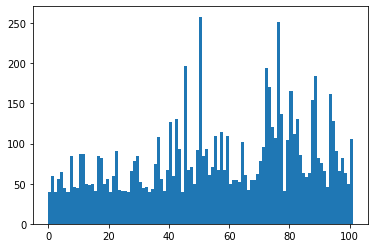
\includegraphics[width=0.6\textwidth]{dataset_hist.png}
    \caption{Histogram breakdown of the oxford flowers dataset, the X axis is the class label index.}
    \label{fig:dataset_hist}
\end{figure}

\clearpage

\section{Inception V3 Results Graphs}

\subsection{Full HP Results}

\label{subsec:hp}

\begin{figure}[h]\
    \centering
    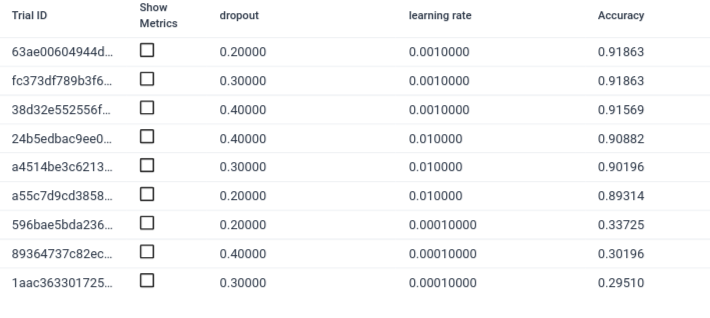
\includegraphics[width=\textwidth]{full_hp.png}
    \caption{Table of full HP training results as seen in TensorBoard.}
    \label{fig:hp_full}
\end{figure}

\subsection{Loss}

\label{subsec:loss}

\begin{figure}[h]\
    \centering
    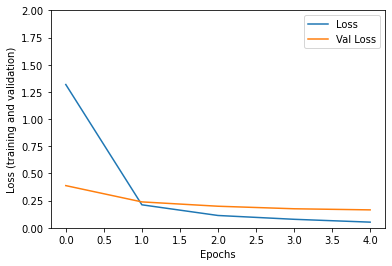
\includegraphics[width=0.6\textwidth]{Loss.png}
    \caption{Graph of loss against the number of training steps.}
    \label{fig:incep_loss}
\end{figure}

\clearpage

\section{Requirements}

Sources:
\begin{itemize}
    \item SS: Saahil Shihaz
    \item AD: Android Developers
    \item TF: TensorFlow
    \item MY: Material You
\end{itemize}

Priorities:
\begin{itemize}
    \item H: High
    \item M: Medium
    \item L: Low
\end{itemize}

\subsection{Functional Requirements}
\label{subsec:funcreq}

\begin{table}[h!]
    \begin{tabularx}{ \textwidth }{ 
        | >{\raggedright\arraybackslash}X 
        | >{\raggedright\arraybackslash}X 
        | >{\raggedright\arraybackslash}X
        | >{\raggedright\arraybackslash}X| }
        \hline
        No. & Description & Source & Priority \\
        \hline
        1 & 
        The app must run on an Android device.
        & SS & H \\
        \hline
        2 & 
        The app must be able to capture an image.
        & SS, AD & H \\
        \hline
        2.1 & 
        The app must be able to display a captured image. 
        & SS, AD & H \\
        \hline
        3 &
        The app must use the Inception V3 model trained in chapter 3 to process captured images. 
        & SS, TF & H \\
        \hline
        4 &
        The app must display the guesses produced by the model within 500 milliseconds.
        & SS & H \\
        \hline
        4.1 &
        The app must show the top three guesses as well as their individual percentage probabilities ranked from highest
        to lowest.
        & SS & H \\
        \hline
        4.2 &
        The app should show a small preview of the flowers next to the guesses.
        & SS & M \\
        \hline
        5 & 
        The app must display the time it takes to process an image in milliseconds.
        & SS & H \\
        \hline
        6 &
        The app could contain additional pages that provide more pictures and information about the flower that can be 
        accessed by clicking on the flower's icon.
        & SS & L \\
        \hline
    \end{tabularx}
    \label{table:func}
\end{table}
\clearpage
\subsection{Non-functional Requirements}
\label{subsec:nonreq}

\begin{table}[h!]
    \begin{tabular}{ |l|l|l|l| }
        \hline
        No. & Description & Source & Priority \\
        \hline
        1 & 
        The app must function with minimal bugs. 
        & SS & H \\
        \hline
        2 & 
        The app must follow the Material You design specifications.
        & MY & L \\
        \hline
    \end{tabular}
    \label{table:nonfunc}
\end{table}

\subsection{SDK percentage}

\label{subsec:sdk}

\begin{figure}[h]\
    \centering
    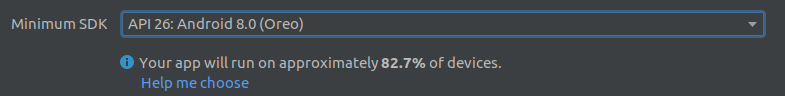
\includegraphics[width=\textwidth]{Min_SDK.png}
    \caption{The percentage of devices that API level 8 will run according to Android Studio.}
    \label{fig:sdk}
\end{figure}

\clearpage

\subsection{Model performance list}

\label{subsec:models}

\begin{figure}[h]\
    \centering
    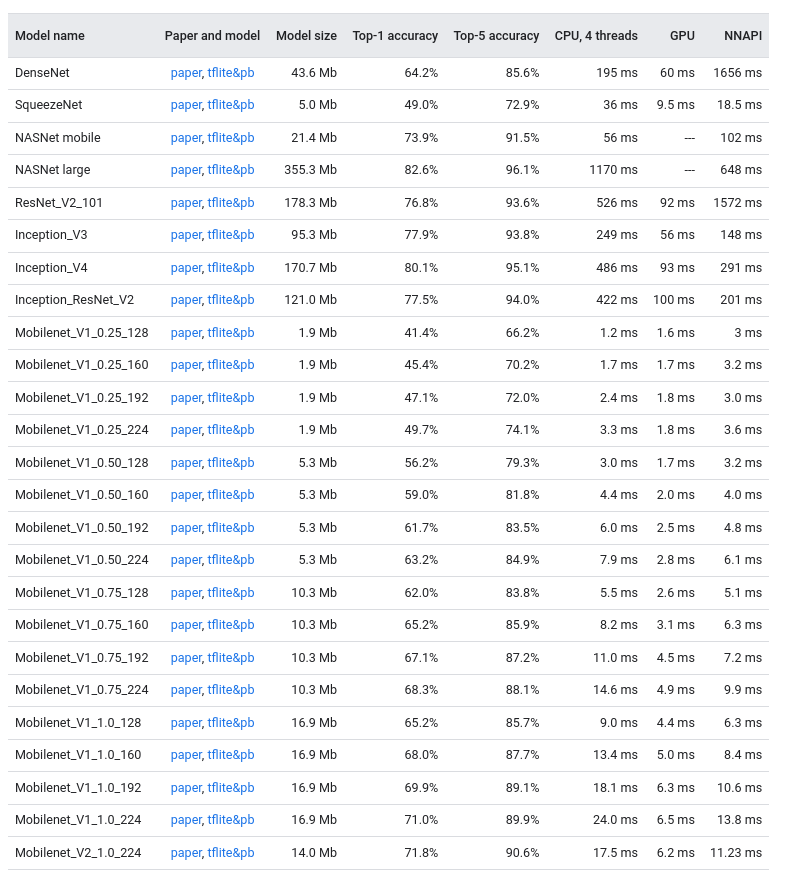
\includegraphics[width=\textwidth]{models.png}
    \caption{The list of models and their performance metrics on the TensorFlow site \citep{TFhostedmodels}.}
    \label{fig:models}
\end{figure}
\clearpage

\section{Design}

\subsection{Prototype}

\begin{figure}[h]\
    \centering
    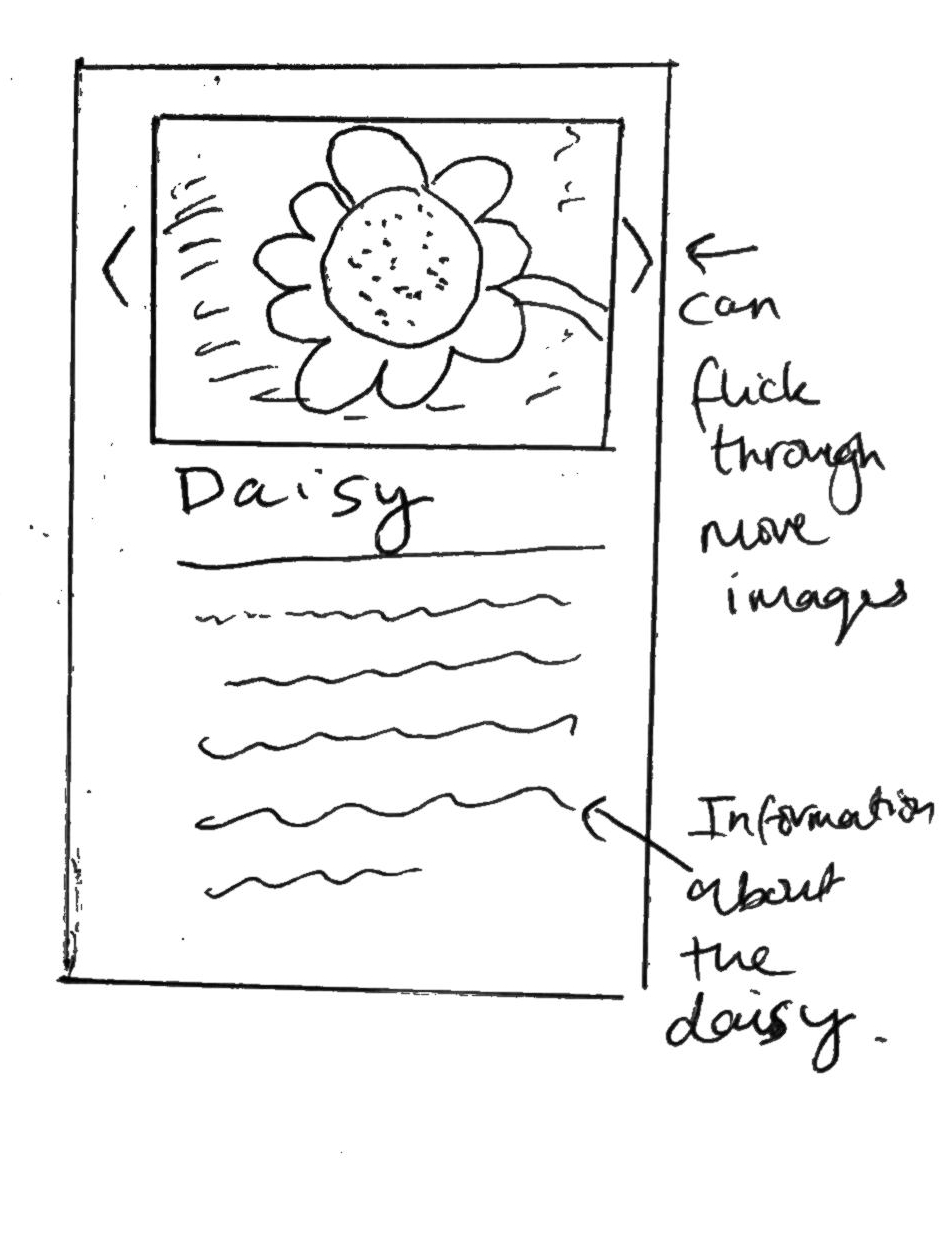
\includegraphics[width=0.6\textwidth]{Info_Sketch.jpg}
    \caption{Sketch of the flower information page}
    \label{fig:sketch_info}
\end{figure}

\section{Testing}
\subsection{Testing device specifications}

\label{subsec:phone_spec}

Samsung Galaxy S20 5G

\par

Apr 27, 2022 5:57

\par

Hardware \\
exynos990 \\
Cores: 8 \\
CPU: \\
2 x M5 \\
2 x Cortex-A76 \\
4 x Cortex-A55 \\
Process: 7 nm LPP \\
Frequencies: \\
442 MHz - 2002 MHz \\
507 MHz - 2504 MHz \\ 
546 MHz - 2730 MHz

\par

GRAPHICS \\
Vendor: ARM \\
GPU: Mali-G77 \\
OpenGL: OpenGL ES 3.2 \\
Max frequency: 800 MHz \\
Resolution: 2400 x 1080 \\
Screen density: 424.48477 ppi \\
Screen size (estimated): 6.2 in / 158 mm

\par

RAM \\
RAM size: 12 GB \\
Type: LPDDR5 2750 MHz \\
Bandwidth: 44 GB/s \\
Channels: 16-bit quad channel

\par

Storage \\
Size: 128 GB \\
Filesystem: sdcardfs \\

\par

DEVICE \\
Model: SM-G981B \\
Codename: x1s \\
Manufacturer: samsung \\
Manufacturing date: October 5, 2020

\par

System \\
Android Version: Android 12 \\
Build: SP1A.210812.016.G981BXXSDFVC9 \\
ROM base: G981BXXSDFVC9 \\
Security patch: April 1, 2022 \\
Architecture: aarch64 (64-bit) \\
Instruction sets: arm64-v8a armeabi-v7a armeabi \\
Kernel: Linux version 4.19.87-23725627 (dpi@21DJ7D03) (Android (dev based on r349610)
clang version 8.0.8 (based on LLVM 8.0.8svn))

\par

Battery \\
Technology: Li-ion \\
Health: Good \\
Capacity (reported by system): 3880 mAh

\par

CAMERA \\
Resolution: 12.2 MP (4032x3024) \\
Focal length: 2.2 mm \\
35mm equivalent focal length: 13.5 mm \\
Sensor size: 5.64 x 4.23 mm \\ 
Crop factor: 6.1x \\
Field of view: 104.1 degrees \\
Pixel size: 1.40 micro metres \\
Aperture: 2.2 \\
Shutter speed: 1/11764 - 1/10 s \\
RAW mode: No \\
ISO sensitivity range: 50 - 3200 \\
RAW mode: Supported \\
Optical image stabilization: No \\
Front camera: 7.1 MP (3216x2208)

\subsection{Fine-tuning test}

\begin{figure}[h]\
    \centering
    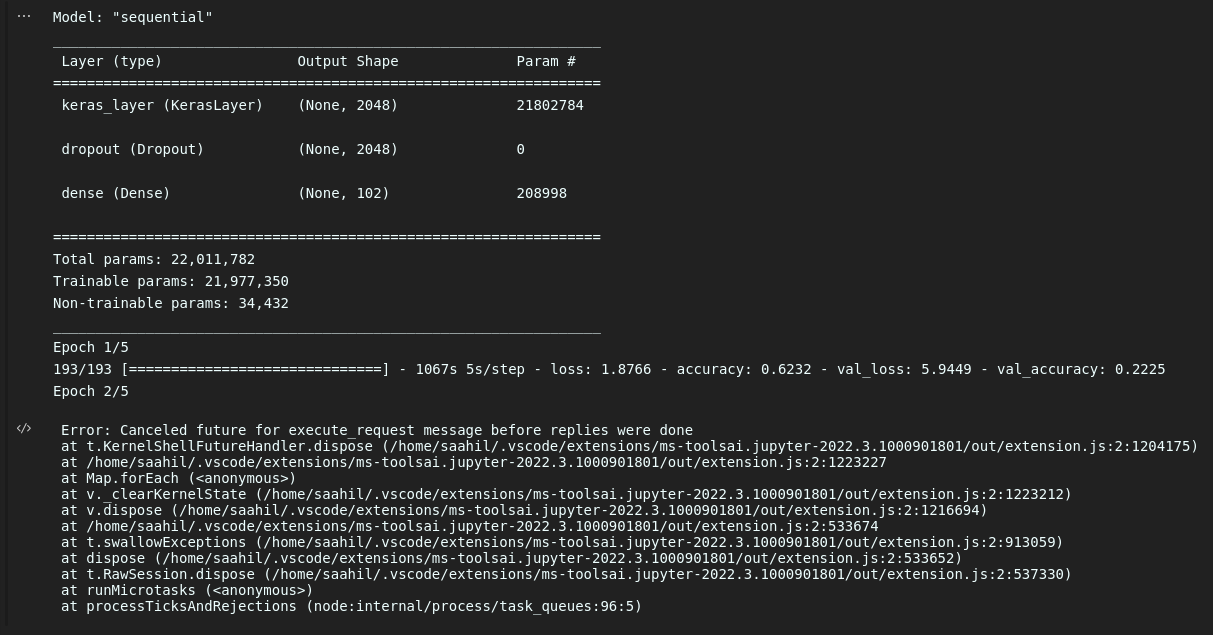
\includegraphics[width=\textwidth]{Error_Trainable.png}
    \caption{Error message due to the program being killed for using too much memory.}
    \label{fig:finetuning}
\end{figure}

\subsection{Results of functionality testing}
\label{subsec:functionality}

\begin{table}[h!]
    \begin{tabular}{ |l|l|l|l|l| }
        \hline
        Figure & Prediction & Prob. (\%) & Actual & Time (ms) \\
        \hline
        \ref{fig:anthurium} & Anthurium & 78 & Anthurium & 351 \\
        \hline
        \ref{fig:columbine} & Columbine & 48 & Unknown & 376 \\
        \hline
        \ref{fig:cyclamen} & Cyclamen & 47 & Orchid & 364 \\
        \hline
        \ref{fig:daffodil} & Daffodil & 93 & Daffodil & 378 \\
        \hline
        \ref{fig:daisy} & Oxeye Daisy & 96 & Oxeye Daisy & 379 \\
        \hline
        \ref{fig:dandelion} & Dandelion & 100 & Dandelion & 393 \\
        \hline
        \ref{fig:dandelion_2} & Dandelion & 88 & Dandelion & 373 \\
        \hline
        \ref{fig:rose} & Rose & 97 & Rose & 316 \\
        \hline
    \end{tabular}
    \caption{Table of predictions for 8 different flowers found in the vicinity.}
    \label{table:results}
\end{table}

\clearpage

\begin{figure}[h]\
    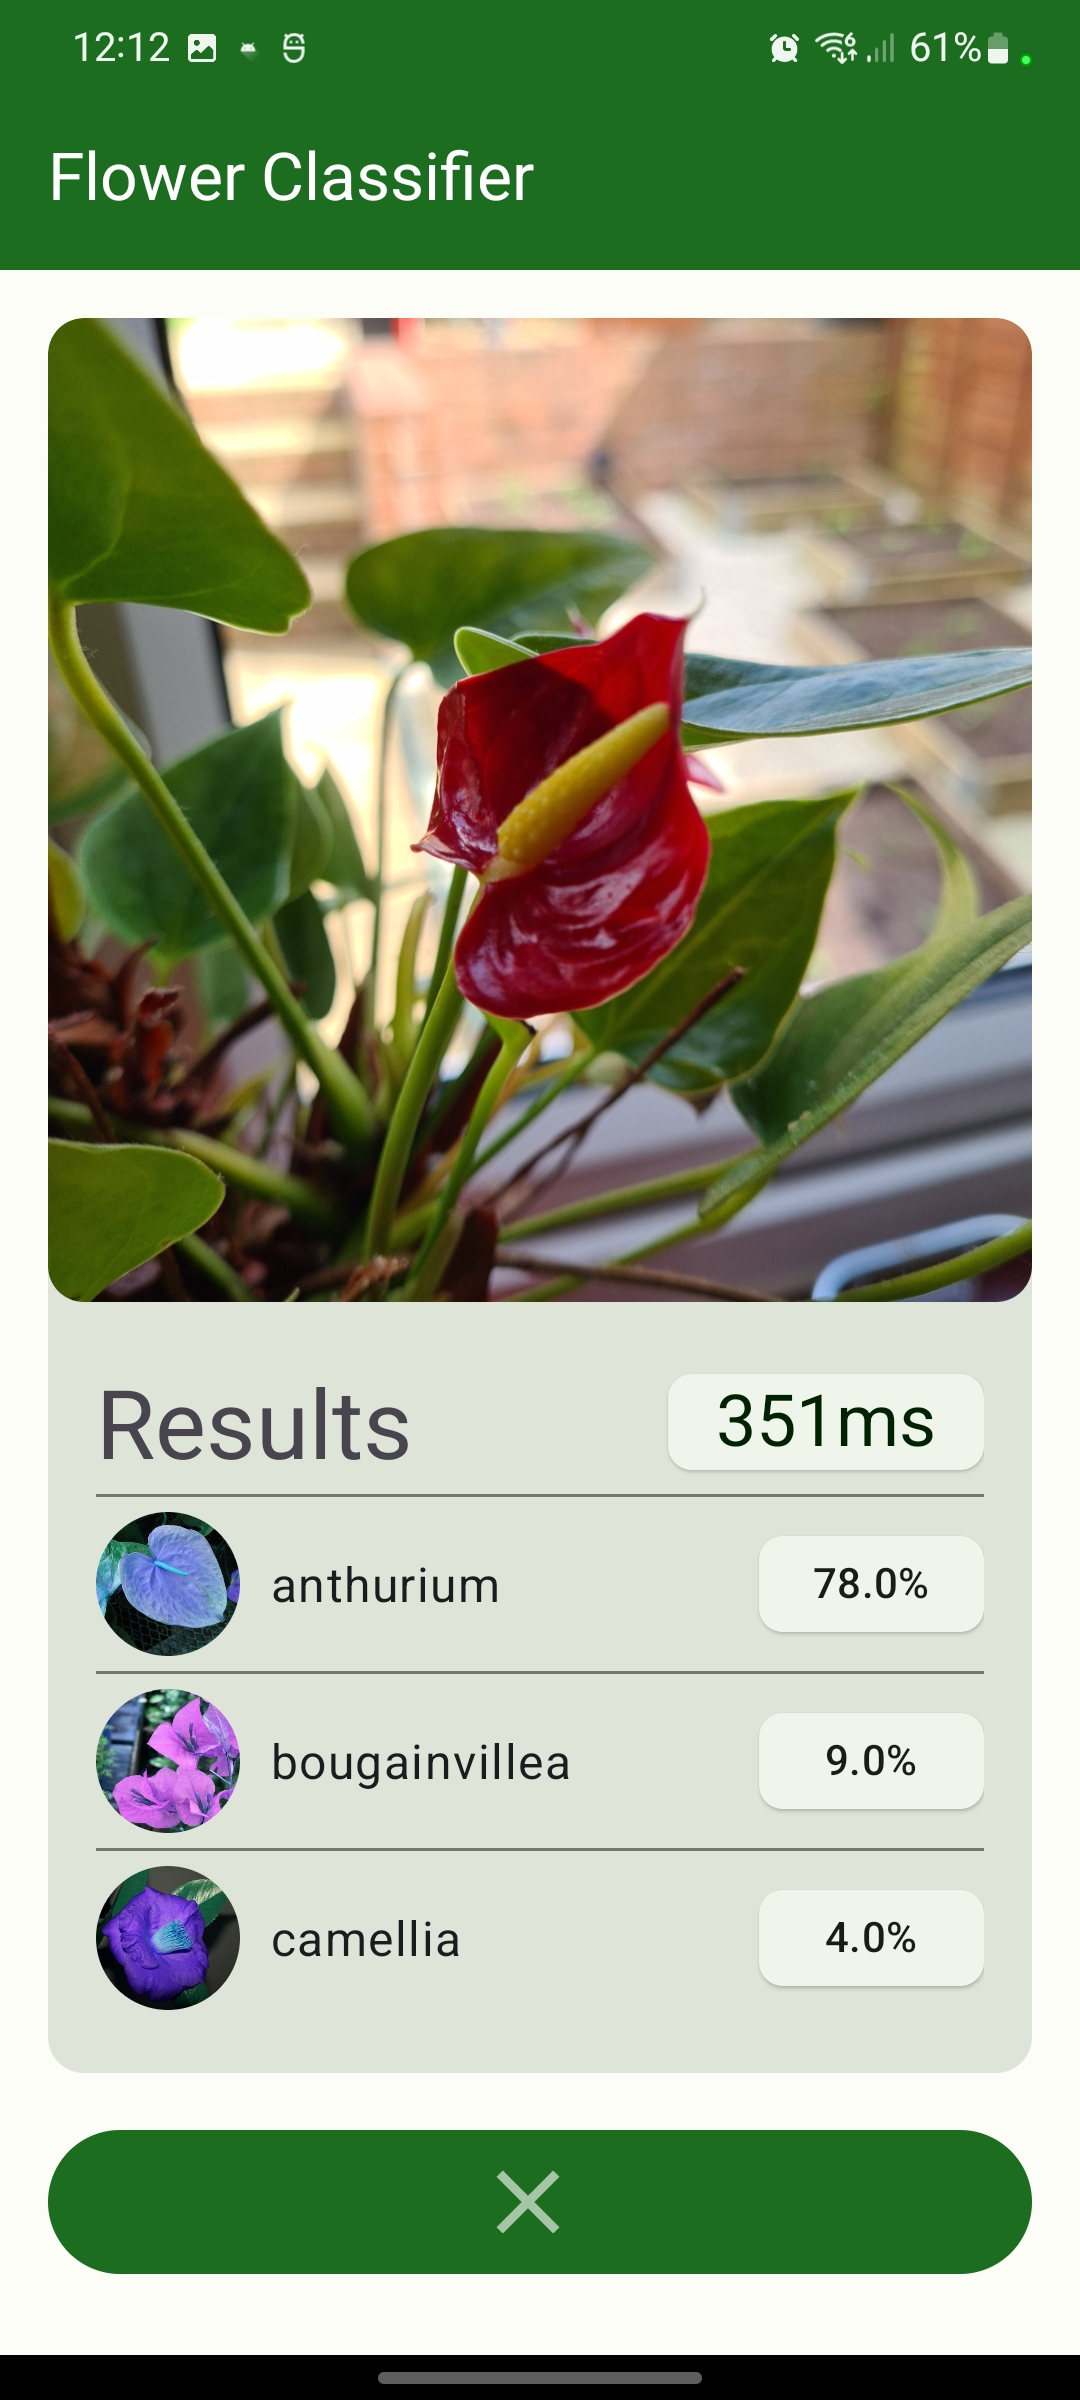
\includegraphics[width=0.3\textwidth]{anthurium.jpg}
    \caption{Classifying an Anthurium using the app.}
    \label{fig:anthurium}
\end{figure}

\begin{figure}[h]\
    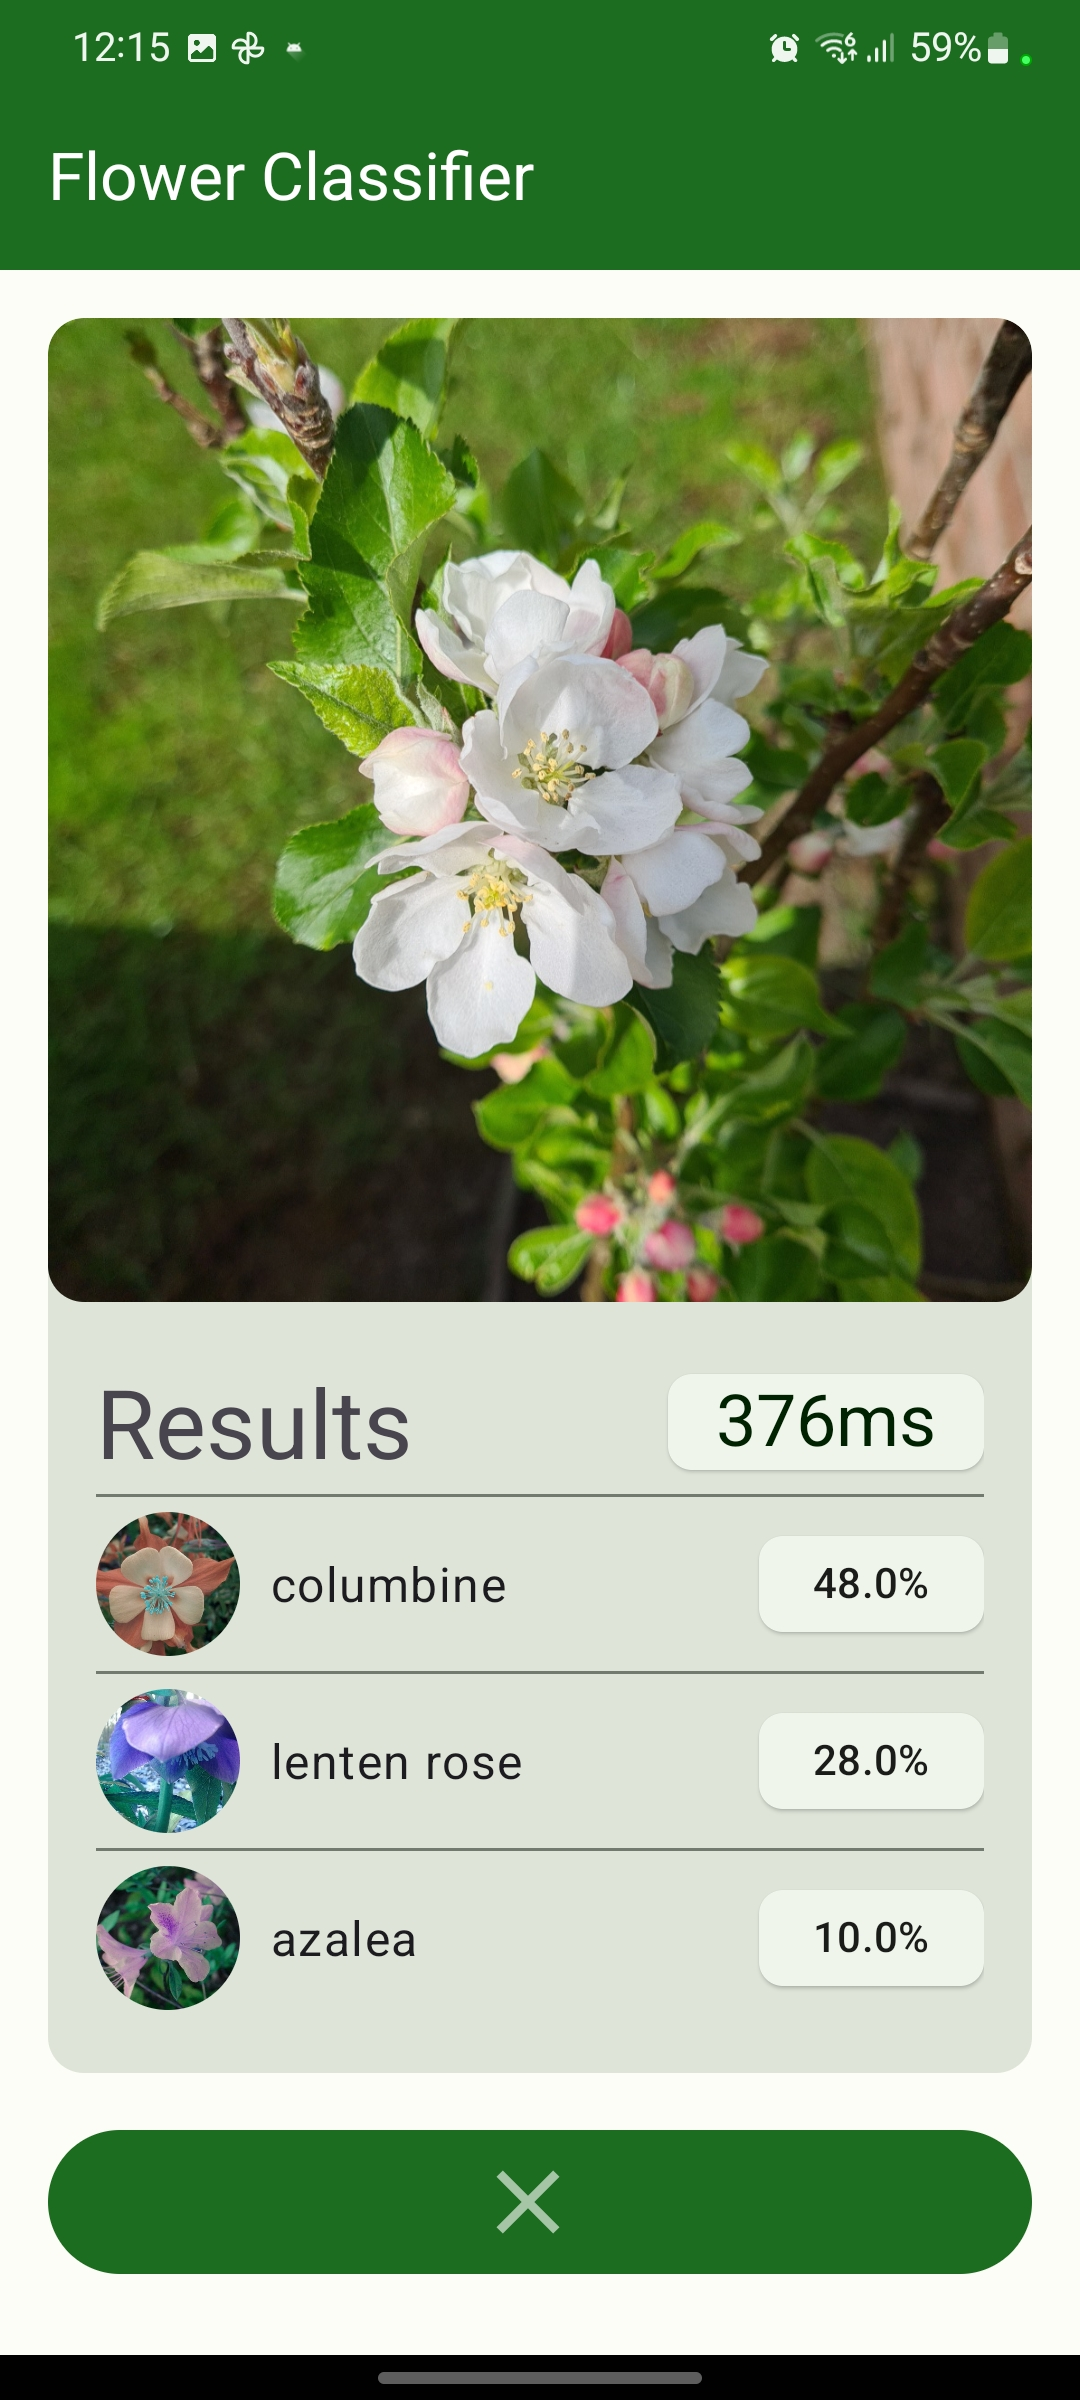
\includegraphics[width=0.3\textwidth]{columbine.jpg}
    \caption{Classifying a Columbine using the app.}
    \label{fig:columbine}
\end{figure}


\begin{figure}[h]\
    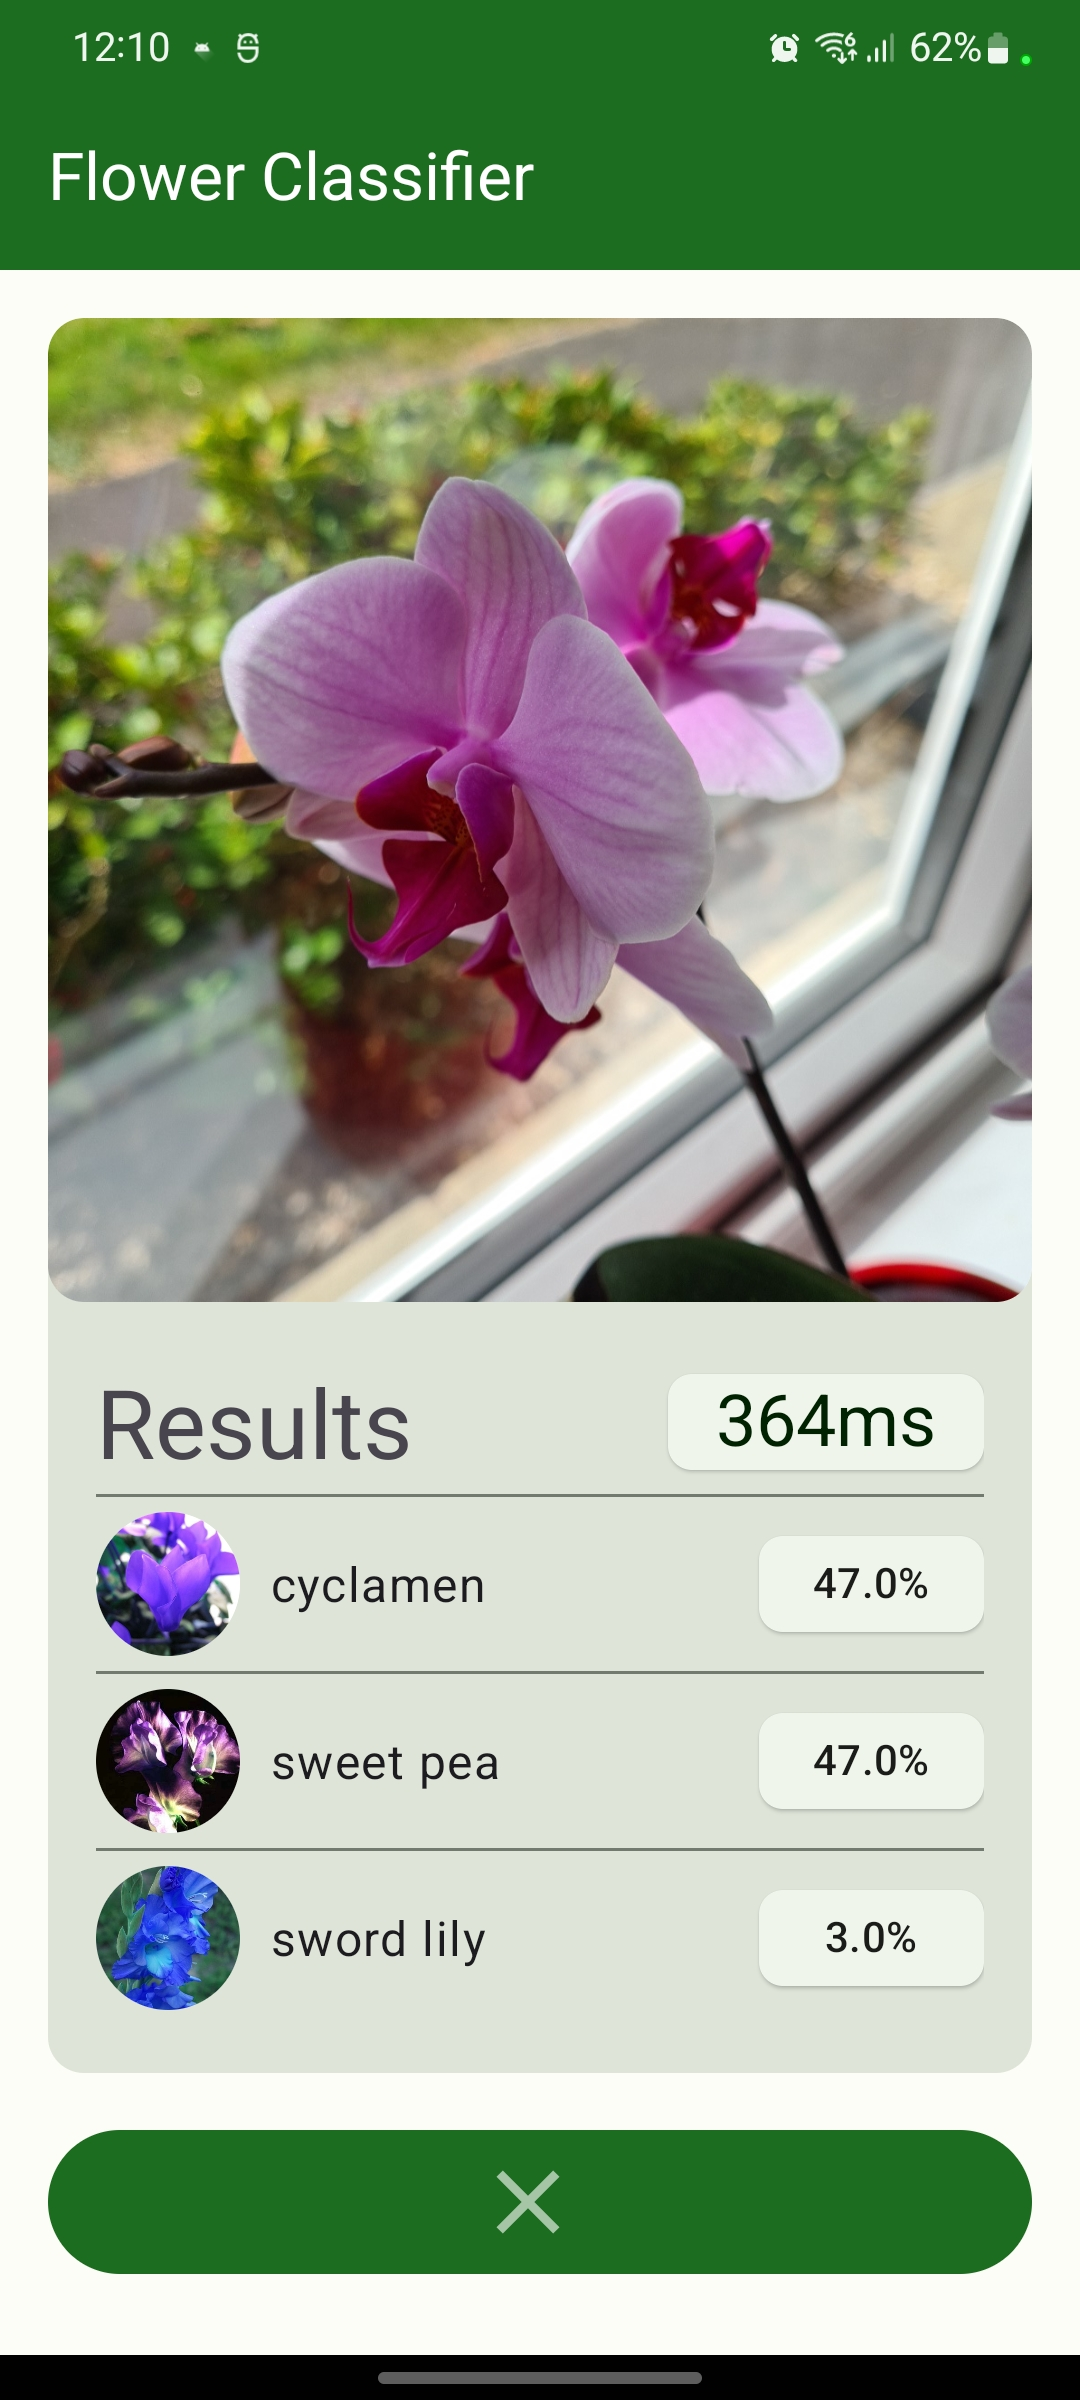
\includegraphics[width=0.3\textwidth]{cyclamen.jpg}
    \caption{Classifying an Orchid using the app.}
    \label{fig:cyclamen}
\end{figure}

\begin{figure}[h]\
    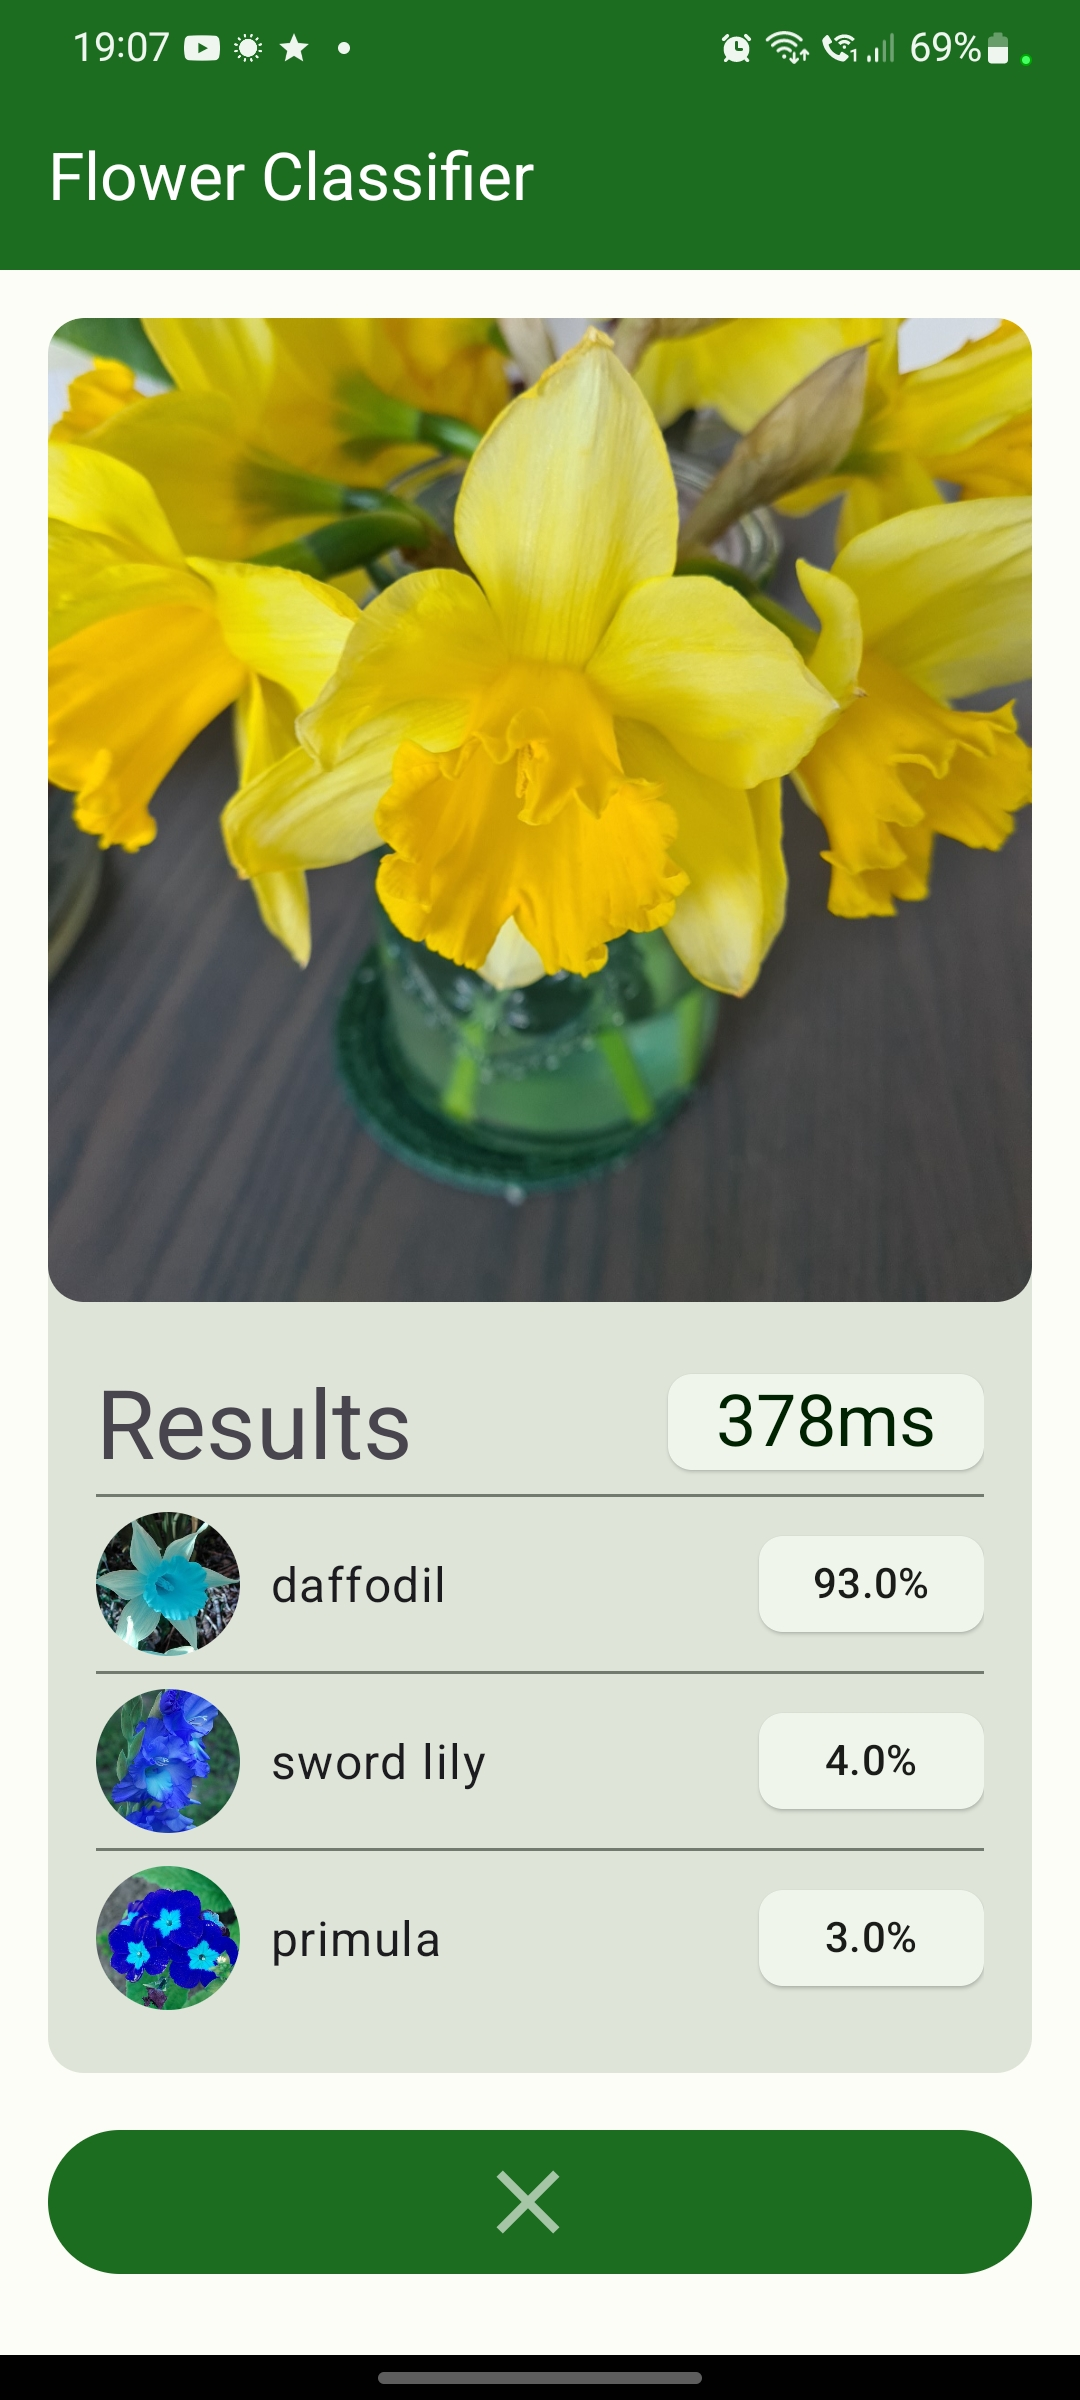
\includegraphics[width=0.3\textwidth]{daffodil.jpg}
    \caption{Classifying a Daffodil using the app.}
    \label{fig:daffodil}
\end{figure}

\begin{figure}[h]\
    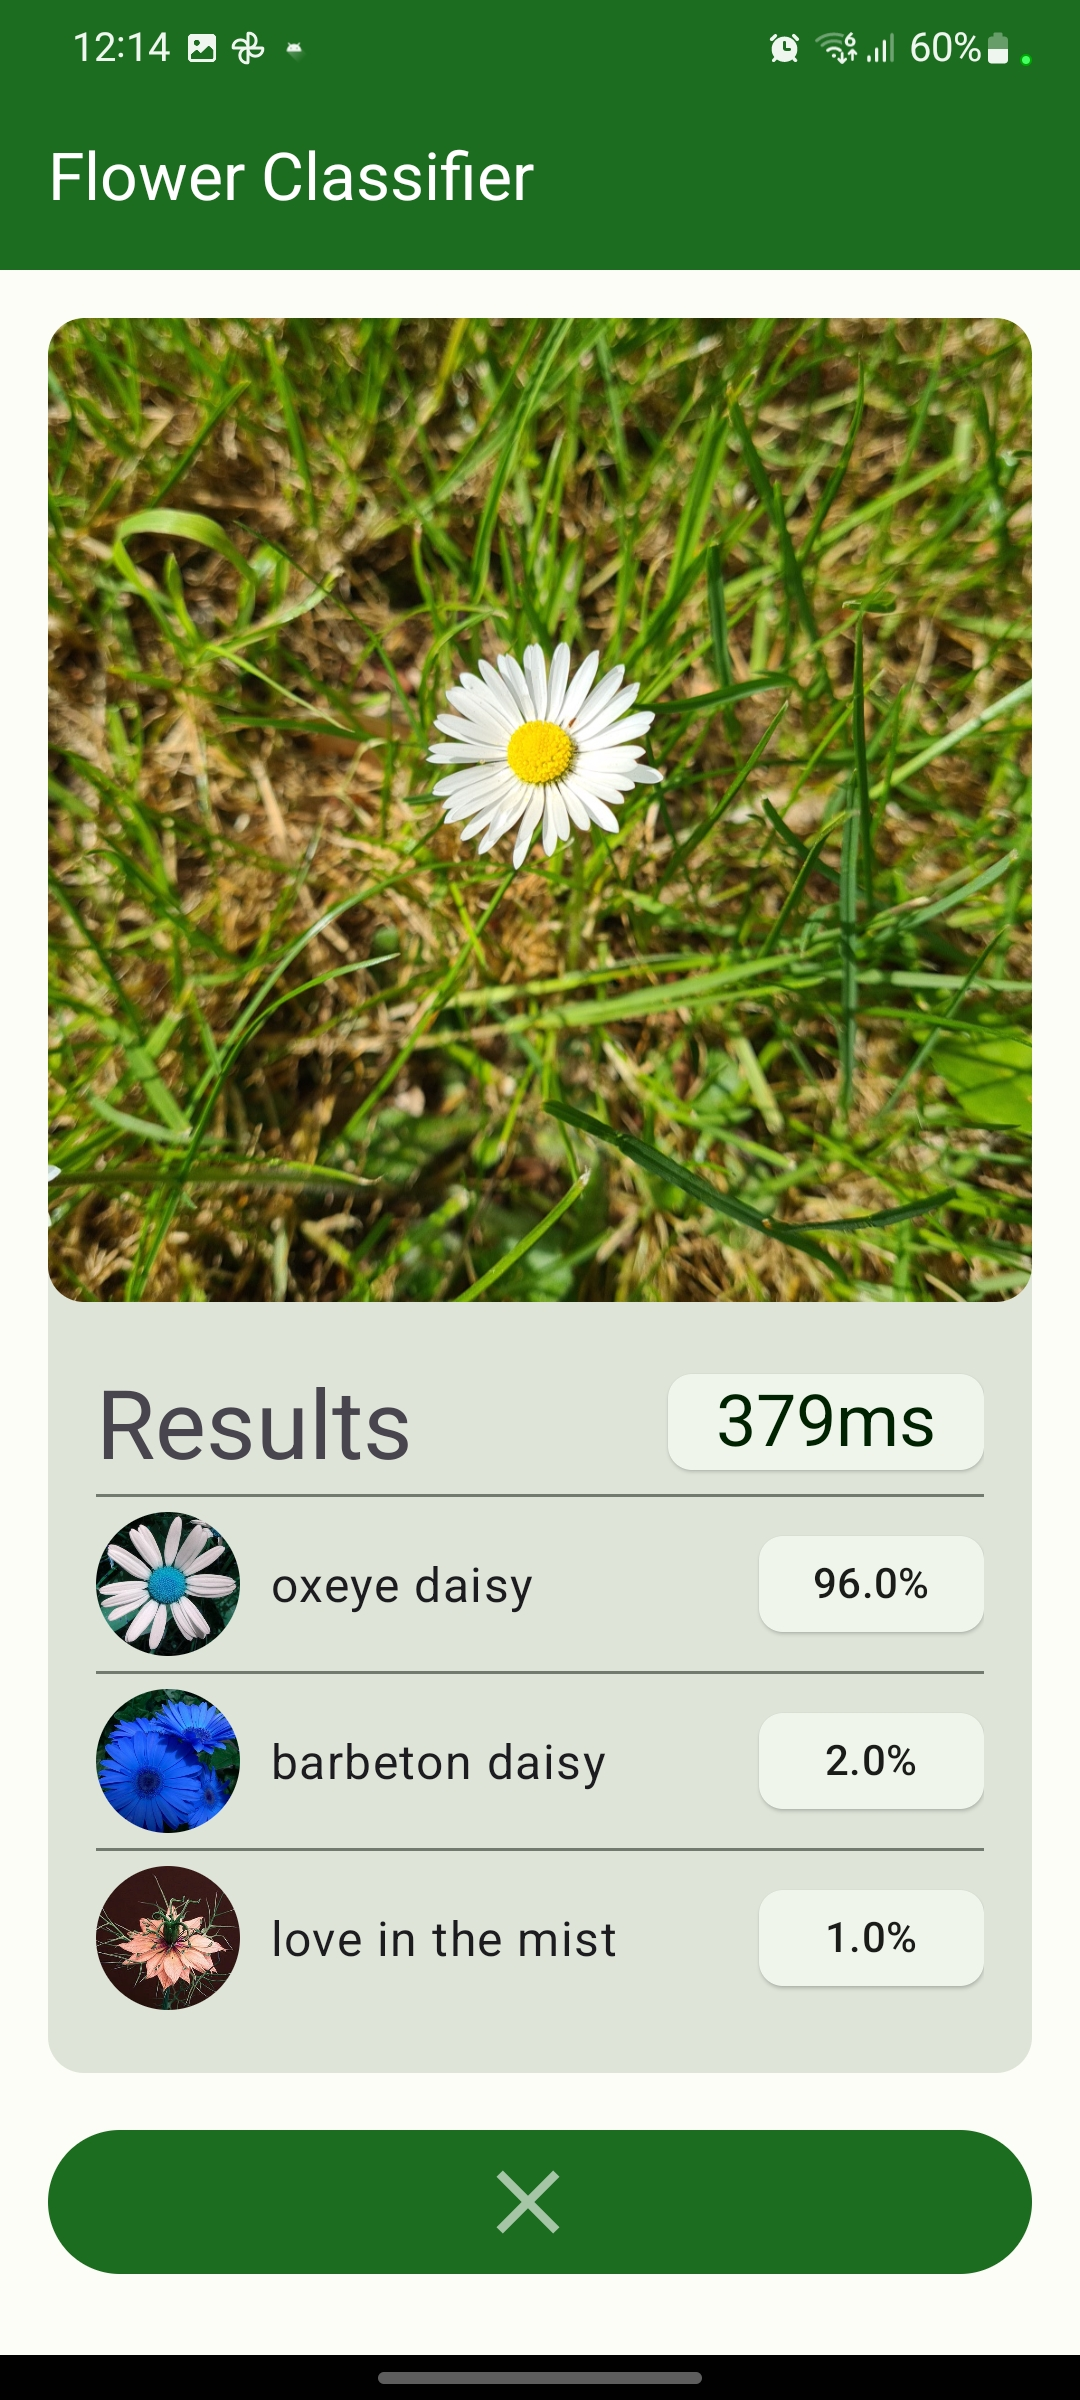
\includegraphics[width=0.3\textwidth]{daisy.jpg}
    \caption{Classifying a Daisy using the app.}
    \label{fig:daisy}
\end{figure}

\begin{figure}[h]\
    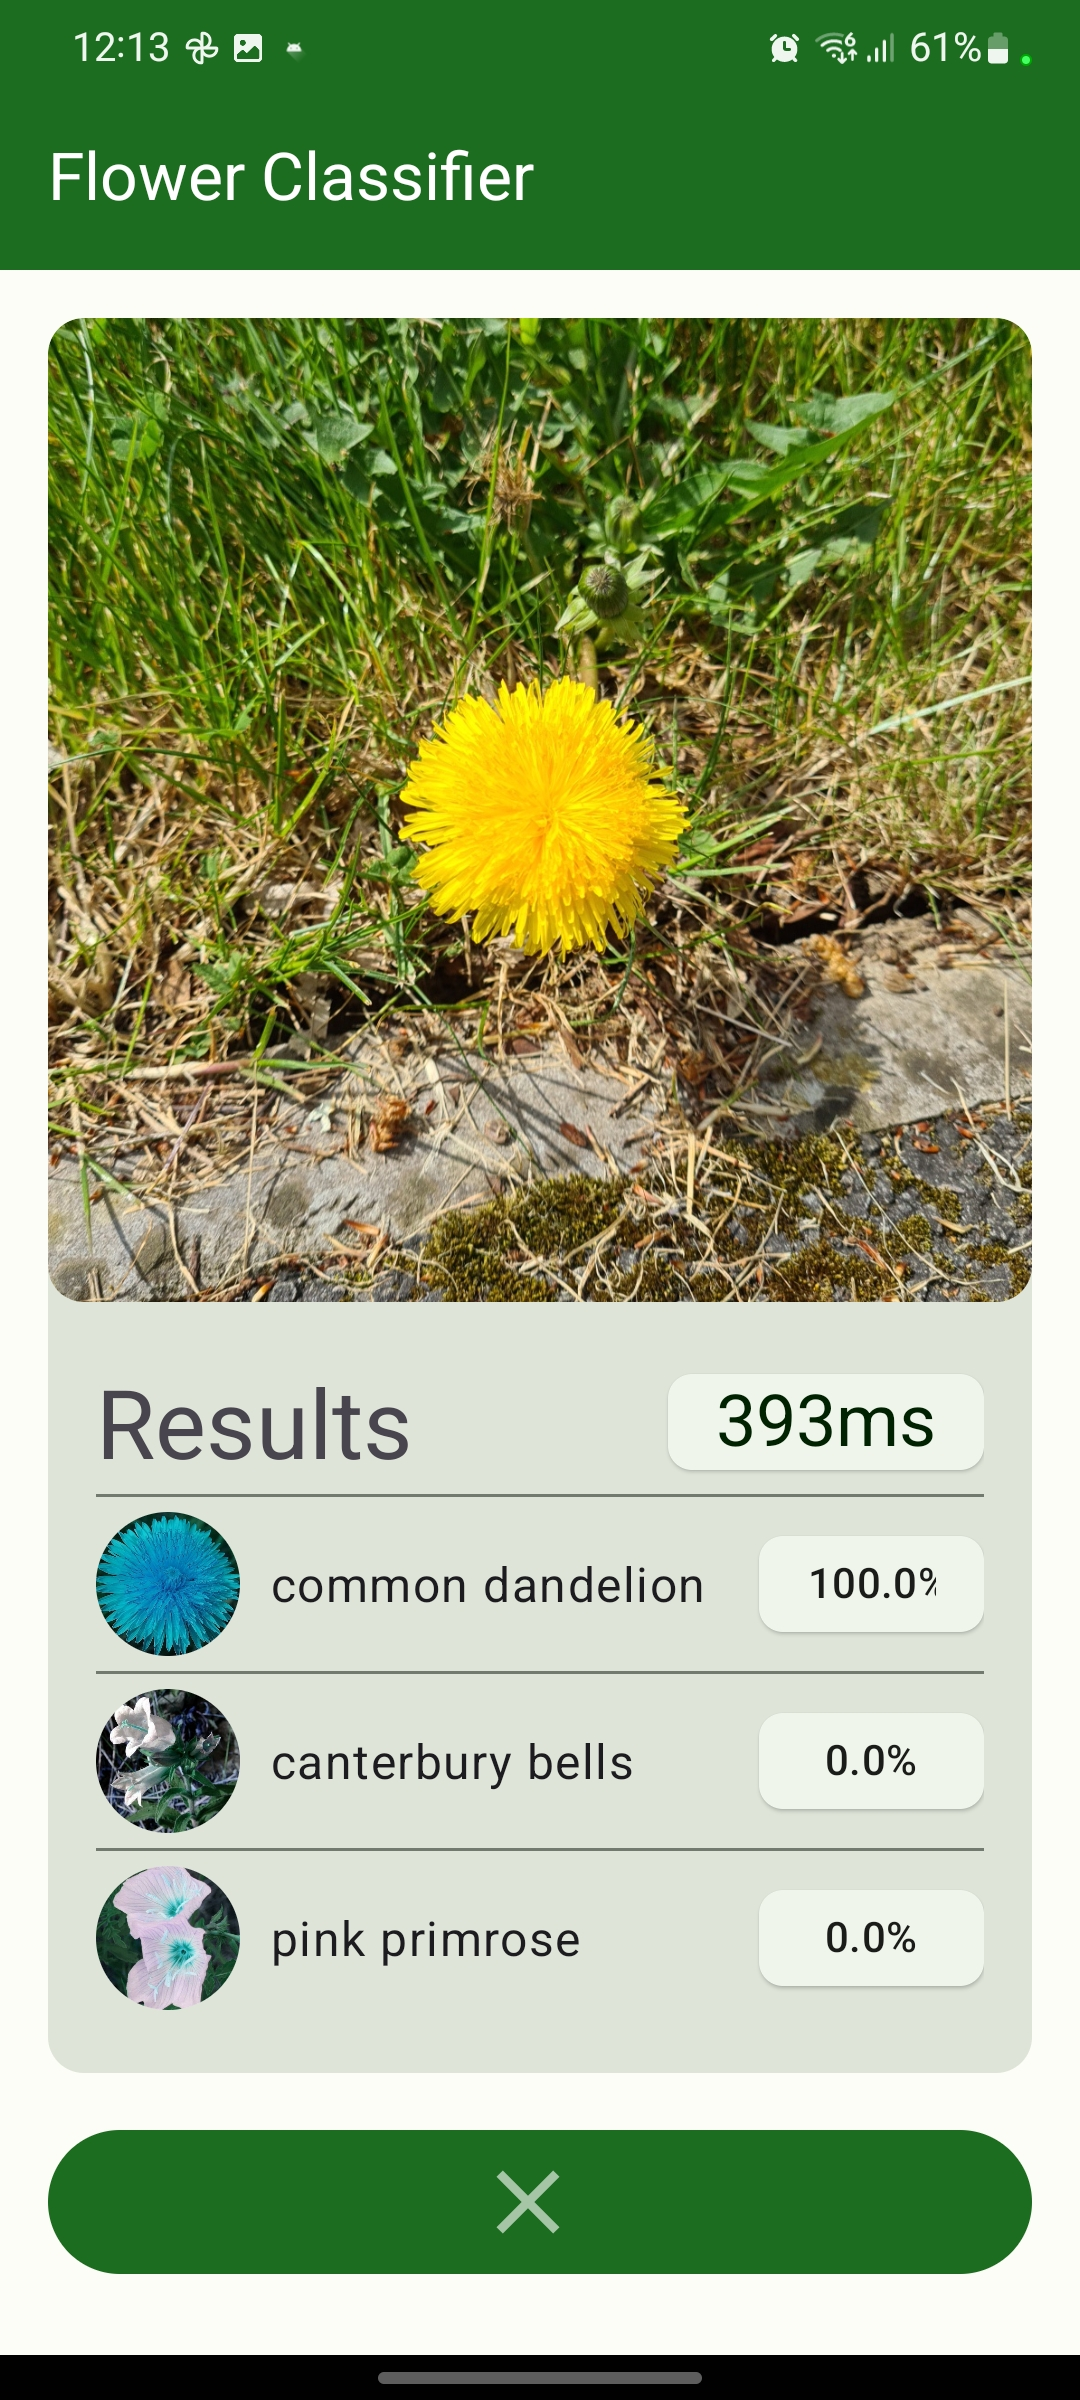
\includegraphics[width=0.3\textwidth]{dandelion.jpg}
    \caption{Classifying a yellow Dandelion using the app.}
    \label{fig:dandelion}
\end{figure}

\begin{figure}[h]\
    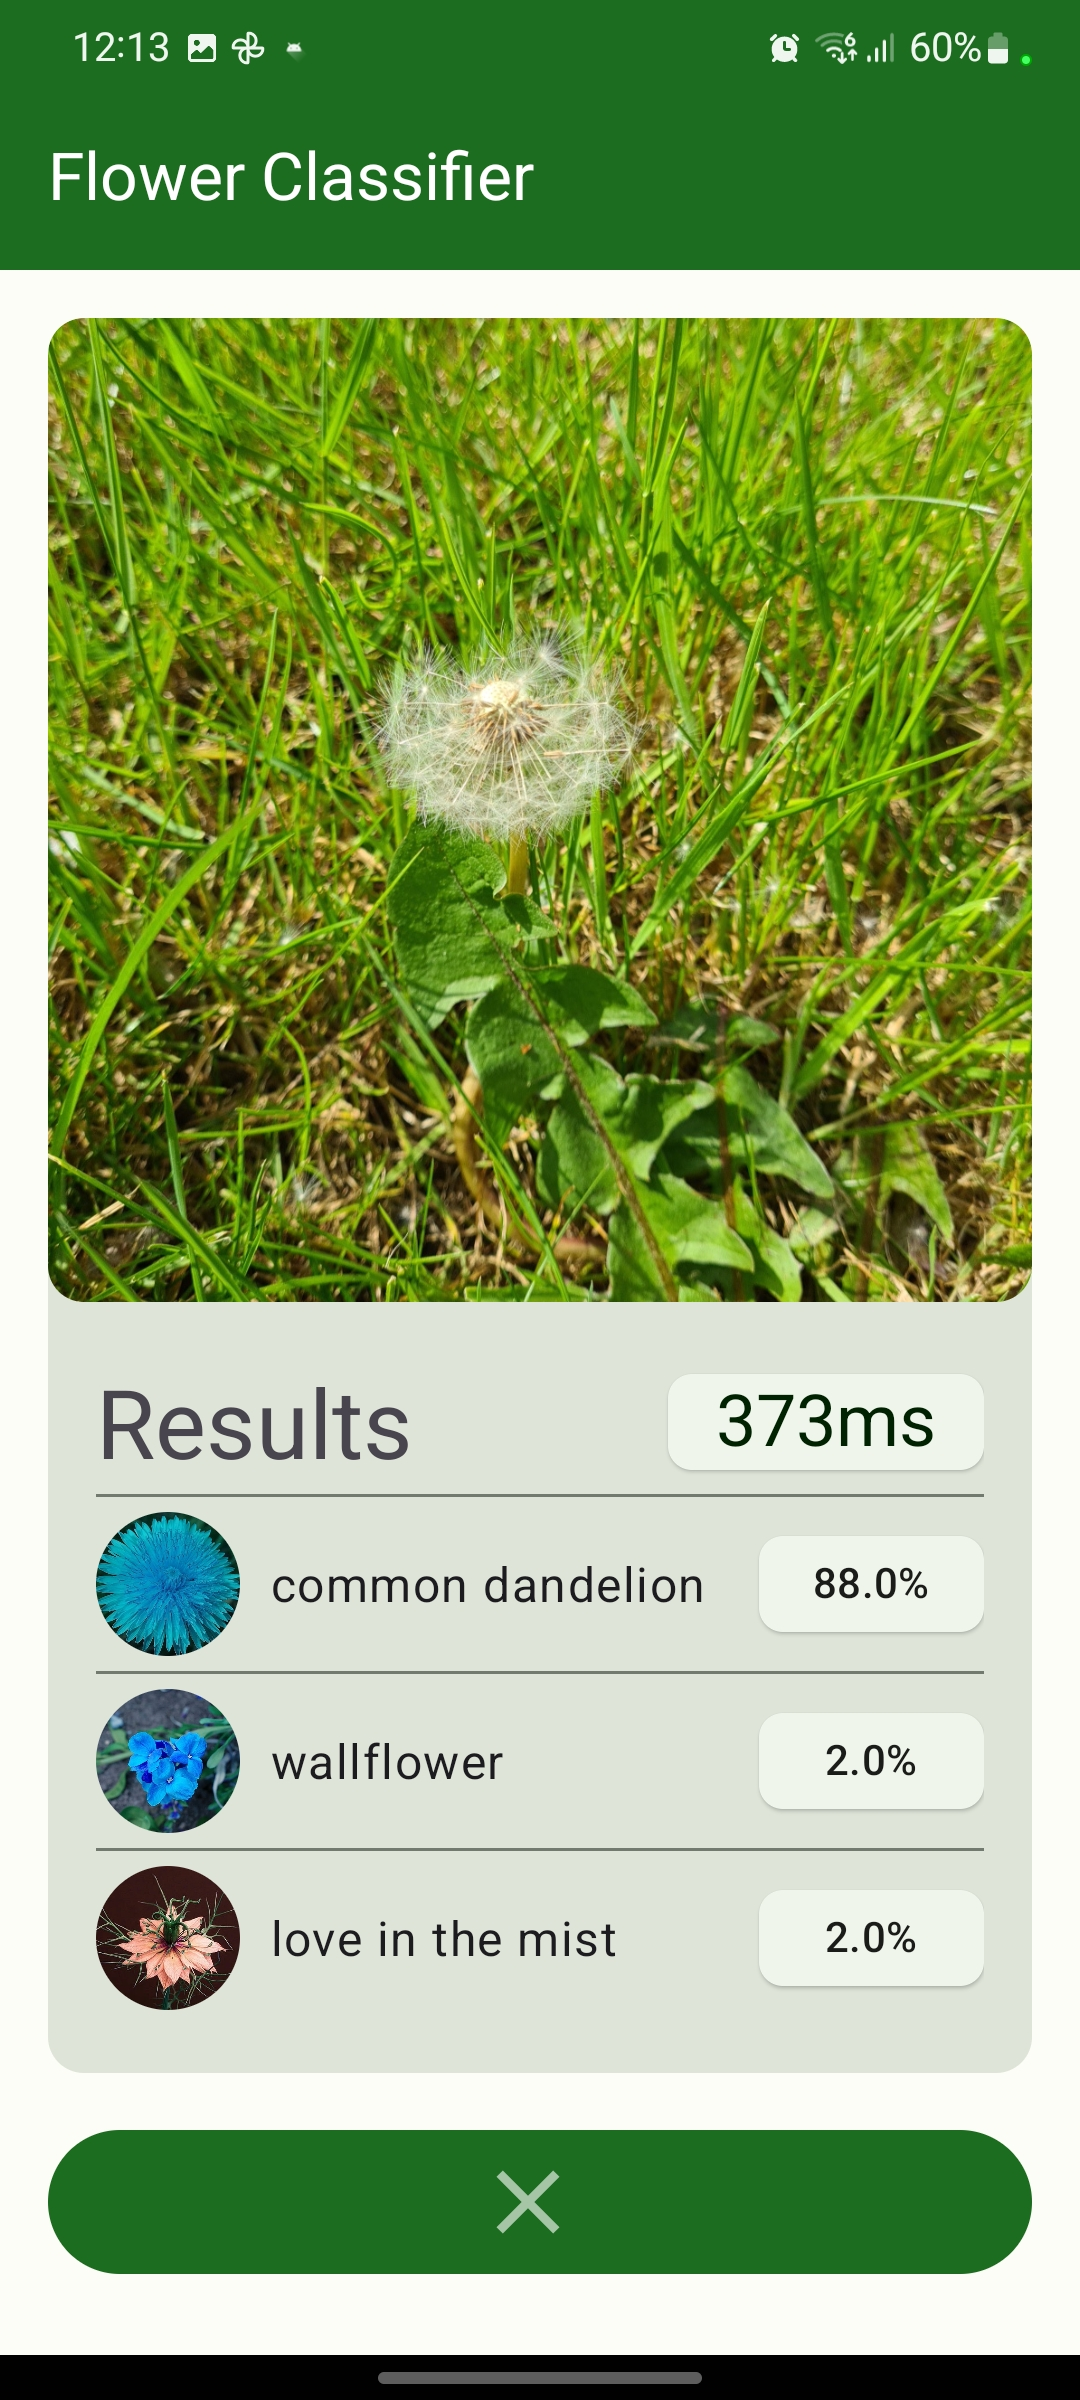
\includegraphics[width=0.3\textwidth]{dandelion_2.jpg}
    \caption{Classifying a white Dandelion using the app.}
    \label{fig:dandelion_2}
\end{figure}


\begin{figure}[h]\
    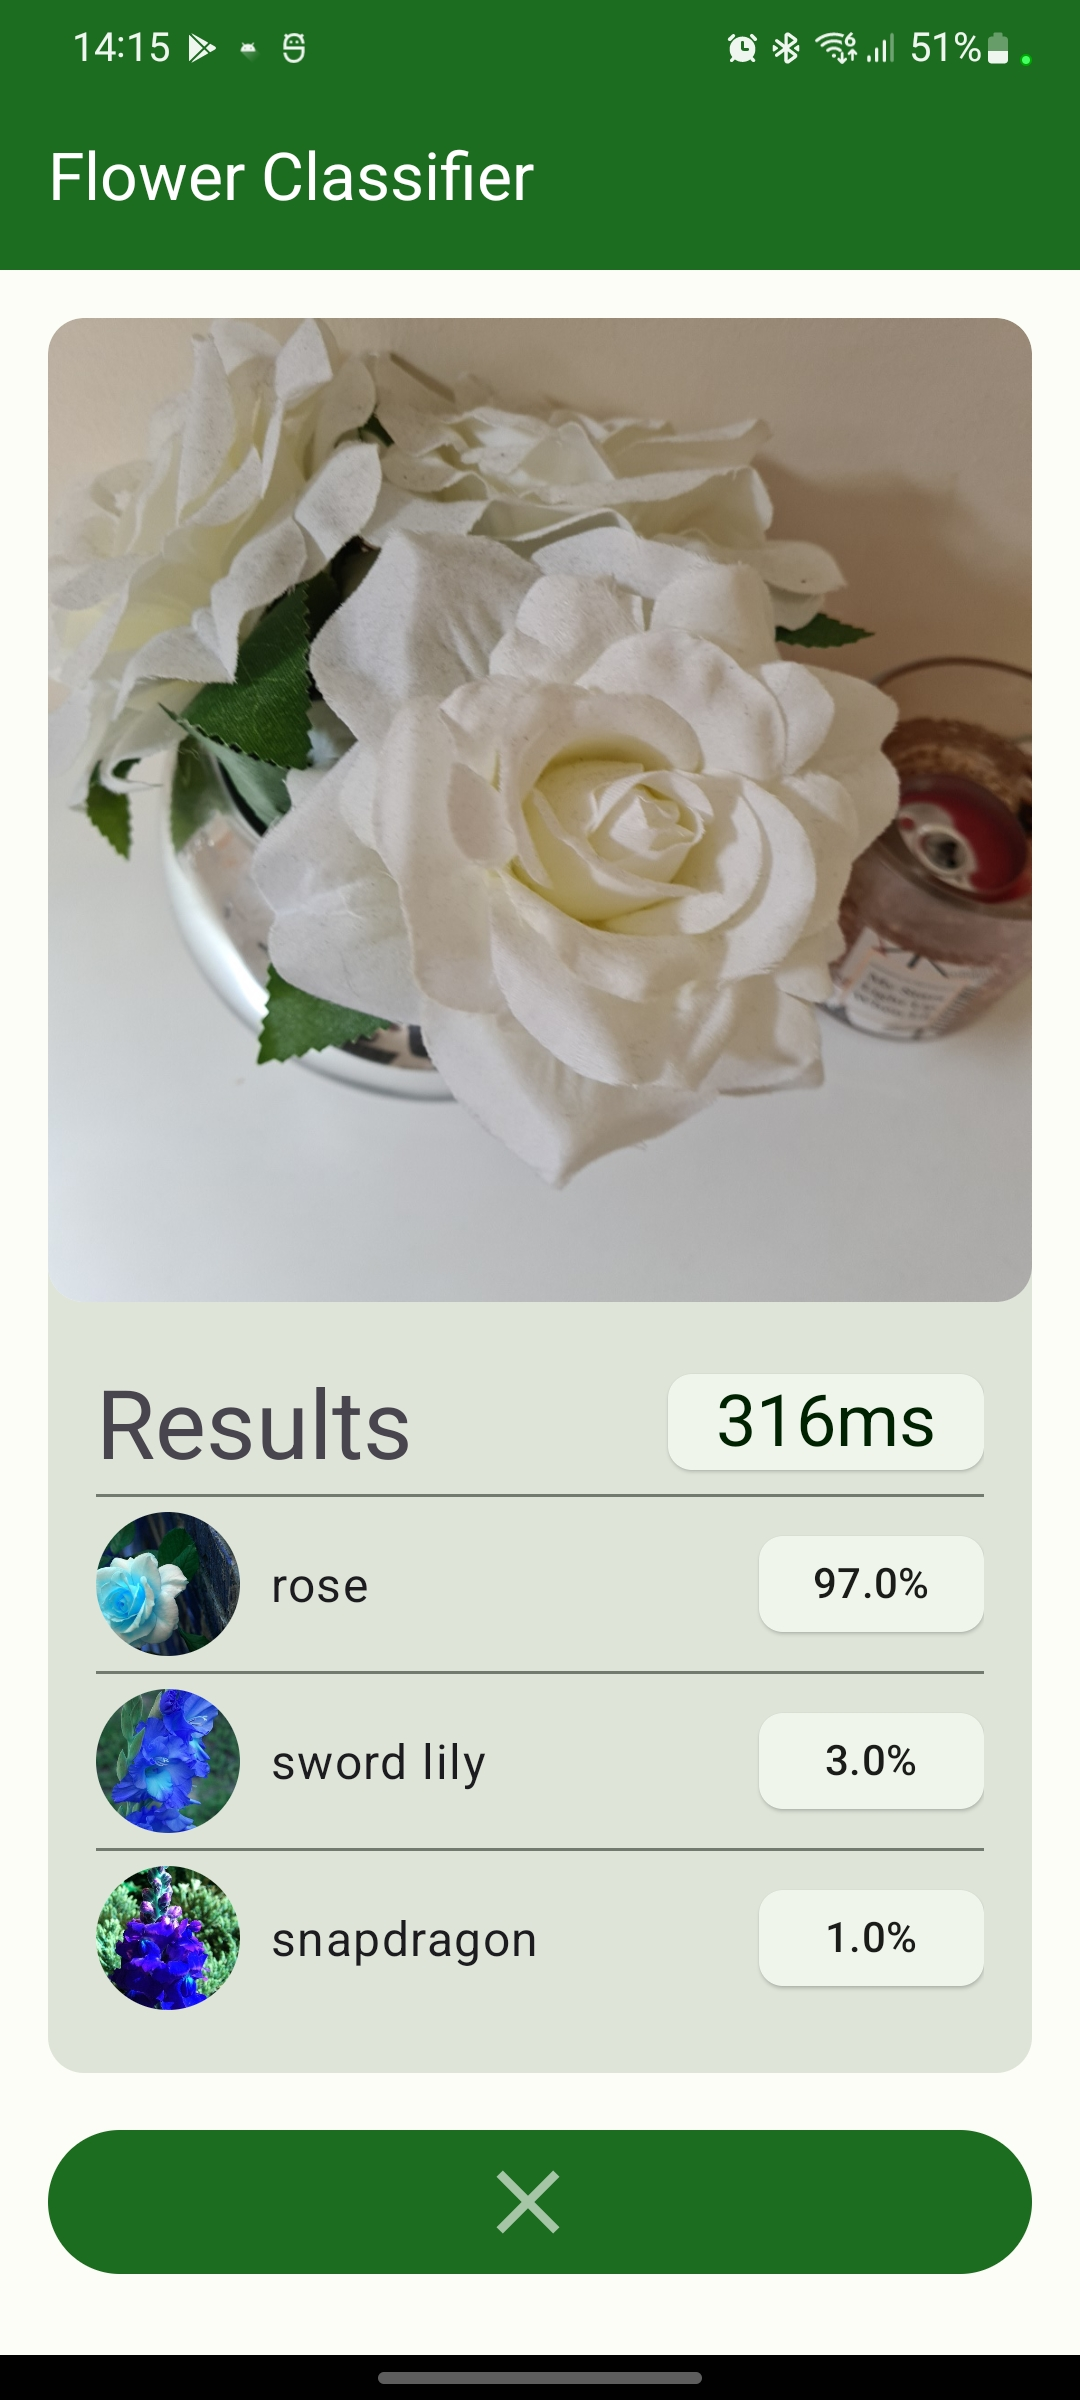
\includegraphics[width=0.3\textwidth]{rose.jpg}
    \caption{Classifying a Rose using the app.}
    \label{fig:rose}
\end{figure}

\clearpage


\subsection{Results of distance testing}
\label{subsec:distance}

\begin{table}[h!]
    \begin{tabular}{ |l|l|l|l| }
        \hline
        Figure & Distance (cm) & Prediction & Prob. (\%)\\
        \hline
        \ref{fig:rose_4} & 4 & Rose & 39 \\
        \hline
        \ref{fig:rose_15} & 15 & Rose & 78 \\
        \hline
        \ref{fig:rose_35} & 35 & Sword Lily & 56 \\
        \hline
        \ref{fig:rose_60} & 60 & Carnation & 72 \\ 
        \hline
    \end{tabular}
    \caption{Results from attempting to identify a rose at different distances.}
    \label{table:distance}
\end{table}

\begin{figure}[h]\
    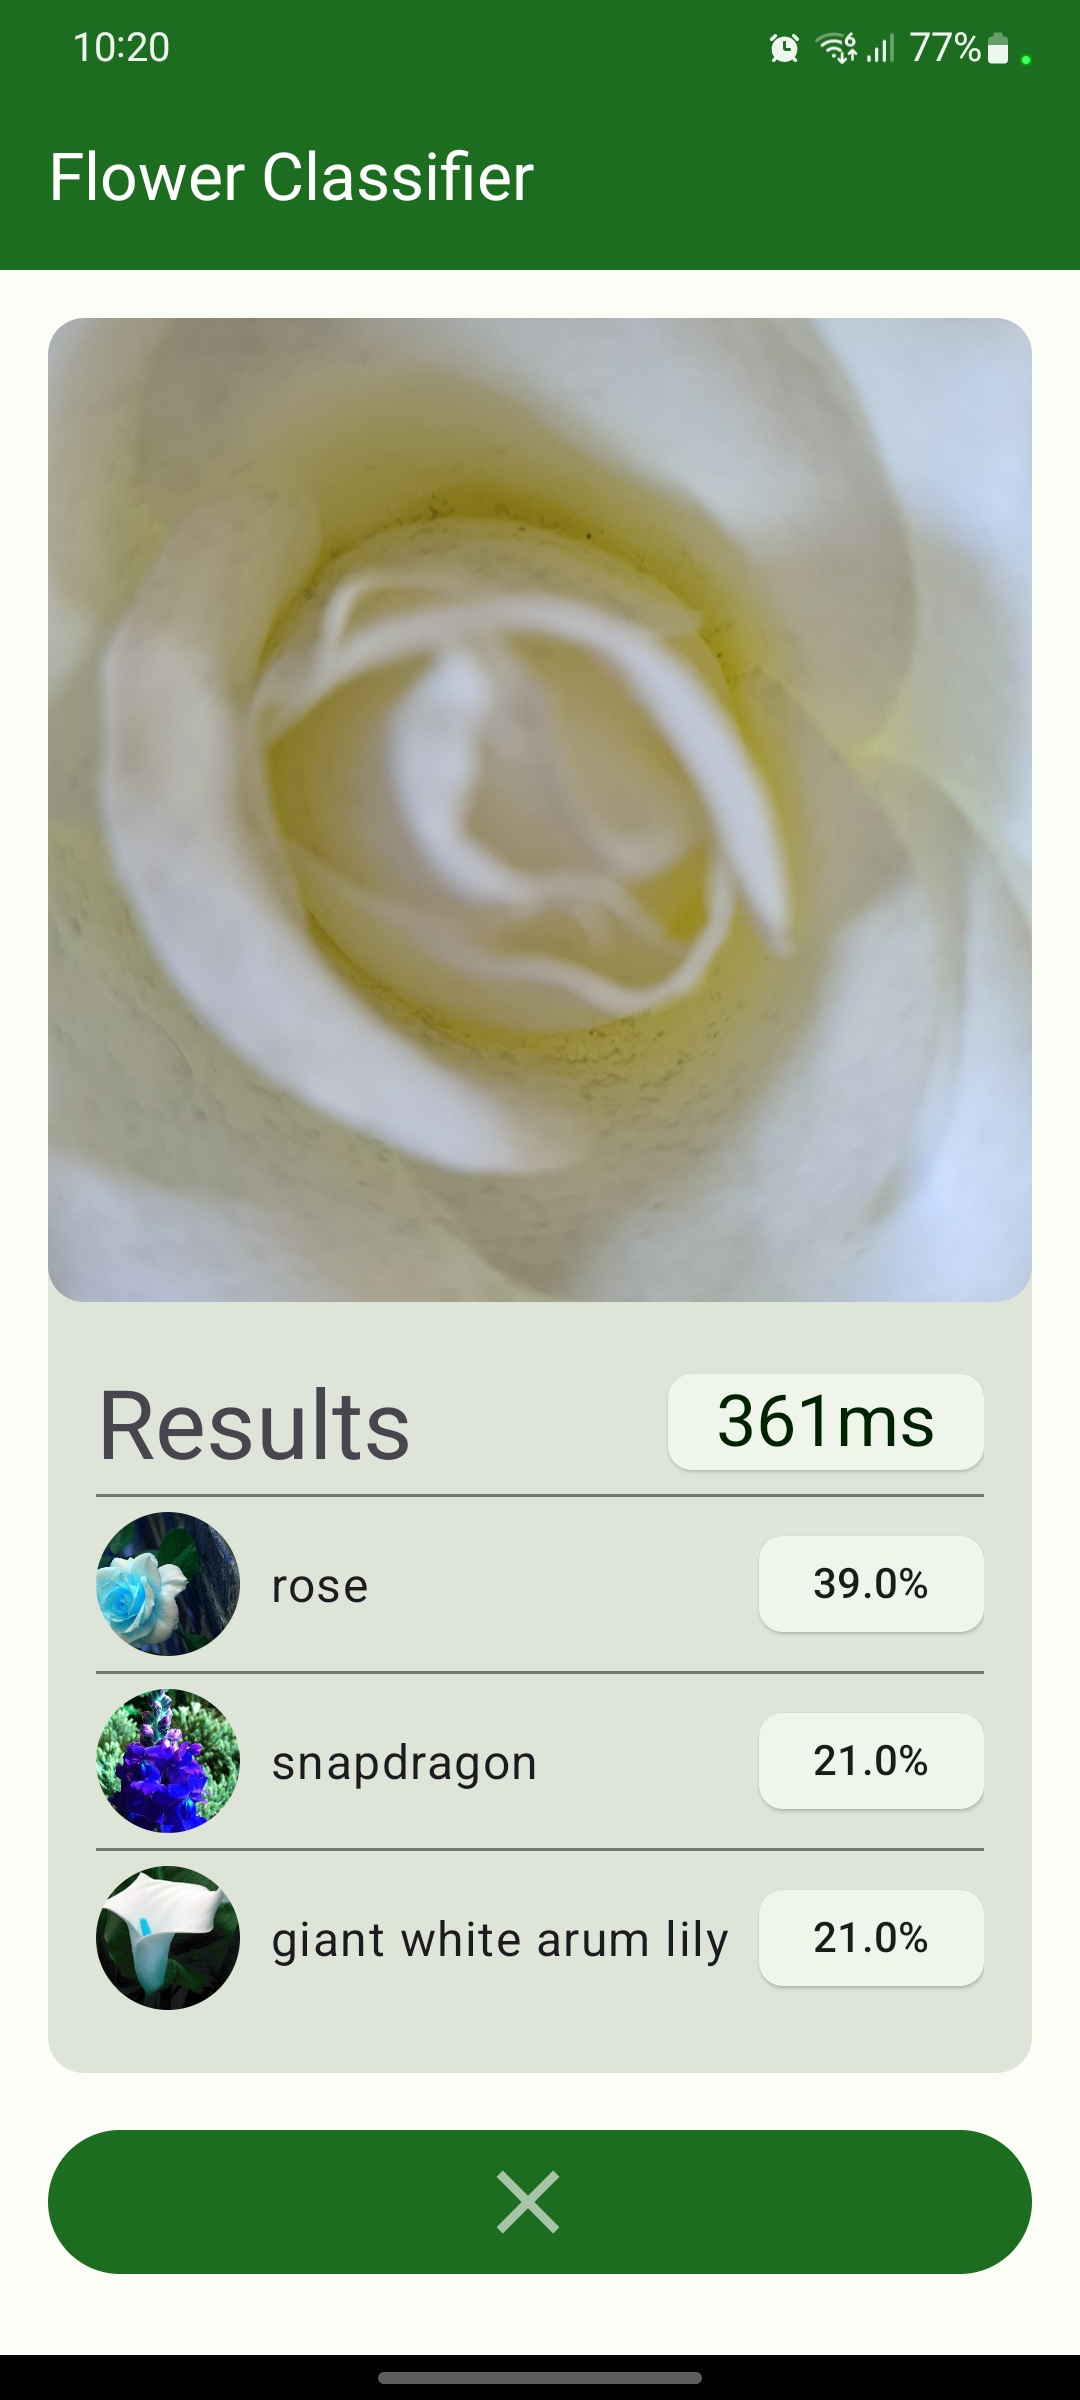
\includegraphics[width=0.3\textwidth]{rose_4cm.jpg}
    \caption{Classifying a Rose at 4cm distance using the app.}
    \label{fig:rose_4}
\end{figure}

\begin{figure}[h]\
    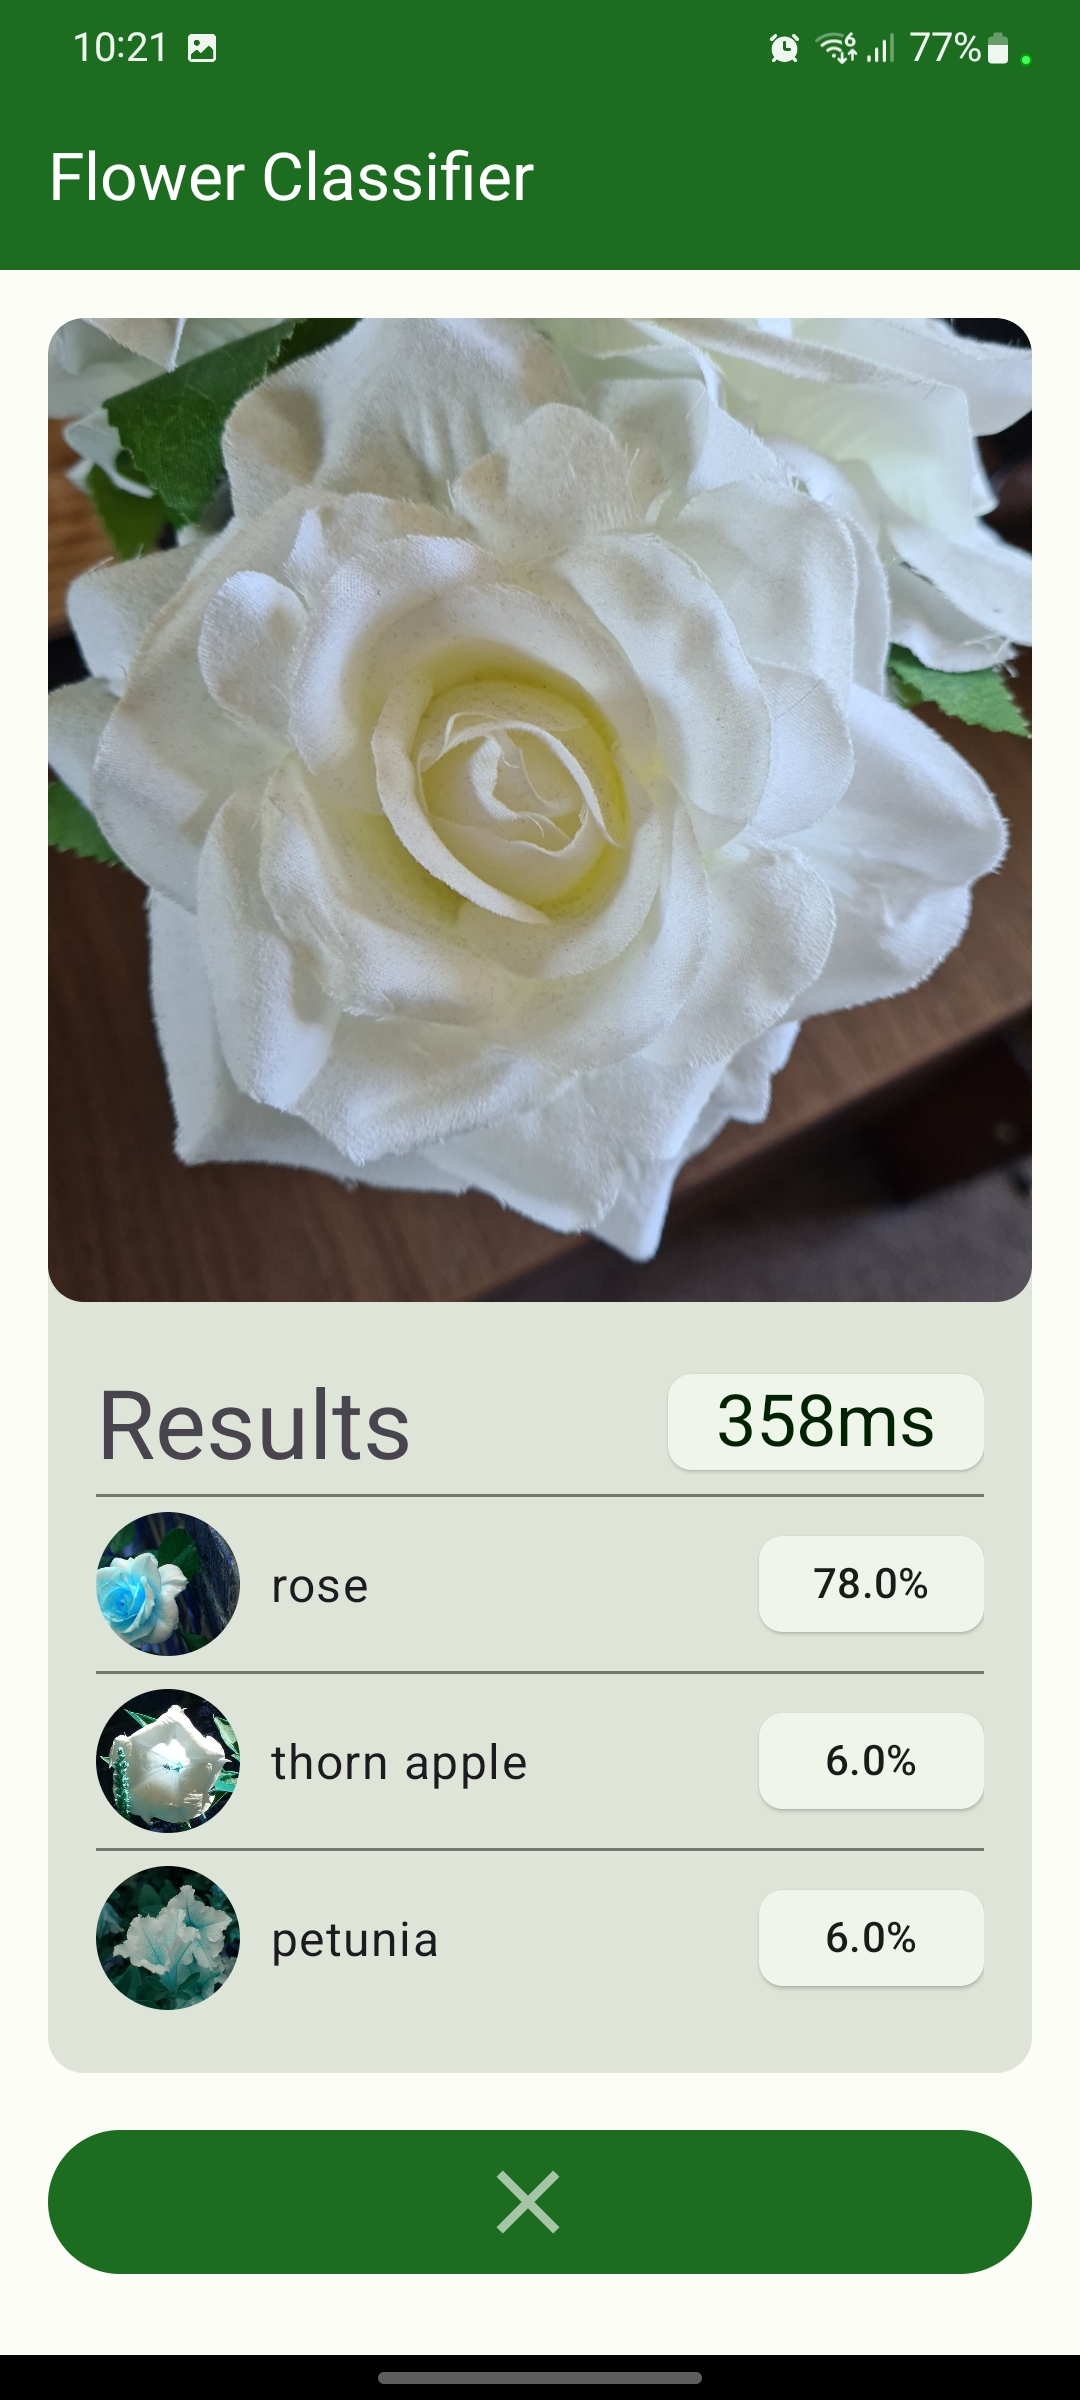
\includegraphics[width=0.3\textwidth]{rose_15cm.jpg}
    \caption{Classifying a Rose at 15cm distance using the app.}
    \label{fig:rose_15}
\end{figure}

\begin{figure}[h]\
    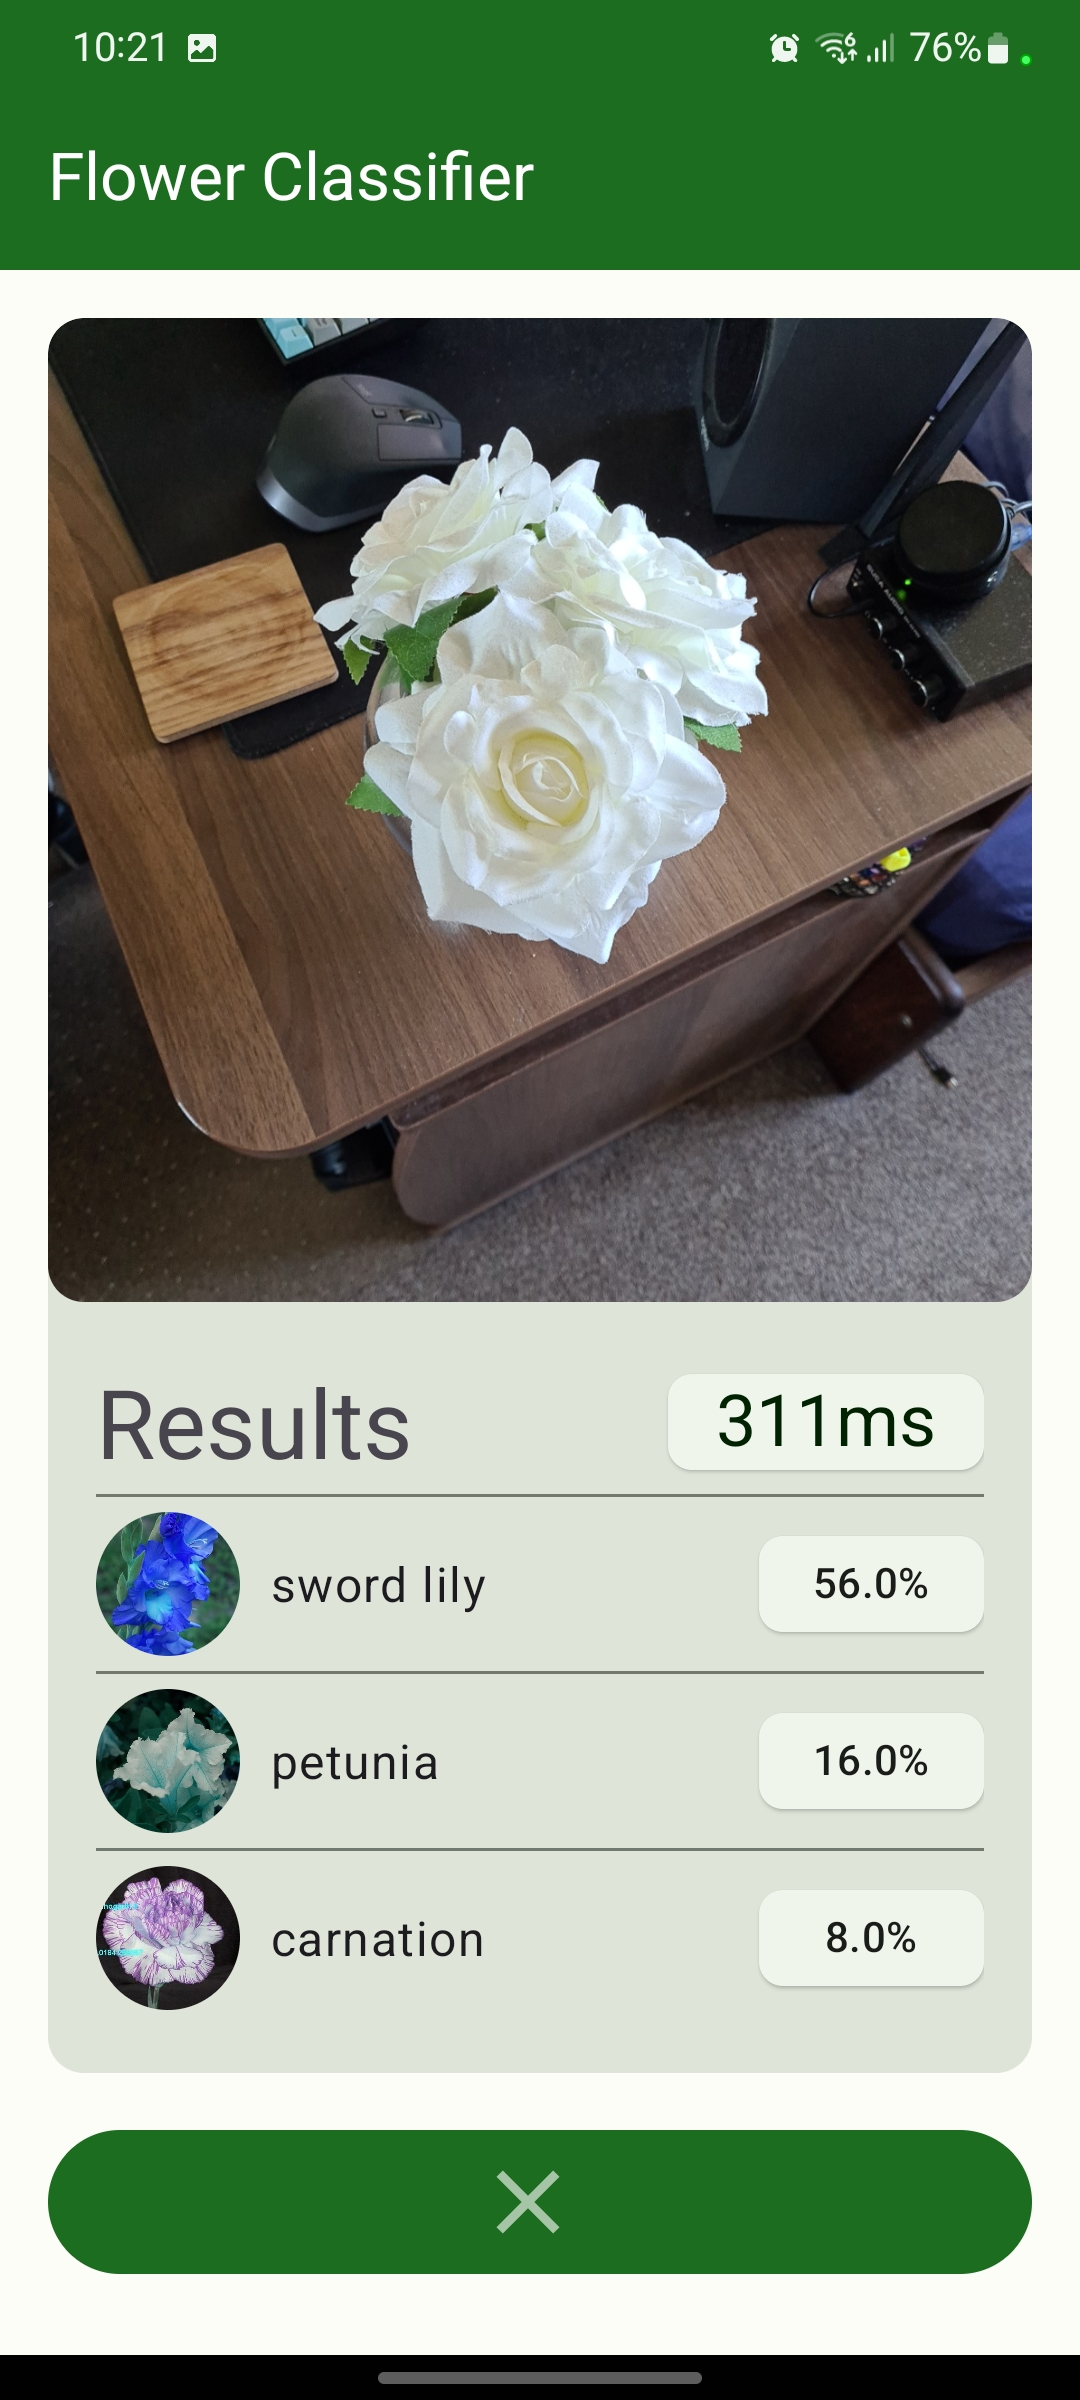
\includegraphics[width=0.3\textwidth]{rose_35cm.jpg}
    \caption{Classifying a Rose at 35cm distance using the app.}
    \label{fig:rose_35}
\end{figure}

\begin{figure}[h]\
    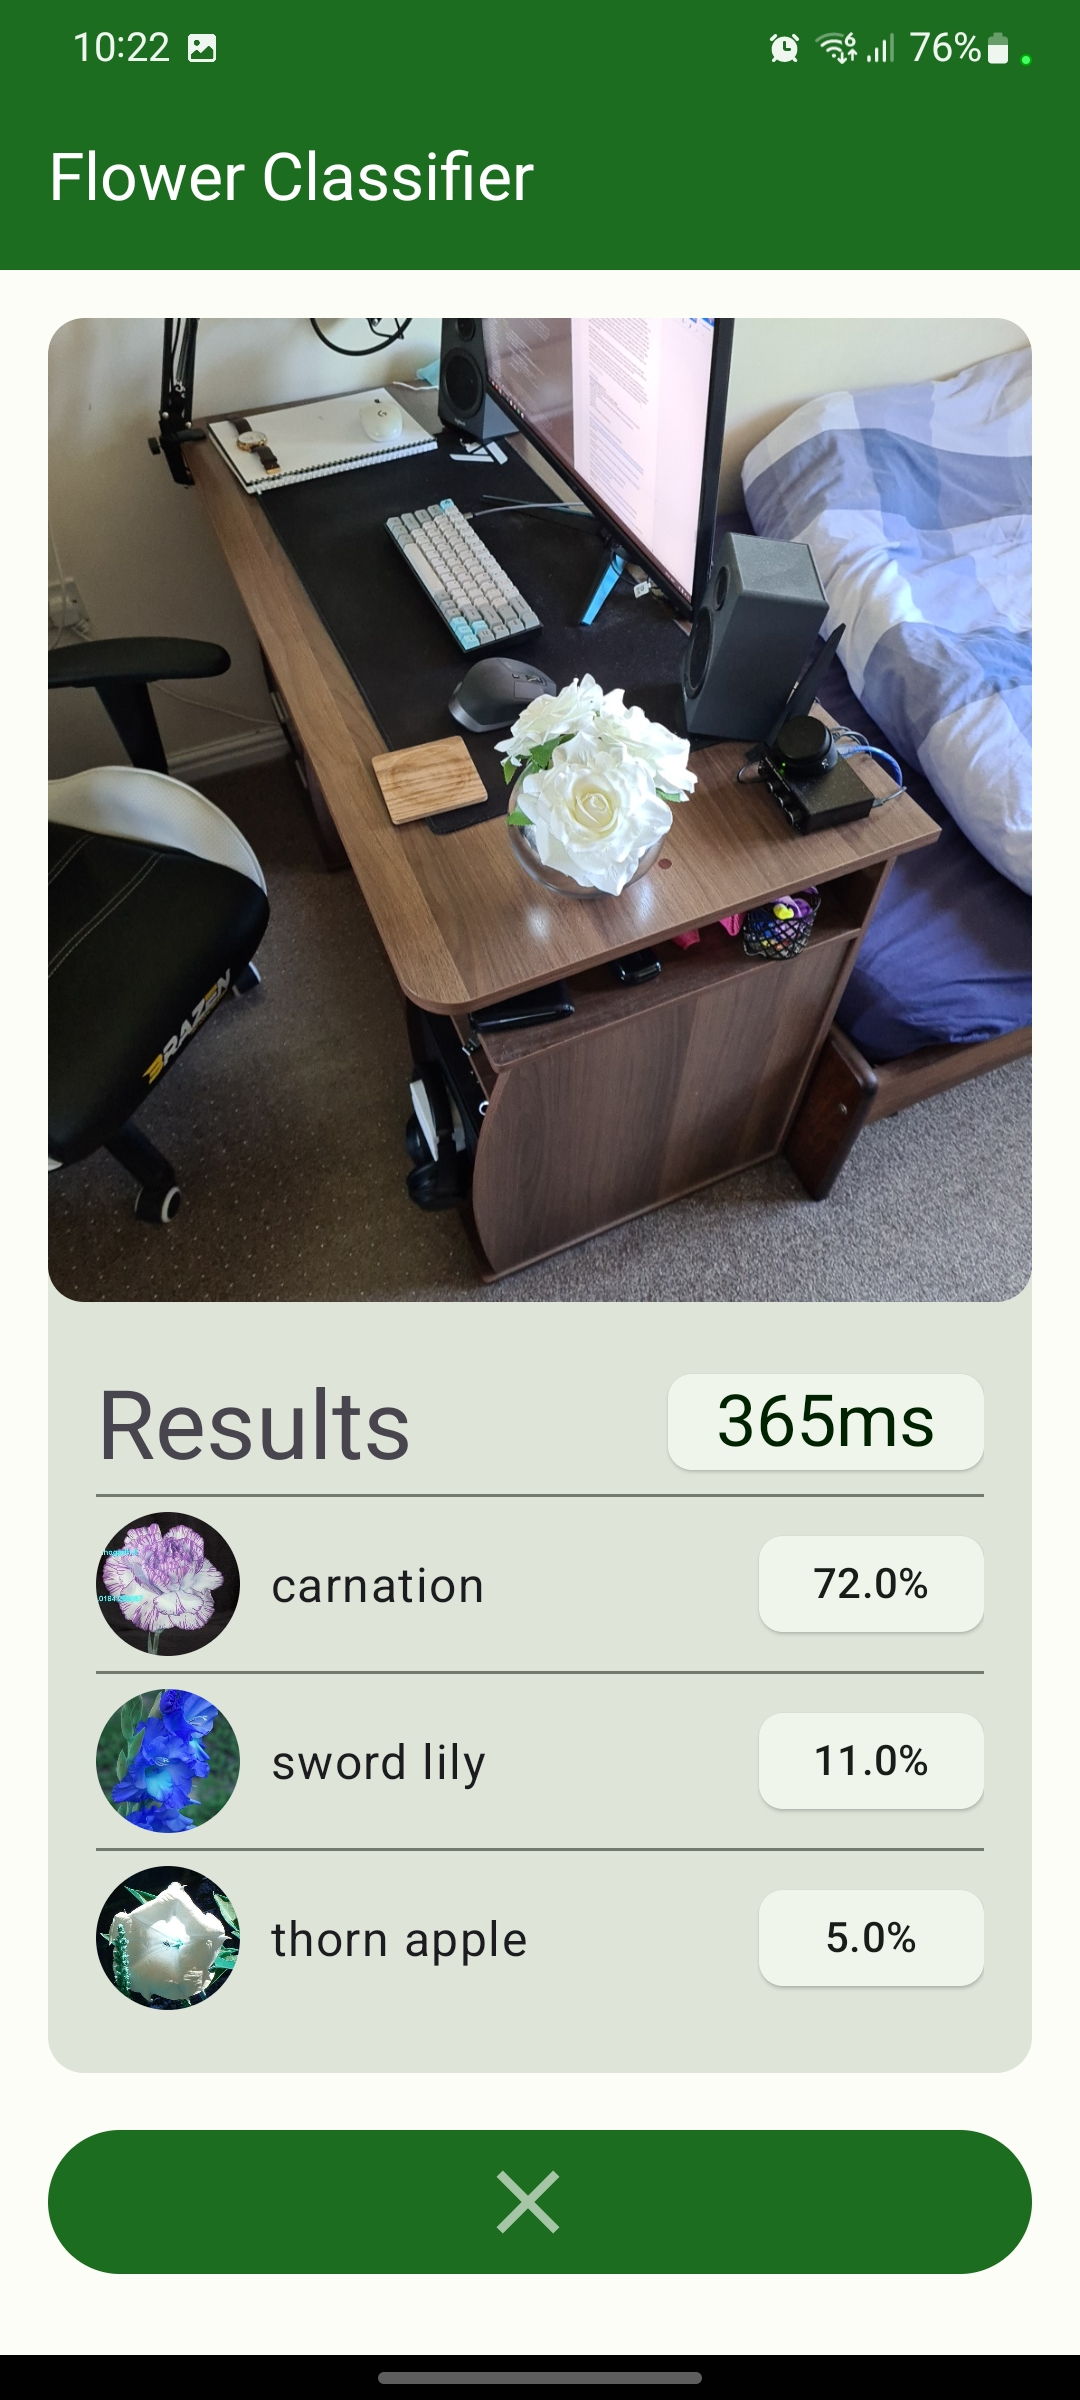
\includegraphics[width=0.3\textwidth]{rose_60cm.jpg}
    \caption{Classifying a Rose at 60cm distance using the app.}
    \label{fig:rose_60}
\end{figure}

\clearpage

\subsection{Results of angle testing}

\begin{figure}[h]\
    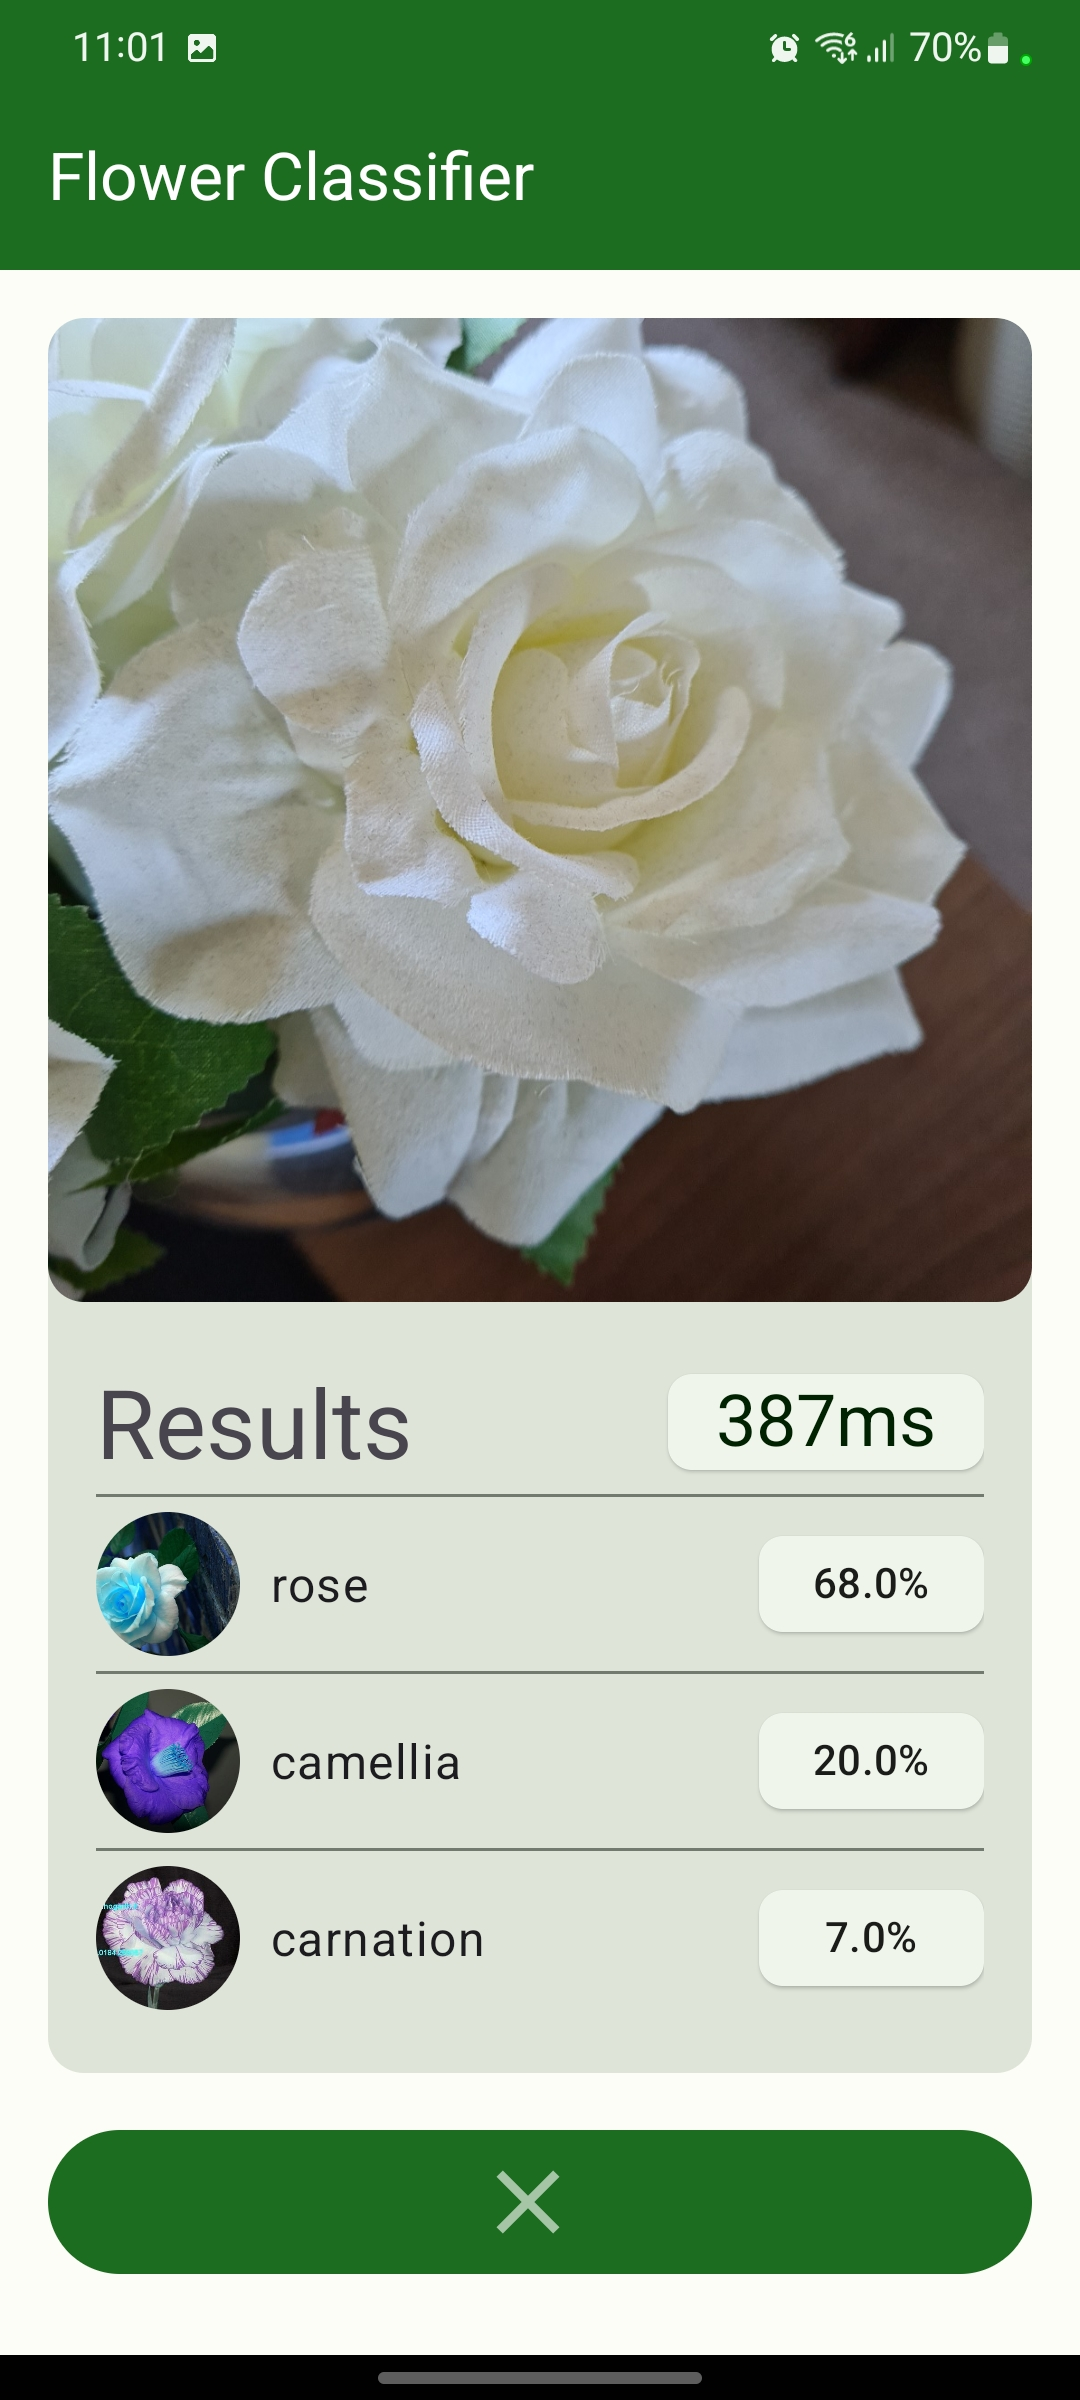
\includegraphics[width=0.3\textwidth]{rose_left.jpg}
    \caption{Classifying a Rose from the left.}
    \label{fig:rose_left}
\end{figure}

\begin{figure}[h]\
    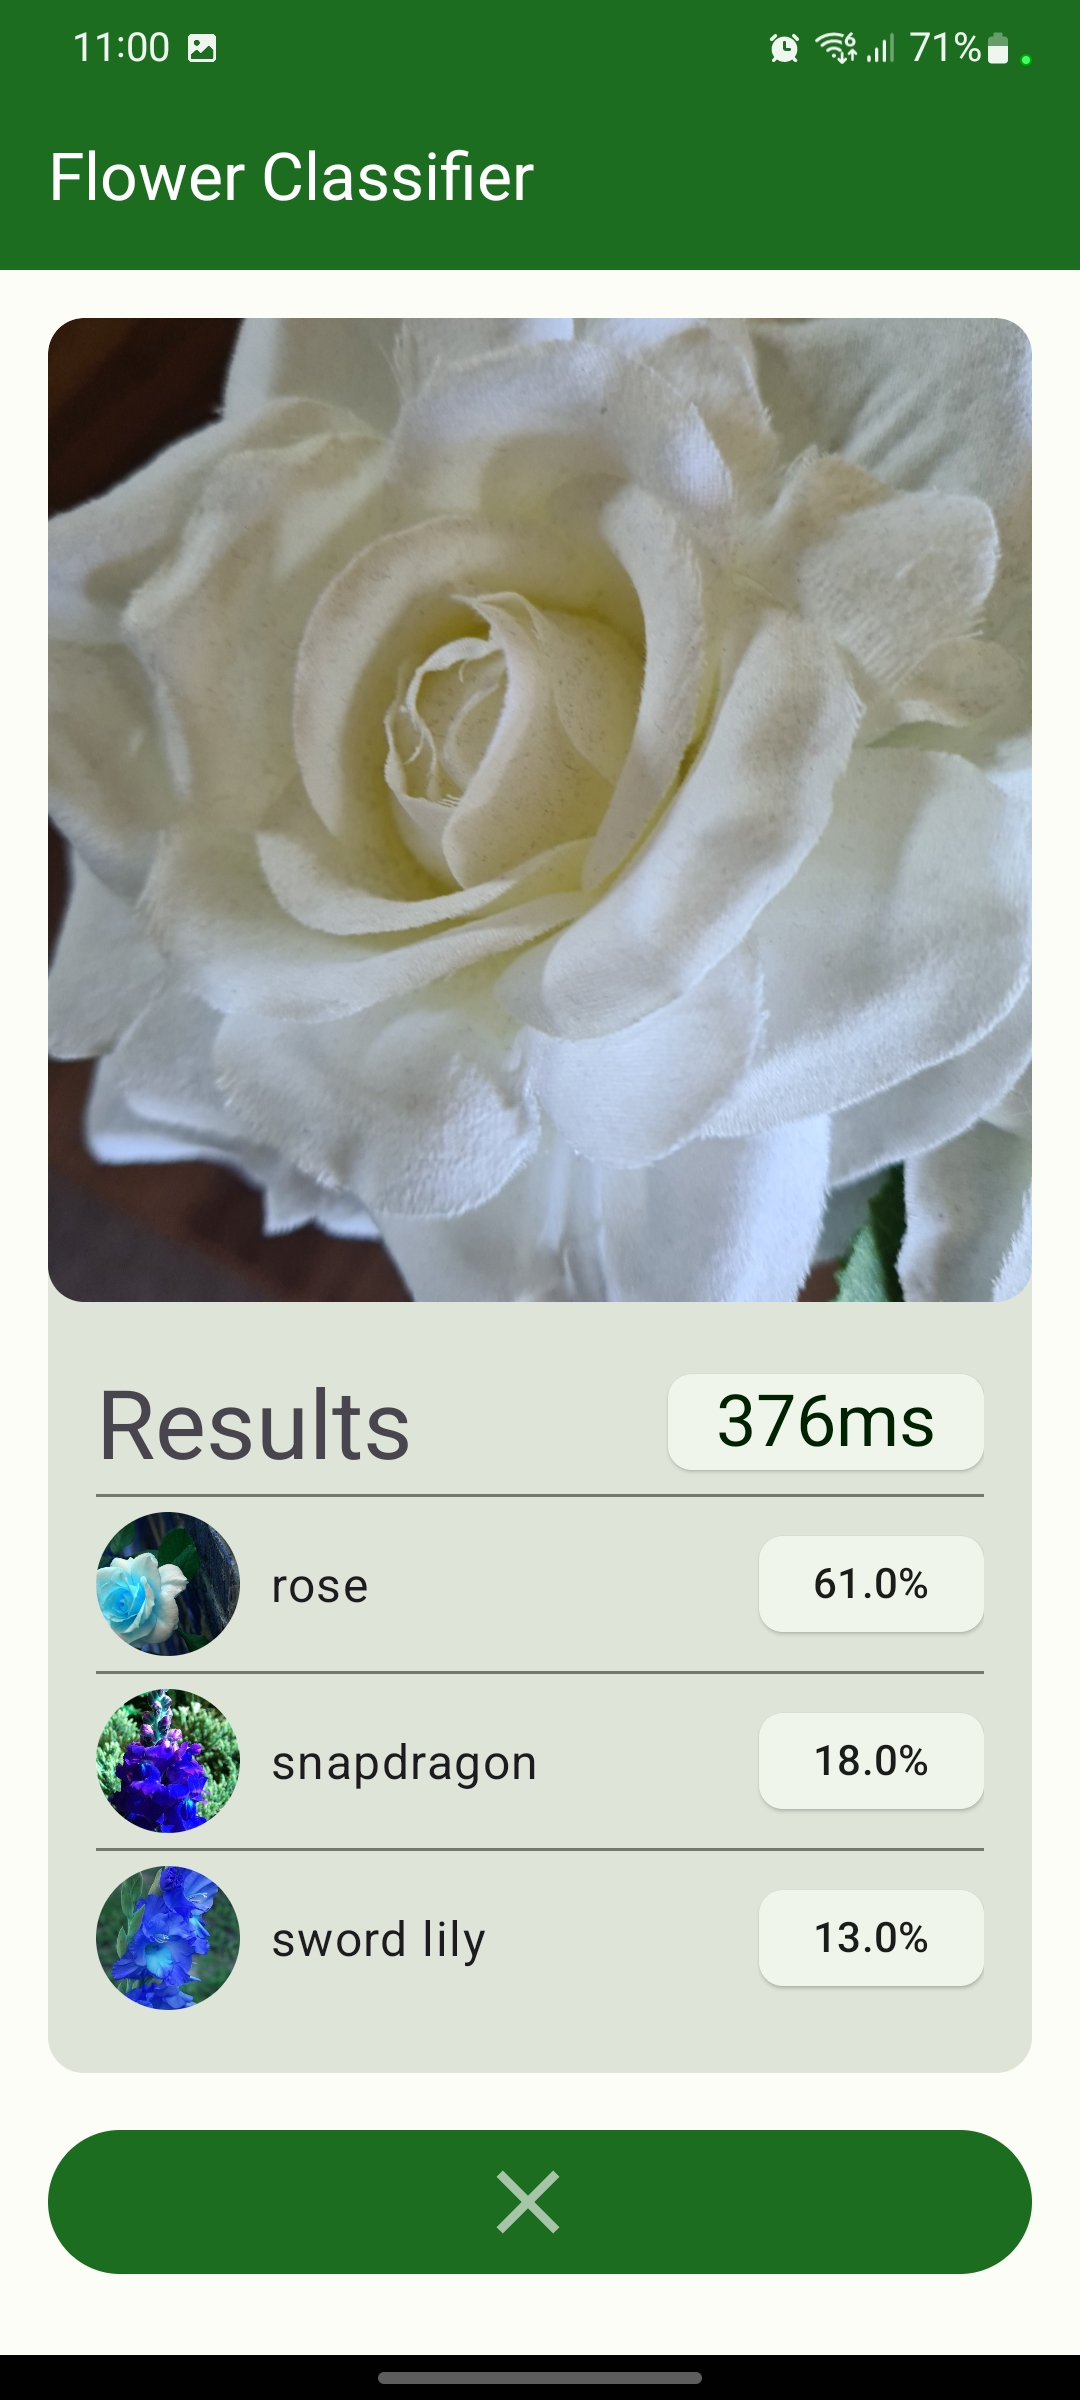
\includegraphics[width=0.3\textwidth]{rose_right.jpg}
    \caption{Classifying a Rose from the right.}
    \label{fig:rose_right}
\end{figure}

\begin{figure}[h]\
    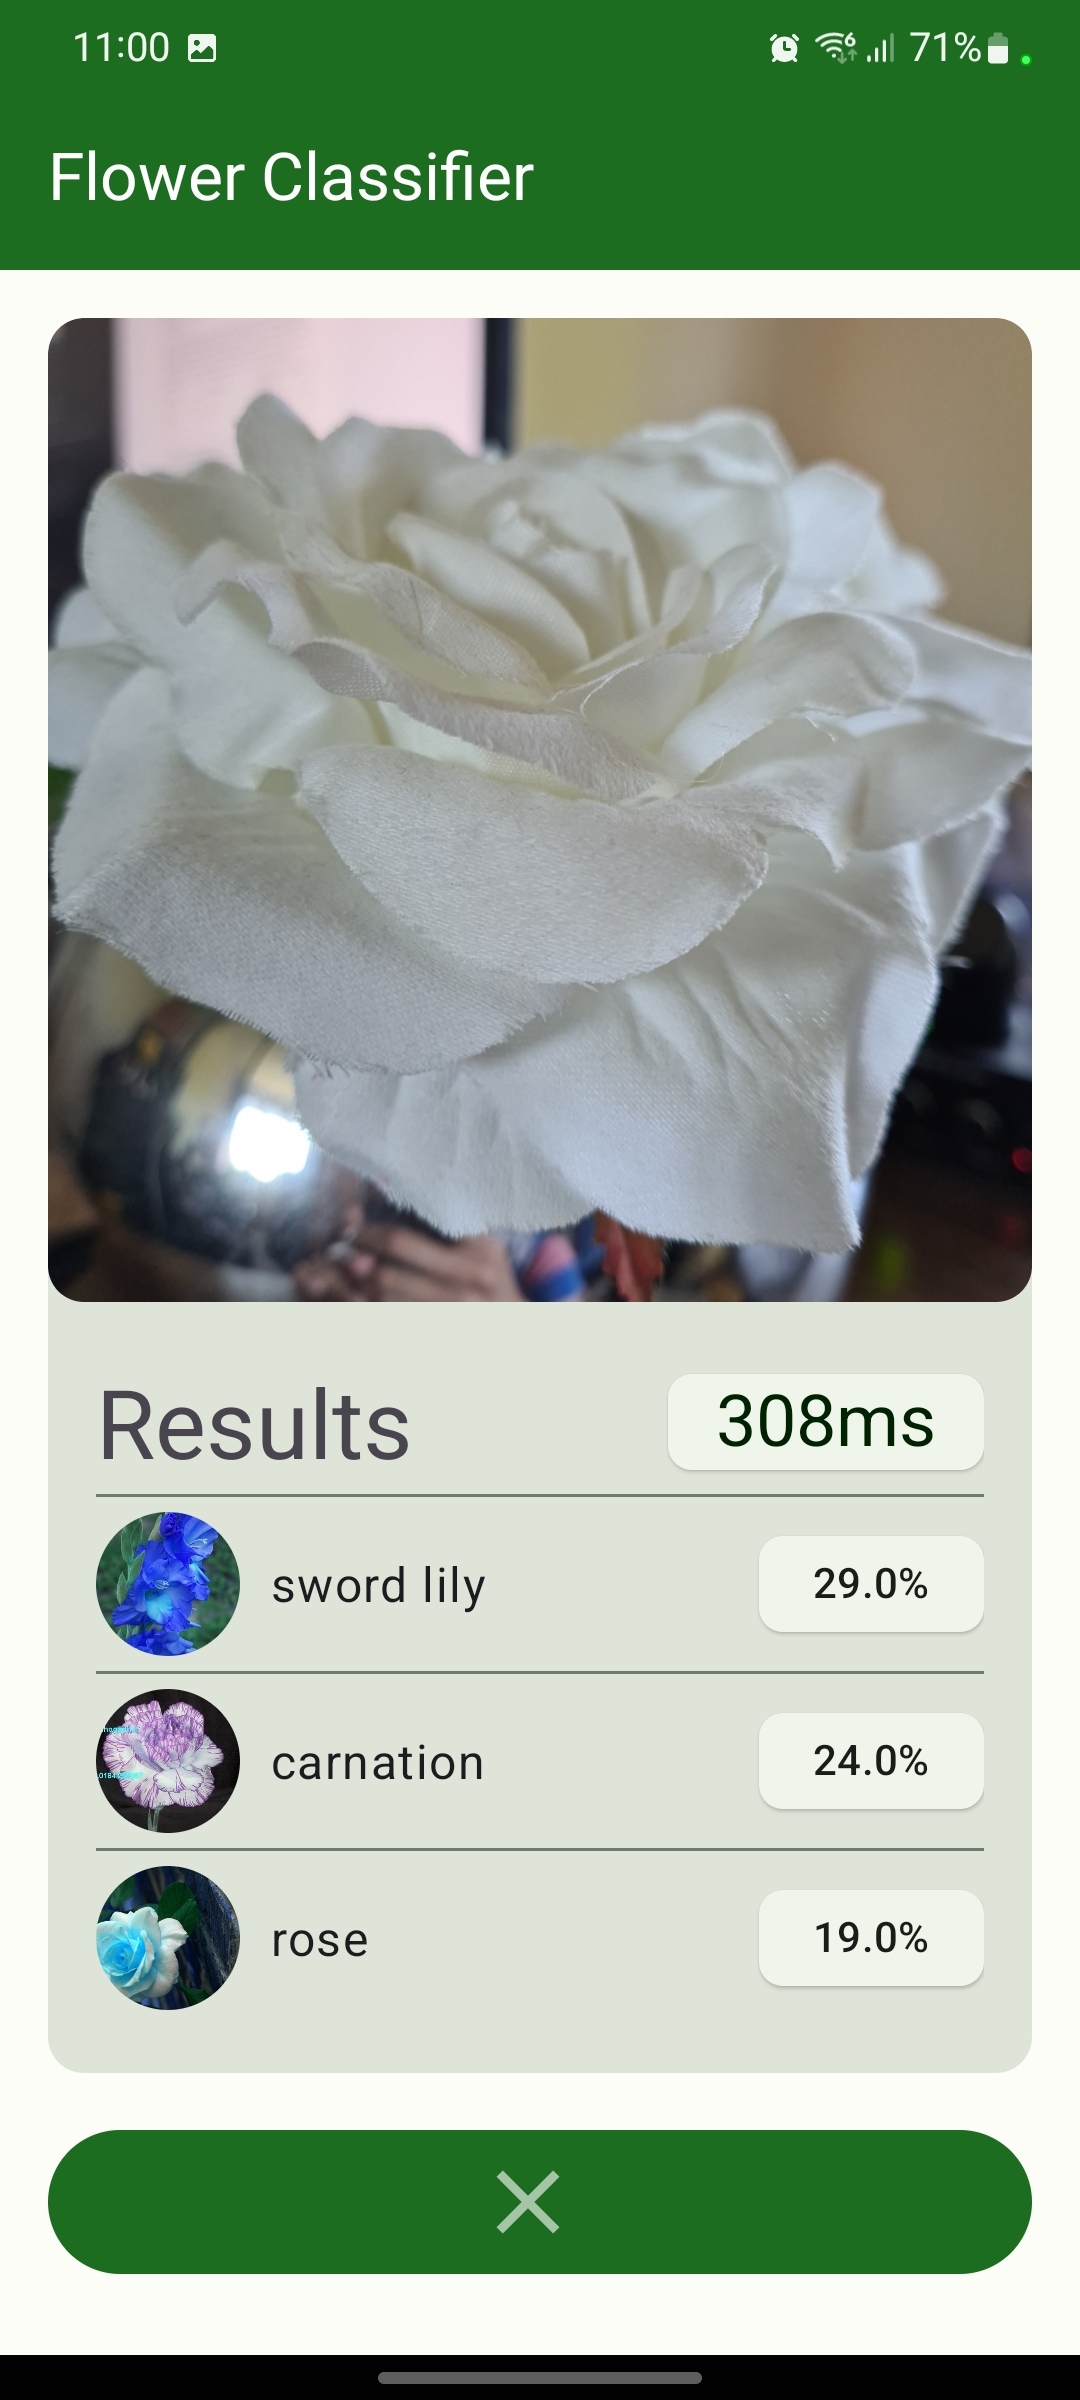
\includegraphics[width=0.3\textwidth]{rose_side.jpg}
    \caption{Classifying a Rose from the side.}
    \label{fig:rose_side}
\end{figure}

\clearpage

\subsection{Results of lighting testing}
\label{subsec:lighting}

\begin{table}[h!]
    \begin{tabular}{ |l|l|l|l| }
        \hline
        Figure & Lighting (lux) & Prediction & Prob. (\%)\\
        \hline
        \ref{fig:rose_dark} & 2.9 & Rose & 34 \\
        \hline
        \ref{fig:rose_med} & 25.4 & Rose & 68 \\
        \hline
        \ref{fig:rose_light} & 5333.6 & Thorn Apple & 45 \\
        \hline
    \end{tabular}
    \caption{Results from attempting to identify a rose at different lighting conditions.}
    \label{table:lighting}
\end{table}

\begin{figure}[h]\
    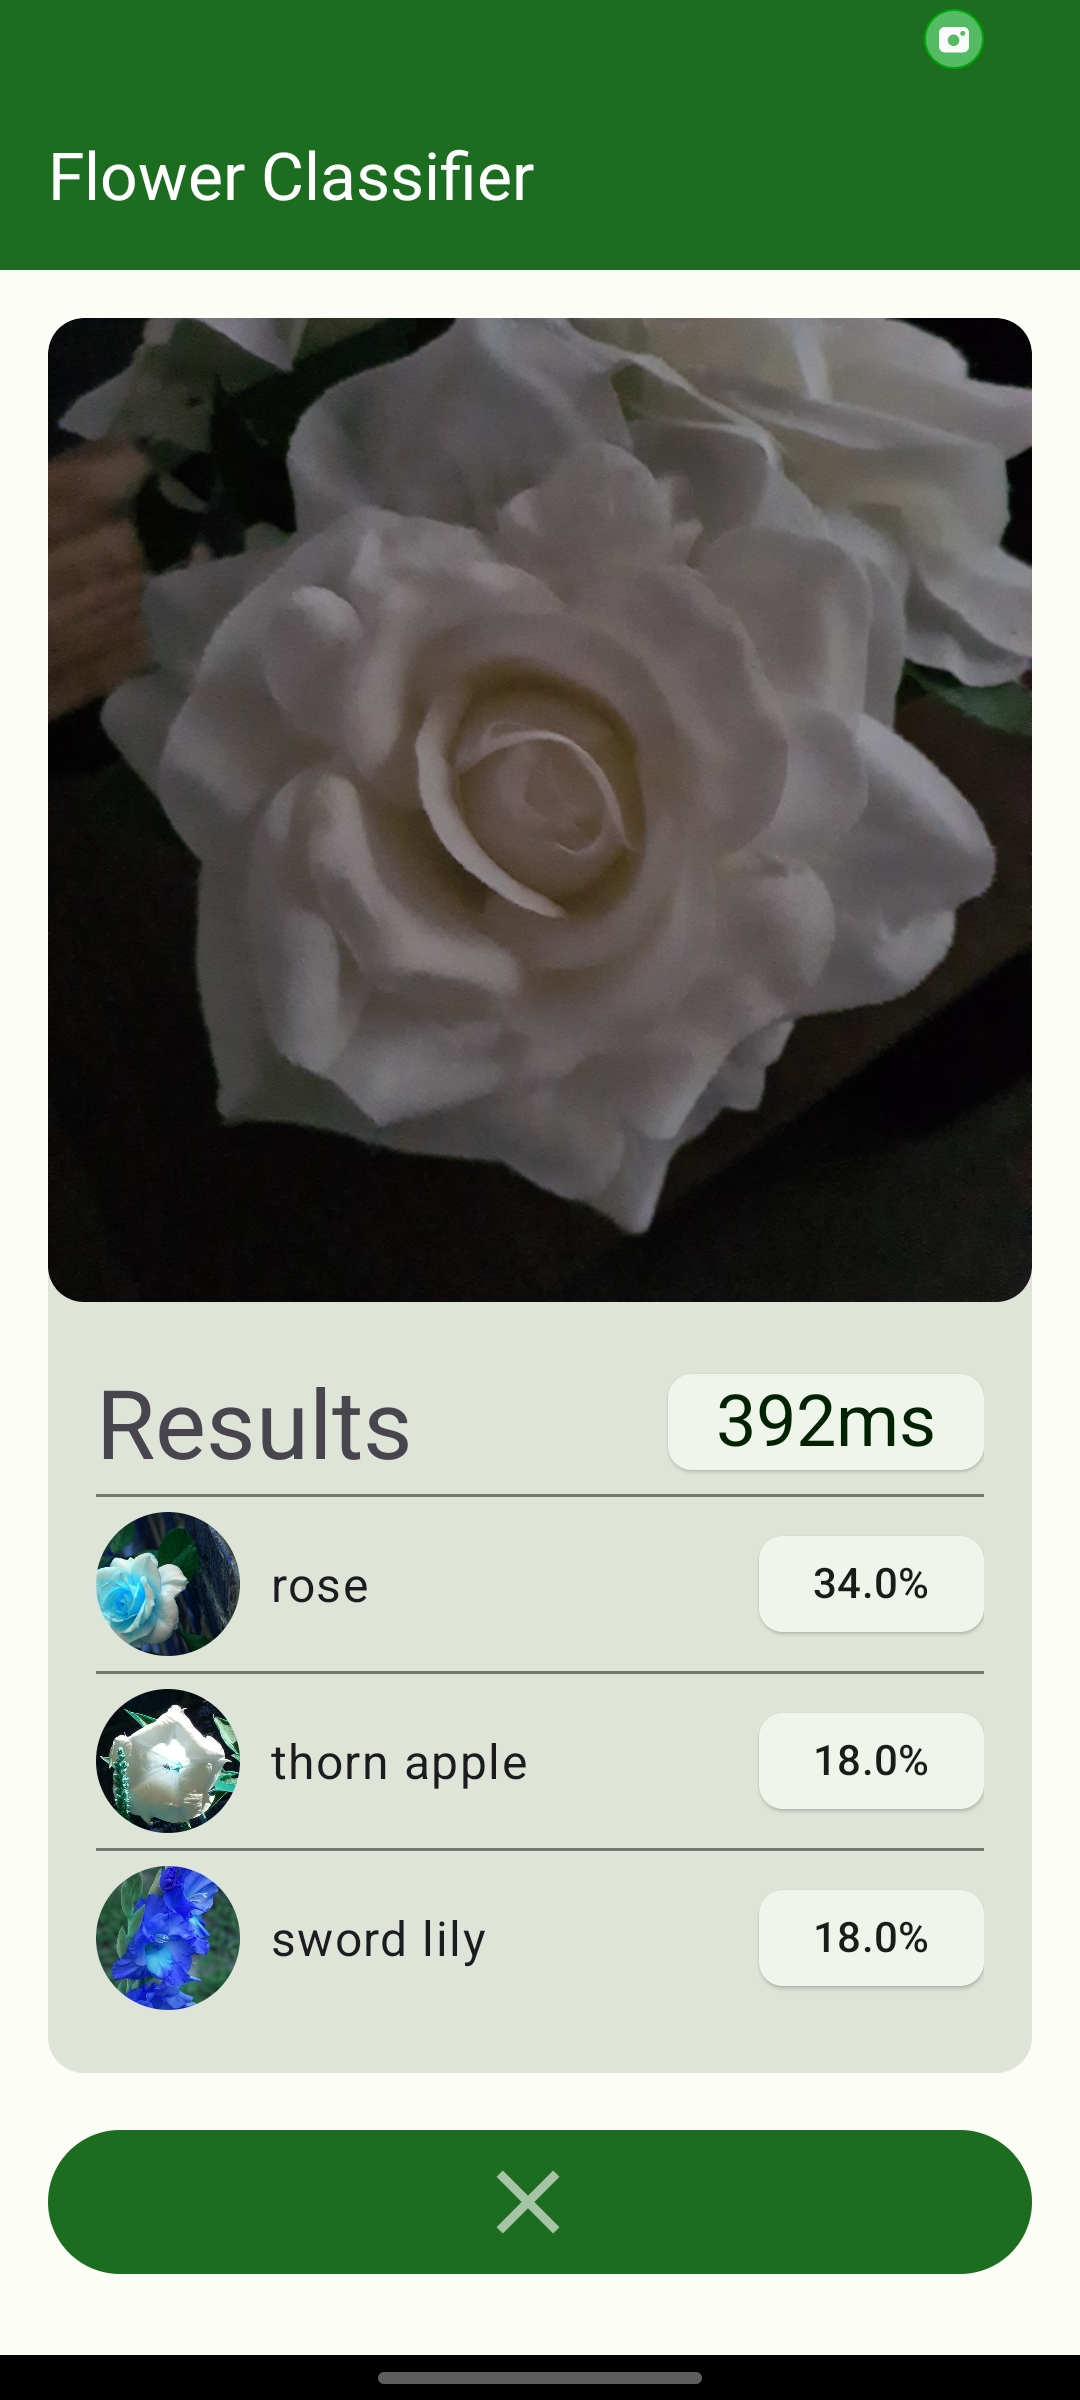
\includegraphics[width=0.3\textwidth]{rose_light_1.jpg}
    \caption{Classifying a Rose in dark conditions using the app.}
    \label{fig:rose_dark}
\end{figure}

\begin{figure}[h]\
    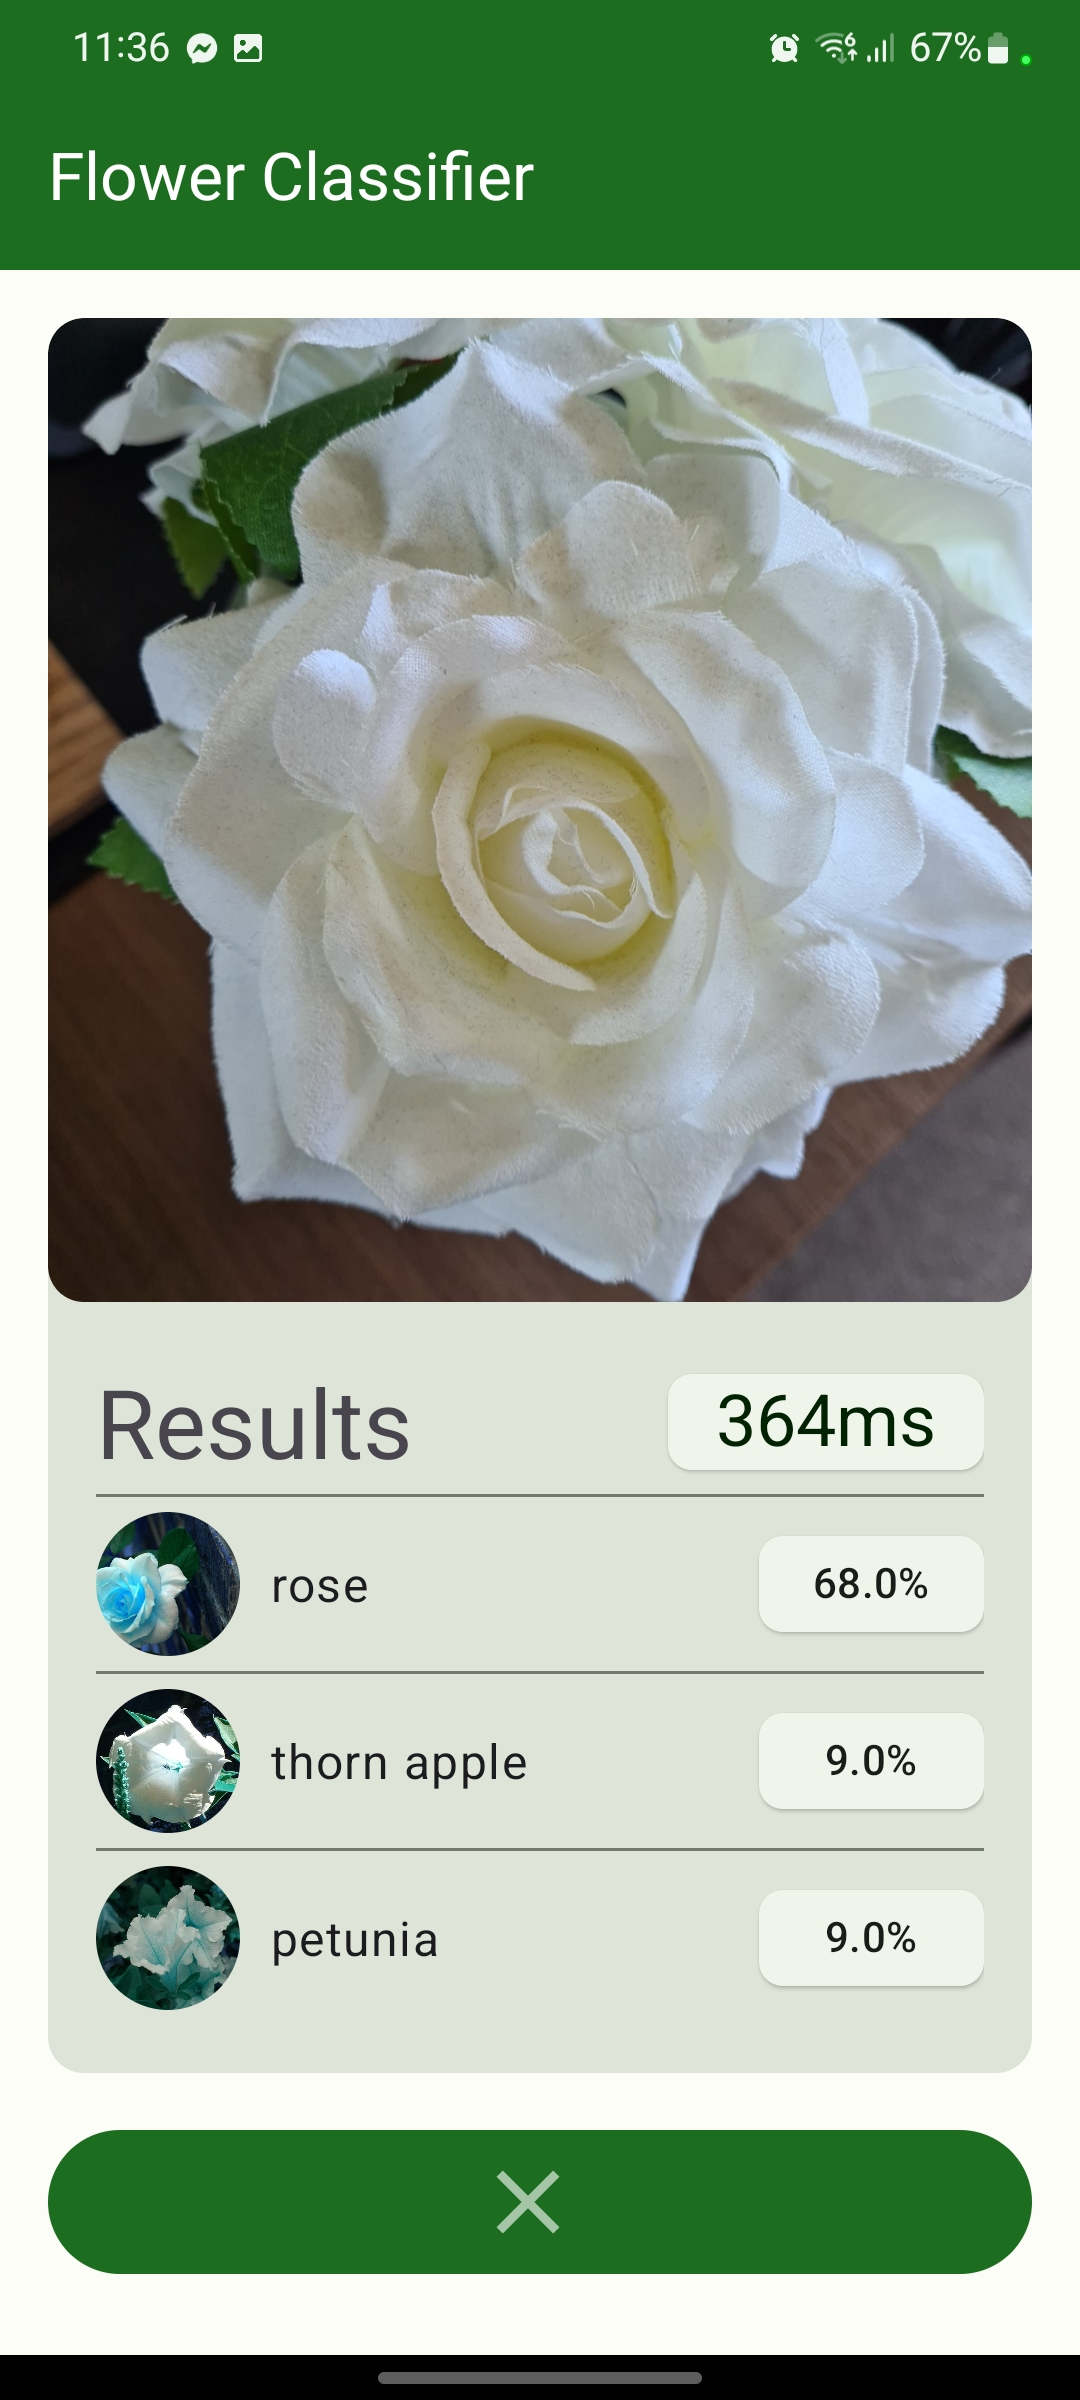
\includegraphics[width=0.3\textwidth]{rose_light_2.jpg}
    \caption{Classifying a Rose in normal conditions using the app.}
    \label{fig:rose_med}
\end{figure}

\begin{figure}[h]\
    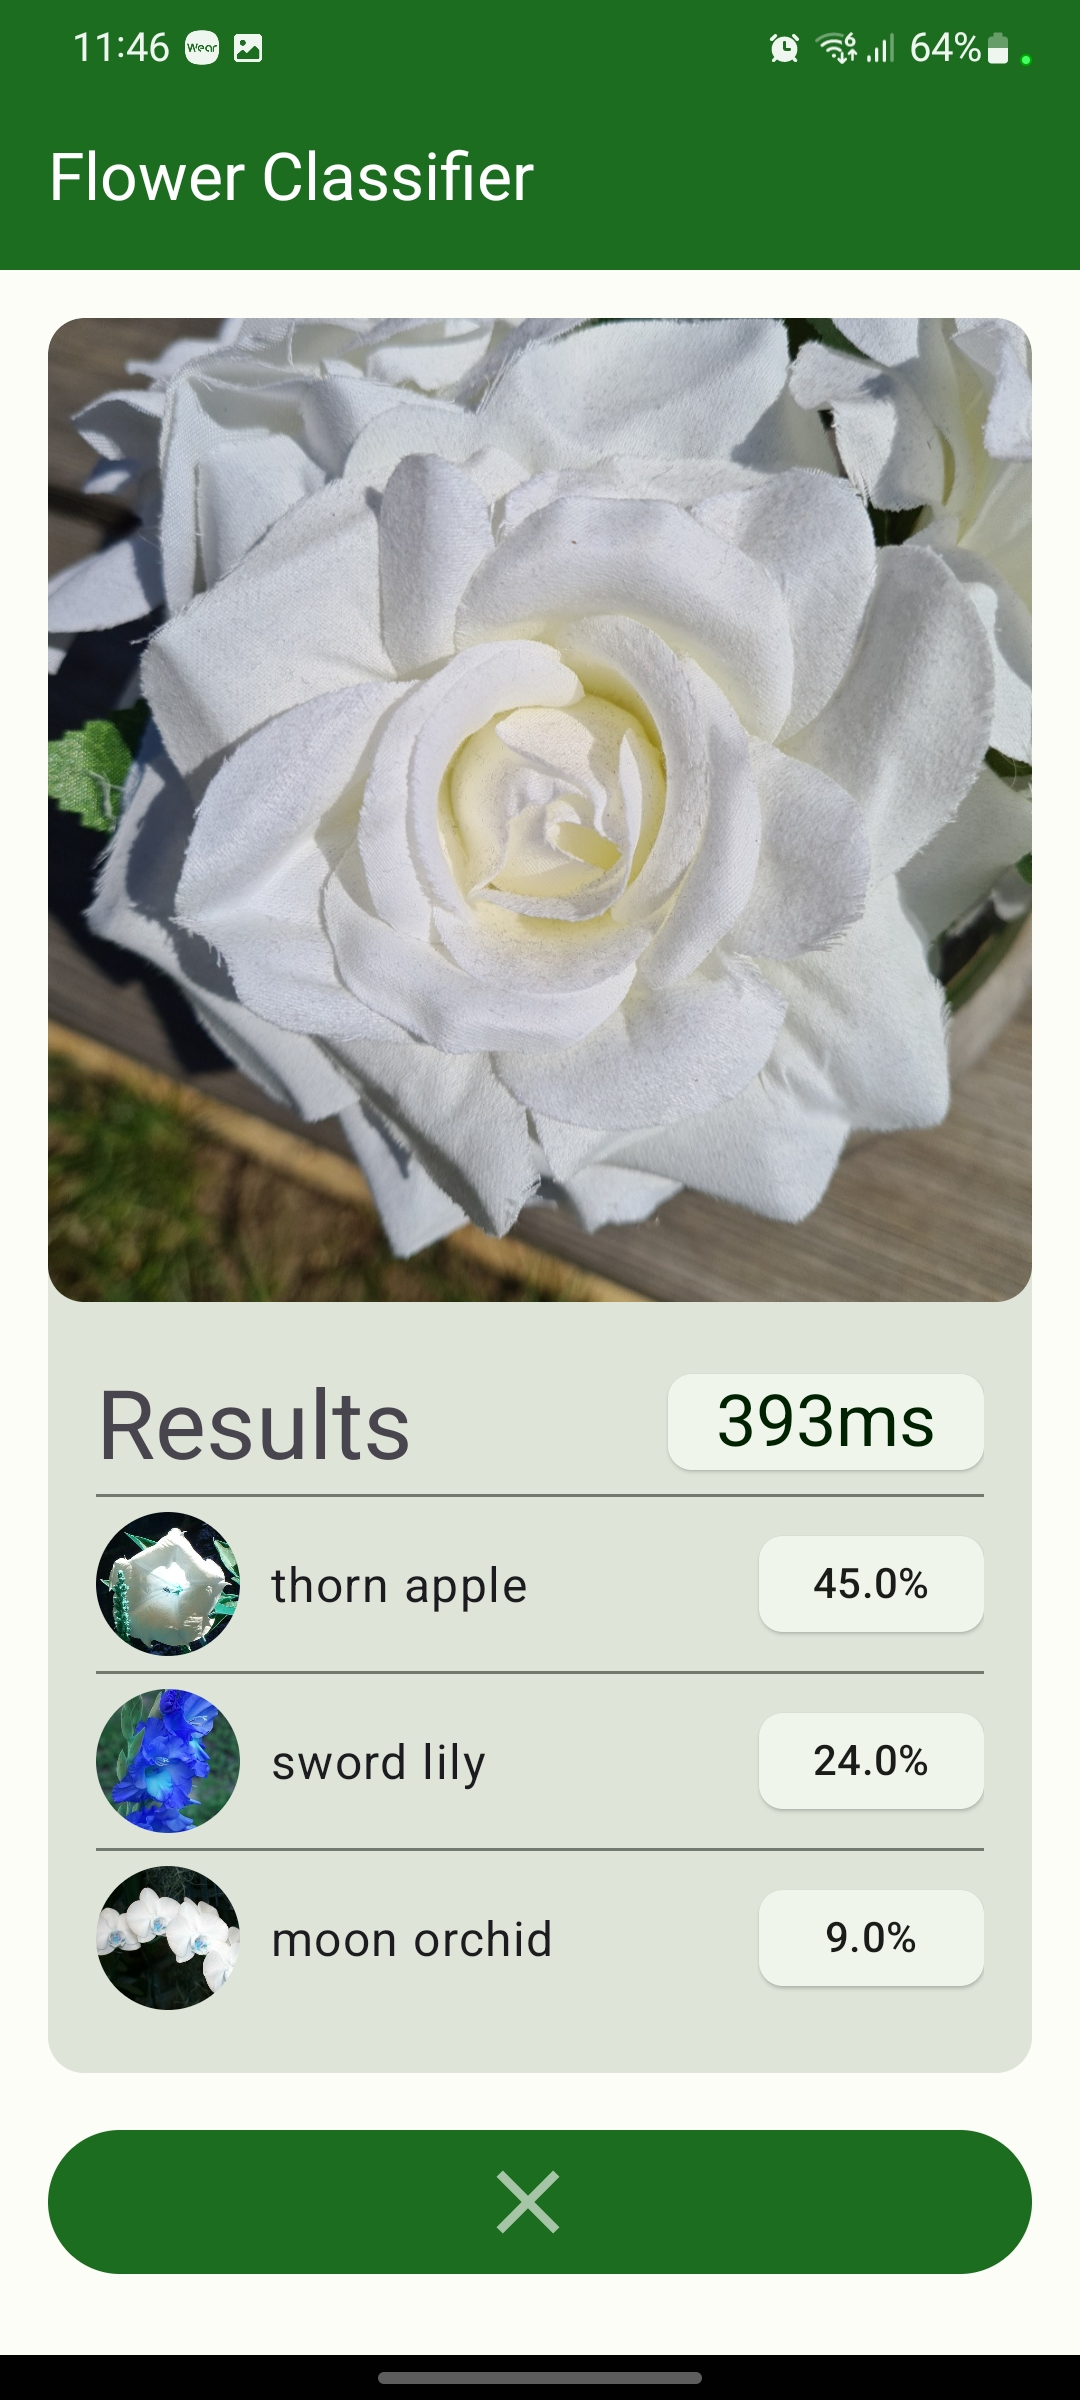
\includegraphics[width=0.3\textwidth]{rose_light_3.jpg}
    \caption{Classifying a Rose in outdoor conditions using the app.}
    \label{fig:rose_light}
\end{figure}

\clearpage

\subsection{Performance Timings}

\label{subsec:perf_timings}

\begin{figure}[h]\
    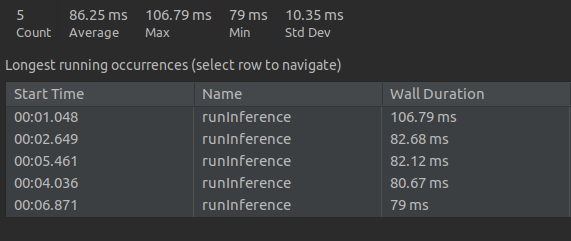
\includegraphics[width=\textwidth]{CPU1_Time.png}
    \caption{Execution timings of the CPU with 1 Thread.}
    \label{fig:cpu1}
\end{figure}


\begin{figure}[h]\
    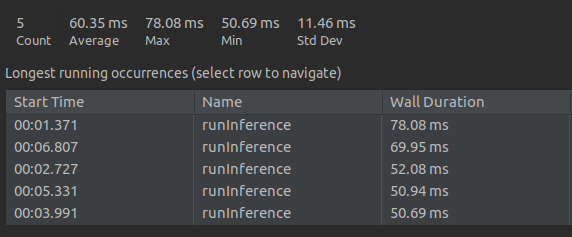
\includegraphics[width=\textwidth]{CPU2_Time.png}
    \caption{Execution timings of the CPU with 2 Threads.}
    \label{fig:cpu2}
\end{figure}

\begin{figure}[h]\
    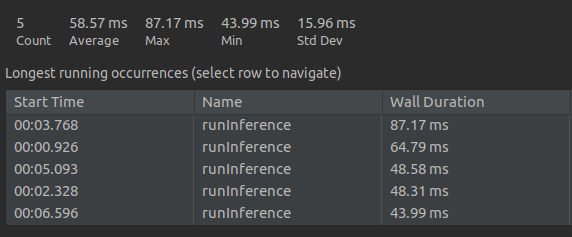
\includegraphics[width=\textwidth]{CPU4_Time.png}
    \caption{Execution timings of the CPU with 4 Threads.}
    \label{fig:cpu4}
\end{figure}

\begin{figure}[h]\
    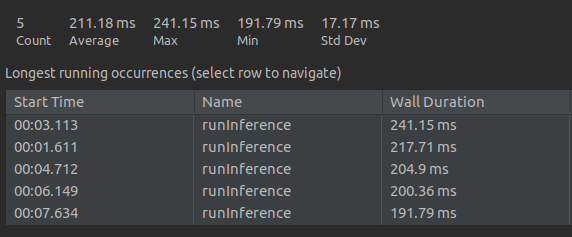
\includegraphics[width=\textwidth]{CPU8_Time.png}
    \caption{Execution timings of the CPU with 8 Threads.}
    \label{fig:cpu8}
\end{figure}

\begin{figure}[h]\
    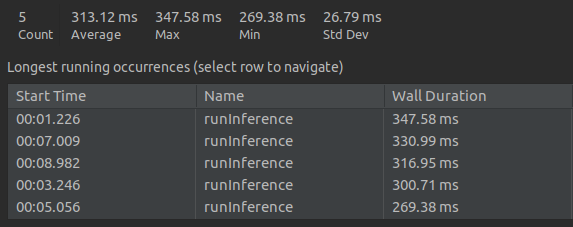
\includegraphics[width=\textwidth]{GPU_Time.png}
    \caption{Execution timings of the GPU.}
    \label{fig:gpu}
\end{figure}

\clearpage

\section{Google Image Classifier Example}

\begin{figure}[h]\
    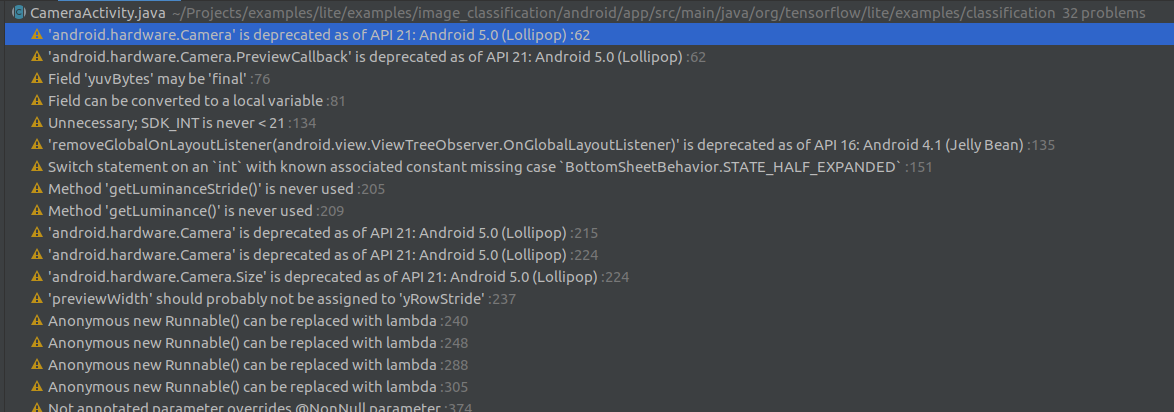
\includegraphics[width=\textwidth]{Depracated.png}
    \caption{Output from the IDE when loading the example project.}
    \label{fig:depracated}
\end{figure}

\break

\end{document}